% \iffalse
%  Local Variables:
%  mode: doctex
%  TeX-master: t
%  End:
% \fi
%
% \iffalse meta-comment
%
% Copyright (C) 2005-2010 by Ruini Xue <xueruini@gmail.com>
%
% This file may be distributed and/or modified under the
% conditions of the LaTeX Project Public License, either version 1.3a
% of this license or (at your option) any later version.
% The latest version of this license is in:
%
% http://www.latex-project.org/lppl.txt
%
% and version 1.3a or later is part of all distributions of LaTeX
% version 2004/10/01 or later.
%
% $Id$
%
% \fi
%
% \CheckSum{0}
% \CharacterTable
%  {Upper-case    \A\B\C\D\E\F\G\H\I\J\K\L\M\N\O\P\Q\R\S\T\U\V\W\X\Y\Z
%   Lower-case    \a\b\c\d\e\f\g\h\i\j\k\l\m\n\o\p\q\r\s\t\u\v\w\x\y\z
%   Digits        \0\1\2\3\4\5\6\7\8\9
%   Exclamation   \!     Double quote  \"     Hash (number) \#
%   Dollar        \$     Percent       \%     Ampersand     \&
%   Acute accent  \'     Left paren    \(     Right paren   \)
%   Asterisk      \*     Plus          \+     Comma         \,
%   Minus         \-     Point         \.     Solidus       \/
%   Colon         \:     Semicolon     \;     Less than     \<
%   Equals        \=     Greater than  \>     Question mark \?
%   Commercial at \@     Left bracket  \[     Backslash     \\
%   Right bracket \]     Circumflex    \^     Underscore    \_
%   Grave accent  \`     Left brace    \{     Vertical bar  \|
%   Right brace   \}     Tilde         \~}
%
% \iffalse
%<*driver>
\ProvidesFile{thuthesis.dtx}[2009/02/28 4.5.1 Tsinghua University Thesis Template]
\documentclass[10pt]{ltxdoc}
\usepackage{dtx-style}
\EnableCrossrefs
\CodelineIndex
\RecordChanges
%\OnlyDescription
\begin{document}
\begin{CJK*}{UTF8}{song}
  \DocInput{\jobname.dtx}
\end{CJK*}
\end{document}
%</driver>
% \fi
%
% \GetFileInfo{\jobname.dtx}
% \MakeShortVerb{\|}
%
% \def\thuthesis{\textsc{Thu}\-\textsc{Thesis}}
% \def\pkg#1{\texttt{#1}}
%
% \changes{v1.0-}{2005/07/06}{Please refer to ``Bao--Pan'' version.}
%
% \changes{v1.1}{2005/11/03}{Initial version, migrate from the old ``Bao--Pan''
% version. Make the template a class instead of package.}
%
% \changes{v1.2}{2005/11/04}{Remove \textbf{fancyref}; Remove \textbf{ucite} and implemente
% \textbf{onlinecite}; use package arial or helvet selectively.}
%
% \changes{v1.3}{2005/11/14}{replace subfigure with subfig, replace caption2
% with caption, add details about using figure in the example.}
%
% \changes{v1.4rc1}{2005/11/20}{I do not why \textbf{thu@authorizationaddon} does not work
% now for v1.3, while it's fine in v1.2. Temporarily, I remove the directive
% :(. There might be nicer solution. Other changes: add \textsf{config} option to
% subfig to be compatible with subfigure. add \textbf{courier} package for tt font.}
%
% \changes{v1.4}{2005/12/05}{Fix the problem of \textbf{chinese}, that is
% because both CJK and everysel redefined the \textbf{selectfont}. So, a not so good
% workaround is merge them up. Add \textbf{shuji} example. Add \textbf{pozhehao} command.}
%
% \changes{v2.1}{2006/02/27}{Add support to bachelor thesis.}
% \changes{v2.1}{2006/03/01}{Remove \pkg{fancyhdr} and \pkg{geometry}.}
% \changes{v2.1}{2006/03/01}{Redefine footnote marks.}
% \changes{v2.1}{2006/03/01}{Replace thubib.bst with chinesebst.bst.}
% \changes{v2.1}{2006/03/02}{Merge the modification of \pkg{ntheorem}.}
% \changes{v2.1}{2006/03/02}{Remove \pkg{footmisc} and refine the document.}
% \changes{v2.1}{2006/03/03}{Work very hard on the document.}
% \changes{v2.1}{2006/03/03}{Add |checklab| code to reduce ``unresolved labels'' warning}
% \changes{v2.2}{2006/03/26}{Adjust margins. How bad it is to simulate MS WORD!.}
% \changes{v2.2}{2006/03/26}{Add bachelor training overview details supporting.}
% \changes{v2.2}{2006/03/26}{CJK support in preamble.}
% \changes{v2.2}{2006/03/26}{Adjust hyperref to avoid boxes around links.}
% \changes{v2.3}{2006/04/07}{Fix a great bug: \cmd{PassOptionsToClass} and \cs{LoadClass}
% rather than \cs{PassOptionToPackage} and \cs{LoadPackage}.}
% \changes{v2.3}{2006/04/07}{Reorganize the codes in cover, make the pagestyle more readable.}
% \changes{v2.3}{2006/04/07}{Add gbk2uni into the document.}
% \changes{v2.3}{2006/04/07}{Support openright and openany.}
% \changes{v2.3}{2006/04/09}{Adjust hypersetup to remove color and box.}
% \changes{v2.3}{2006/04/09}{Adjust margins again.}
% \changes{v2.3}{2006/04/09}{Adjust references formats.}
% \changes{v2.3}{2006/04/09}{Redefine frontmatter and mainmatter to fit our case.}
% \changes{v2.3}{2006/04/09}{Add assumption environment.}
% \changes{v2.3}{2006/04/09}{Change the brace in the cover.}
% \changes{v2.4}{2006/04/14}{Fill more pdf info. with hypersetup.}
% \changes{v2.4}{2006/04/14}{自动隐藏密级为内部时后面的五角星。}
% \changes{v2.4}{2006/04/14}{增加``注释(Remark)''环境。}
% \changes{v2.4}{2006/04/14}{压缩 item 之间的距离。}
% \changes{v2.4}{2006/04/14}{thubib.bst 文献标题取消自动小写。}
% \changes{v2.4}{2006/04/14}{中文参考文献取消 In: Proceedings。}
% \changes{v2.4}{2006/04/14}{英文文参考文献调整 In: editor, Proceedings。}
% \changes{v2.4}{2006/04/14}{参考文献为学位论文时,加方括号,作者后面为实心点。}
% \changes{v2.4}{2006/04/14}{中文参考文献作者超过三个加等。}
% \changes{v2.4}{2006/04/14}{中文参考文献需要在 bib 中指定 |lang="chinese"|。}
% \changes{v2.4}{2006/04/14}{学位论文不在需要 type 字段。}
% \changes{v2.4}{2006/04/14}{为摘要等条目增加书签。}
% \changes{v2.4}{2006/04/14}{章节的编号用黑体,也就是自动打开 arialtitle 选项。}
% \changes{v2.4.1}{2006/04/17}{2.4 忘了把关键词的 tabular 改成 thu@tabular。}
% \changes{v2.4.1}{2006/04/17}{参考文献最后一个作者前是逗号而不是 and。}
% \changes{v2.4.2}{2006/04/18}{去掉参考文献第二个作者后面烦人的逗号。}
% \changes{v2.5}{2006/05/19}{对本科论文进行大幅度的重写,因为教务处修改了格式要求。}
% \changes{v2.5}{2006/05/19}{重新整理代码,使其布局更易读。}
% \changes{v2.5.1}{2006/05/24}{根据教务处的新要求调整附录部分。}
% \changes{v2.5.1}{2006/05/25}{参考文献中杂志文章如果没有卷号,那么页码直接跟在
% 年份后面,并用句点分割。在 thubib.bst 中增加 output.year 函数。}
% \changes{v2.6.1}{2006/06/16}{取消 thubib.bst 中 inbook 类 volume 后的页码。}
% \changes{v4.5}{2008/01/04}{彻底转向 UTF-8,并支持 xelatex。}
%
% \DoNotIndex{\begin,\end,\begingroup,\endgroup}
% \DoNotIndex{\ifx,\ifdim,\ifnum,\ifcase,\else,\or,\fi}
% \DoNotIndex{\let,\def,\xdef,\newcommand,\renewcommand}
% \DoNotIndex{\expandafter,\csname,\endcsname,\relax,\protect}
% \DoNotIndex{\Huge,\huge,\LARGE,\Large,\large,\normalsize}
% \DoNotIndex{\small,\footnotesize,\scriptsize,\tiny}
% \DoNotIndex{\normalfont,\bfseries,\slshape,\interlinepenalty}
% \DoNotIndex{\hfil,\par,\hskip,\vskip,\vspace,\quad}
% \DoNotIndex{\centering,\raggedright}
% \DoNotIndex{\c@secnumdepth,\@startsection,\@setfontsize}
% \DoNotIndex{\ ,\@plus,\@minus,\p@,\z@,\@m,\@M,\@ne,\m@ne}
% \DoNotIndex{\@@par,\DeclareOperation,\RequirePackage,\LoadClass}
% \DoNotIndex{\AtBeginDocument,\AtEndDocument}
%
% \IndexPrologue{\section*{索引}%
%    \addcontentsline{toc}{section}{索~~~~引}}
% \GlossaryPrologue{\section*{修改记录}%
%    \addcontentsline{toc}{section}{修改记录}}
%
% \renewcommand{\abstractname}{摘~~要}
% \renewcommand{\contentsname}{目~~录}
%
%
% \title{\thuthesis:清华大学学位论文模板\thanks{Tsinghua University \LaTeX{} Thesis Template.}}
% \author{{\fs 薛瑞尼\thanks{LittleLeo@newsmth}}\\[5pt]{\fs 清华大学计算机系高性能所}\\[5pt] \texttt{xueruini@gmail.com}}
% \date{v\fileversion\ (\filedate)}
% \maketitle\thispagestyle{empty}
%
%
% \begin{abstract}\noindent
%   此宏包旨在建立一个简单易用的清华大学学位论文模板,包括本科综合论文训练、硕士
%   论文、博士论文以及博士哲学论文。现在已经支持本科、硕士和博士论文格式,对其它
%   格式的支持会陆续加入。
% \end{abstract}
%
% \vskip2cm
% \def\abstractname{免责声明}
% \begin{abstract}
% \noindent
% \begin{enumerate}
% \item 本模板的发布遵守 \LaTeX{} Project Public License,使用前请认真阅读协议内容。
% \item 本模板为作者根据清华大学教务处颁发的《综合论文训练写作指南》和清华大学研
%   究生院颁发的《研究生学位论文写作指南》编写而成,旨在供清华大学毕业生撰写学位
%   论文使用。
% \item 清华大学教务处和研究生院只提供毕业论文写作指南,不提供官方模板,也不会授
%   权第三方模板为官方模板,所以此模板仅为写作指南的参考实现,不保证格式审查老师
%   不提意见。任何由于使用本模板而引起的论文格式审查问题均与本模板作者无关。
% \item 任何个人或组织以本模板为基础进行修改、扩展而生成的新的专用模板,请严格遵
%   守 \LaTeX{} Project Public License 协议。由于违犯协议而引起的任何纠纷争端均与
%   本模板作者无关。
% \end{enumerate}
% \end{abstract}
%
%
% \clearpage
% \begin{multicols}{2}[
%   \section*{\contentsname}
%   \setlength{\columnseprule}{.4pt}
%   \setlength{\columnsep}{18pt}]
%   \tableofcontents
% \end{multicols}
%
% \clearpage
% \pagenumbering{arabic}
% \pagestyle{headings}
% \section{模板介绍}
% \thuthesis\ (\textbf{T}sing\textbf{hu}a \textbf{Thesis}) 是为了帮助清华大学毕业
% 生撰写毕业论文而编写的 \LaTeX{} 论文模板。
%
% 本文档将尽量完整的介绍模板的使用方法,如有不清楚之处可以参考示例文档或者给邮件
% 列表(见后)写信,欢迎感兴趣的同学出力完善此使用手册。由于个人水平有限,虽然现
% 在的这个版本基本上满足了学校的要求,但难免还存在不足之处,欢迎大家积极反馈。
%
% {\color{blue}\fs 模板的作用在于减轻论文写作过程中格式调整的时间,其前提就是遵
%   守模板的用法,否则即使使用了 \thuthesis{} 也难以保证输出的论文符合学校规范。}
%
%
% \section{安装}
% \label{sec:installation}
%
% \subsection{下载}
% \thuthesis{} 主页:\url{http://thuthesis.sourceforge.net}。同时本模板也提交至
% \href{http://www.ctan.org/macros/latex/contrib/thuthesis}{CTAN}。除此之外,不
% 再维护任何镜像。
%
% \thuthesis{} 的开发版本同样可以在 sourceforge 上获得:
% \begin{shell}
% $ svn co https://svn.sourceforge.net/svnroot/thuthesis/trunk/thuthesis
% \end{shell}
%
% \subsection{模板的组成部分}
% 下表列出了 \thuthesis{} 的主要文件及其功能介绍:
%
% \begin{center}
%   \begin{longtable}{l|p{10cm}}
% \hline
% {\hei 文件(夹)} & {\hei 功能描述}\\\hline\hline
% \endfirsthead
% \hline
% {\hei 文件(夹)} & {\hei 功能描述}\\\hline\hline
% \endhead
% \endfoot
% \endlastfoot
% thuthesis.ins & 模板驱动文件 \\
% thuthesis.dtx & 模板文档代码的混合文件\\
% thuthesis.cls & 模板类文件\\
% thuthesis.cfg & 模板配置文件\\
% thubib.bst & 参考文献样式文件\\\hline
% main.tex & 示例文档主文件\\
% shuji.tex & 书脊示例文档\\
% ref/ & 示例文档参考文献目录\\
% data/ & 示例文档章节具体内容\\
% figures/ & 示例文档图片路径\\
% thutils.sty & 为示例文档加载其它宏包\\\hline
% Makefile & self-explanation \\
% msmake.cmd & Windows 批处理工具\\\hline
% Readme & self-explanation\\
% \textbf{thuthesis.pdf} & 用户手册(本文档)\\\hline
%   \end{longtable}
% \end{center}
%
% 需要说明几点:1) thuthesis.cls 和 thuthesis.cfg 可以
% 由 thuthesis.ins 和thuthesis.dtx 生成,但为了降低新手用户的使用难度,故将 cls
% 和 cfg 也一起发布。2) 学习一个新东西最好的办法就是读它的文
% 档:\emph{thuthesis.pdf}.
%
%
% \subsection{准备工作}
% \label{sec:prepare}
% 本模板用到以下宏包:
%
% \begin{center}
% \begin{minipage}{1.0\linewidth}\centering
% \begin{tabular}{*{6}{l}}\hline
%   ifxetex & xunicode & xltxtra & CJK\footnote{版本要求:$\geq$ v4.8.1} & xeCJK\footnote{\href{http://bbs.ctex.org/viewthread.php?tid=40232&extra=page%3D1}{xeCJK 下载页}} & \pkg{CJKpunct} \\
%   array & booktabs & longtable  &  amsmath & amssymb & ntheorem \\
%   indentfirst & paralist & txfonts & natbib & hyperref & hypernat \\
%   graphicx & \pkg{subfig}\footnote{版本要求:$\geq$2005/06/28 ver: 1.3} &
%   \pkg{caption}\footnote{版本要求:$\geq$2006/03/21 v3.0j} &
%   \pkg{thubib.bst} & &\\\hline
% \end{tabular}
% \end{minipage}
% \end{center}
%
% 这些包在常见的 \TeX{} 系统中都有,如果没有请到 \url{www.ctan.org} 下载。推
% 荐 \TeX live 2008。
%
%
% \subsection{开始安装}
% \label{sec:install}
%
% \subsubsection{生成模板}
% \label{sec:generate-cls}
% {\hei 说明:默认的发行包中已经包含了所有文件,可以直接使用。如果对如何由 dtx 生
%   成模板文件以及模板文档不感兴趣,请跳过本小节。}
%
% 模板解压缩后生成文件夹 thuthesis-VERSION\footnote{VERSION 为版本号。},其中包括:
% 模板源文件(thuthesis.ins 和 thuthesis.dtx),参考文献样式 thubib.bst,示例文档
% (main.tex,shuji.tex,thutils.sty\footnote{我把可能用到但不一定用到的包以及一
%   些命令定义都放在这里面,以免 thuthesis.cls 过分臃
%   肿。},data/ 和 figures/ 和 ref/)。在使用之前需要先生成模板文件和配置文件
% (具体命令细节请参考 |Readme| 和 |Makefile|):
%
% \begin{shell}
% $ cd thuthesis-VERSION
% # 生成 thuthesis.cls 和 thuthesis.cfg
% $ latex thuthesis.ins
%
% # 下面的命令用来生成用户手册,可以不执行
% $ latex thuthesis.dtx
% $ makeindex -s gind.ist -o thuthesis.ind thuthesis.idx
% $ makeindex -s gglo.ist -o thuthesis.gls thuthesis.glo
% $ latex thuthesis.dtx
% $ latex thuthesis.dtx  % 生成说明文档 thuthesis.dvi
% \end{shell}
%
%
% \subsubsection{dvi$\rightarrow$ps$\rightarrow$pdf}
% \label{sec:dvipspdf}
% 很多用户对 \LaTeX{} 命令执行的次数不太清楚,一个基本的原则是多次运行 \LaTeX{}
% 命令直至不再出现警告。下面给出生成示例文档的详细过程(\# 开头的行为注释),首先
% 来看经典的 \texttt{dvi$\rightarrow$ps$\rightarrow$pdf} 方式:
% \begin{shell}
% # 1. 发现里面的引用关系,文件后缀 .tex 可以省略
% $ latex main
%
% # 2. 编译参考文件源文件,生成 bbl 文件
% $ bibtex main
%
% # 3. 下面解决引用
% $ latex main
% # 如果是 GBK 编码,此处运行:
% # $ gbk2uni main  # 防止书签乱码
% $ latex main   # 此时生成完整的 dvi 文件
%
% # 4. 生成 ps
% $ dvips main.dvi
%
% # 5. 生成 pdf
% $ ps2pdf main.ps
% \end{shell}
%
% 模板已经把纸型信息写入目标文件,这样执行 \texttt{dvips} 时就可以避免由于遗忘
%  \texttt{-ta4} 参数而导致输出不合格的文件(因为 \texttt{dvips} 默认使用
%  letter 纸型)。
%
% \subsubsection{dvipdfm(x)}
% \label{sec:dvipdfmx}
% 如果使用 dvipdfm(x),那么在生成完整的 dvi 文件之后(参见上面的例子),可以直接得到 pdf:
% \begin{shell}%
% $ dvipdfm  main.dvi
% # 或者
% $ dvipdfmx  main.dvi
% \end{shell}
%
% \subsubsection{pdflatex}
% \label{sec:pdflatex}
% 如果使用 PDF\LaTeX,按照第~\ref{sec:dvipspdf} 节的顺序执行到第 3 步即可,不再经
% 过中间转换。
%
% 需要注意的是 PDF\LaTeX\ 不能处理常见的 EPS 图形,需要先用 epstopdf 将其转化
% 成 PDF。不过 PDF\LaTeX\ 增加了对 png,jpg 等标量图形的支持,比较方便。
%
% \subsubsection{xelatex}
% \label{sec:xelatex}
% XeTeX 最大的优势就是不再需要繁琐的字体配置。\thuthesis{} 通过 \pkg{xeCJK} 来控
% 制中文字体和标点压缩。模板里默认用的是 Adobe 的四款免费字体(宋,黑,楷,仿宋),
% 用户可以根据自己的实际情况方便的替换。另外,本科论文封面要用到隶书,请用户自行
% 修改。
%
% Xe\LaTeX\ 的使用步骤同 PDF\LaTeX。
%
%
% \subsubsection{自动化过程}
% \label{sec:automation}
% 上面的例子只是给出一般情况下的使用方法,可以发现虽然命令很简单,但是每次都输入
% 的话还是非常罗嗦的,所以 \thuthesis{} 还提供了一些自动处理的文件。
%
% 我们提供了一个简单的 \texttt{Makefile}:
% \begin{shell}
% $ make clean
% $ make cls       # 生成 thuthesis.cls 和 thuthesis.cfg
% $ make doc       # 生成说明文档 thuthesis.pdf
% $ make thesis    # 生成示例文档 main.pdf
% $ make shuji     # 生成书脊 shuji.pdf
% \end{shell}
%
% 如果使用 Windows 平台,可以试一试 Truel 编写的批处理脚
% 本 \texttt{msmake.cmd}\footnote{尚不完善,亟需改进。}:
% \begin{shell}
% your_path $ msmake setup   # 生成宏包文件和说明文档
% your_path $ msmake all     # 生成示例文档和书脊
% your_path $ msmake main    # 生成示例文档
% your_path $ msmake shuji   # 生成书脊
% your_path $ msmake clean   # 清除临时文件
% \end{shell}
%
% \texttt{Makefile} 和 \texttt{msmake.cmd} 默认采用 \LaTeX\ 编译,可以根据自己的
% 需要修改命令。
%
%
% \subsection{升级}
% \label{sec:updgrade}
% \thuthesis{} 升级非常简单,下载最新的版本,
% 将 thuthesis.ins,thuthesis.dtx 和thubib.bst 拷贝至工作目录覆盖相应的文件,然后
% 运行:
% \begin{shell}
% $ latex thuthesis.ins
% \end{shell}
%
% 生成新的类文件和配置文件即可。当然也可以直接拷贝 thuthesis.cls, thuthesis.cfg
% 和 thubib.bst,免去上面命令的执行。只要明白它的工作原理,这个不难操作。
%
%
% \section{使用说明}
% \label{sec:usage}
% 本手册假定用户已经能处理一般的 \LaTeX{} 文档,并对 \BibTeX{} 有一定了解。如果你
% 从来没有接触过 \TeX 和 \LaTeX,建议先学习相关的基础知识。磨刀不误砍柴工!
%
% % todo: move some where..
% \subsection{关于提问}
% \label{sec:howtoask}
% 提问之前先问自己几个问题:
% \begin{enumerate}\addtolength{\itemsep}{-5pt}
% \item 我是不是认真地学习了 \LaTeX{} 基础知识?
% \item 我是不是认真地阅读了相关的文档?
% \item 我是不是 Google 了?
% \end{enumerate}
%
% 如果你确保自己已经完成了上面的操作,那么就可以到以下两个地方提问:
% \begin{itemize}\addtolength{\itemsep}{-5pt}
% \item \url{http://groups.google.com/group/thuthesis} 
% 或直接给\href{mailto:thuthesis@googlegroups.com}{邮件列表}写信。      
% \item \href{http://www.newsmth.net/bbsdoc.php?board=TeX}{\TeX@newsmth}
% \end{itemize}
%
% \subsection{\thuthesis{} 使用向导}
% \label{sec:userguide}
% 推荐新用户先看网上的《\thuthesis{} 使用向导》幻灯片\footnote{有点老了,不过还是
%   很有帮助的。},那份讲稿比这份文档简练易懂。
%
% \subsection{\thuthesis{} 示例文件}
% \label{sec:userguide1}
% 模板核心文件只有三个:thuthesis.cls,thuthesis.cfg 和 thubib.bst,但是如果没有
% 示例文档用户会发现很难下手。所以推荐新用户从模板自带的示例文档入手,里面包括了
% 论文写作用到的所有命令及其使用方法,只需要用自己的内容进行相应替换就可以。对于
% 不清楚的命令可以查阅本手册。下面的例子描述了模板中章节的组织形式,来自于示例文
% 档,具体内容可以参考模板附带的 main.tex 和 data/。
%
% \begin{example}
% \documentclass[bachelor]{thuthesis}
% %\documentclass[%
% %  bachelor|master|doctor, % 必选选项
% %  xetex|pdftex|dvips|dvipdfm, % 可选选项
% %  secret,
% %  openany|openright,
% %  arialtoc,arialtitle]{thuthesis}
%
% % 所有其它可能用到的包都统一放到这里了,可以根据自己的实际添加或者删除。
% \usepackage{thutils}
%
% % 可以在这里修改配置文件中的定义,导言区可以使用中文。
% % \def\myname{薛瑞尼}
%
% \begin{document}
%
% % 指定图片的搜索目录
% \graphicspath{{figures/}}
%
%
% %%% 封面部分
% \frontmatter
% 
%%% Local Variables:
%%% mode: latex
%%% TeX-master: t
%%% End:
%\secretlevel{绝密} \secretyear{2100}

\ctitle{多视点视频的并行实时解码}
% 根据自己的情况选,不用这样复杂
\makeatletter
\ifthu@bachelor\relax\else
  \ifthu@doctor
    \cdegree{工学博士}
  \else
    \ifthu@master
      \cdegree{工学硕士}
    \fi
  \fi
\fi
\makeatother

\cdepartment[计算机]{计算机科学与技术系}
\cmajor{计算机科学与技术}
\cauthor{卿培} 
\csupervisor{孙立峰\ 副教授}
% 如果没有副指导老师或者联合指导老师,把下面两行相应的删除即可。
%\cassosupervisor{陈文光教授}
%\ccosupervisor{某某某教授}
% 日期自动生成,如果你要自己写就改这个cdate
%\cdate{\CJKdigits{\the\year}年\CJKnumber{\the\month}月}
\cdate{2010年6月22日}

%\etitle{Parallel real-time decoding of Multi-view codec(MVC) 3D video} 
% \edegree{Doctor of Science} 
%\edegree{Doctor of Engineering} 
%\emajor{Computer Science and Technology} 
%\eauthor{Qing Pei	} 
%\esupervisor{Associate Professor Sun Lifeng} 
%\eassosupervisor{Chen Wenguang} 
% 这个日期也会自动生成,你要改么?
% \edate{December, 2005}

\cleardoublepage
% 定义中英文摘要和关键字
\begin{cabstract}

视频编解码的并行在近几年CPU向多核方向发展之后成为一个热门的研究领域。最近成为标准的多视点视频由于其数据量庞大、编解码运算复杂,很难依靠单核的处理器达到实用的解码速度。因此,多核并行解码多视点视频势在必行。

我们以现有的多视点视频解码器为基础,通过对解码器函数级的优化,包括函数逻辑、减少循环内部的计算量、使用汇编实现部分函数,以及一个可以稳定运行的并行解码框架的实现,最终使得多视点视频的解码可以在主流PC上实现两路标清的实时解码。

本文的主要贡献是:
\begin{itemize}
\item 首次实现了非商业化的解码器在PC上的两路多视点视频实时解码;
\item 使用庞一等在2009年提出的多视点视频编解码并行调度框架\cite{pang2009framework}在解码器中实现了稳定的调度器。
\end{itemize}

\end{cabstract}

\ckeywords{多视点, 并行, 实时, 解码}

\begin{eabstract} 

With the multi-core trend of processor design and production, research efforts on the parallelization of video coding have been strengthened. Multi-view coding (MVC), which has been standardized recently, demands massive space for storage and an enormous amount of computation to encode and decode and therefore is therefore almost impossible to be decoded in realtime with a single processor core. A parallel decoder for multi-view coding is highly in demand.

On the basis of an available decoder, we apply multiple ways of optimization on function level, including rewriting the logic structure, decreasing the amount of computations inside loops and replacing some of the function body with assembler code. Meanwhile, a stable parallel framework for scheduling and decoding is implemented. All the optimizations add up to reach the performance guideline of realtime decoding of dual-view standard definition (SD) video on mainstream PC platforms.

The main contributions of this paper are
\begin{itemize}
\item to realize the first noncommercial decoder capable of decoding dual-view MVC video in real-time;
\item to implement a stable version of scheduler and decoder with the framework\cite{pang2009framework} put forward by Pang, et.al, in 2009.
\end{itemize}

\end{eabstract}

\ekeywords{Multi-view Coding(MVC), Parallel, Realtime, Decoding}

% \makecover
%
% % 目录
% \tableofcontents
%
% % 符号对照表
% \begin{denotation}

%\item[HPC] 高性能计算 (High Performance Computing)
%\item[cluster] 集群
%\item[Itanium] 安腾
%\item[SMP] 对称多处理
%\item[API] 应用程序编程接口
%\item[PI]	聚酰亚胺
%\item[MPI]	聚酰亚胺模型化合物,N-苯基邻苯酰亚胺
%\item[PBI]	聚苯并咪唑
%\item[MPBI]	聚苯并咪唑模型化合物,N-苯基苯并咪唑
%\item[PY]	聚吡咙
%\item[PMDA-BDA]	均苯四酸二酐与联苯四胺合成的聚吡咙薄膜
%\item[$\Delta G$]  	活化自由能~(Activation Free Energy)
%\item [$\chi$] 传输系数~(Transmission Coefficient)
%\item[$E$] 能量
%\item[$m$] 质量
%\item[$c$] 光速
%\item[$P$] 概率
%\item[$T$] 时间
%\item[$v$] 速度
%\item[劝  学] 君子曰:学不可以已。青,取之于蓝,而青于蓝;冰,水为之,而寒于水。
%  木直中绳。(车柔)以为轮,其曲中规。虽有槁暴,不复挺者,(车柔)使之然也。故木
%  受绳则直, 金就砺则利,君子博学而日参省乎己,则知明而行无过矣。吾尝终日而思
%  矣,  不如须臾之所学也;吾尝(足齐)而望矣,不如登高之博见也。登高而招,臂非加
%  长也,  而见者远;  顺风而呼,  声非加疾也,而闻者彰。假舆马者,非利足也,而致
%  千里;假舟楫者,非能水也,而绝江河,  君子生非异也,善假于物也。积土成山,风雨
%  兴焉;积水成渊,蛟龙生焉;积善成德,而神明自得,圣心备焉。故不积跬步,无以至千
%  里;不积小流,无以成江海。骐骥一跃,不能十步;驽马十驾,功在不舍。锲而舍之,朽
%  木不折;  锲而不舍,金石可镂。蚓无爪牙之利,筋骨之强,上食埃土,下饮黄泉,用心
%  一也。蟹六跪而二螯,非蛇鳝之穴无可寄托者,用心躁也。\pozhehao{} 荀况
\item[CABAC] 基于上下文的自适应二进制算数编码(context-based adaptive binary arithmetic coding):CABAC的设计概念对于发生机率 > 0.5 的事件有效地编码,改进了传统霍夫曼编码法需要大量的乘法运算的问题,而在效能与压缩效率上取得相当大的改善空间。。
\item[CAVLC] 基于上下文的自适应变长编码(context-based adaptive variable-length code):适用于DCT转换后的整系数矩阵,经过zig-zag顺序扫描之后,在最高层的系数通常为+1/-1;又取得以zig-zag顺序扫描时,连续出现的0,或非零系数的总数、最后一个非零系数前零的数目等参数,作为查表时的坐标。CAVLC针对不同的块大小设计了不同的查找表,对各种不同的上下文, 使用不同的查找表进行编码,有效缩短输出比特流长度。。

\item[GOP]	group of pictures:一个GOP中所有帧的参有固定的参考结构;下一个GOP中的帧与上一个GOP中的帧的参考结构一样。

\item[MB]	宏块 (macroblock):一个16$\times$16的亮度块采样和对应的两个色度块采样。

\item[MVC]	多视点视频编解码 (multi-view video coding)。

\item[NAL unit] 网络抽象层(network abstract layer)单元:一个语法结构,包含后续数据的类型指示和所包含的字节数,数据以RBSP形式出现,必要时其中还散布有防伪字节。

\item[RBSB] 原始字节序列载荷(raw byte sequence payload):一个语法结构,包含整数个封装于NAL单元中的字节。RBSP或为空,或包含具有数字比特串形式的语法元素,其后跟随RBSP截止位和零个或多个连续的0值比特。RBSP的截止位为值为1的比特,RBSP的数据比特串的结束位置可以通过搜索RBSP中最后一个非零比特(截止位)得到。

\item[SODB] 数据比特串(string of data bits):表示语法元素的若干比特位的序列,出现在RBSP截止位之前。在SODB中,最左边的比特位是第一位并且是最高位,最右边的则是最后一位且是最低位。

\item[语法元素] syntax element:比特流中表示数据的元素。

\item[语法结构] syntax structure:零个或多个语法元素按照规定顺序一起出现在比特流中。

\end{denotation}

%
%
% %%% 正文部分
% \mainmatter
% 
%%% Local Variables:
%%% mode: latex
%%% TeX-master: t
%%% End:

\chapter{引言}
\label{cha:intro}


\section{选题背景}
\label{sec:background}

21世纪的最初十年是计算机技术与互联网应用发展极为迅速的时期。在此期间,人们见证了CPU主频步入GHz时代,内存的容量和吞吐率按部就班地翻番,硬盘容量进入了TB级,人们探索互联网的接入方式也从曾经的56kbps甚至更慢的modem换成了带宽以Mbps计的宽带接入。可以说,这些都为数字多媒体技术在计算机和互联网上的应用奠定了硬件基础。

我们从十年前看VCD,五年前看DVD,到现在拥有了720p到1080p的高清电影资源;从8bit的音频到24bit、192kHz采样的无损音乐格式,无不需要计算能力更强和存储容量更大的计算机来处理。信息化的大步跨越让多媒体技术在我们日常生活中扮演越来越重要的角色。各种新的应用也接踵而来。

%3D电视的发展
3D电视经过多年的发展,已经逐渐走向成熟。在CES(Consumer Electronics Show) 2010的展厅里,“3D”成了最大的赢家,备受关注。Panasonic的VT25平板3D电视也获得了这届CES的“Best in Show Award”。无论是各大家电厂商展台上的3D电视,还是可以用在现有系统上的nVidia 3D Vision套装,都令消费者们感受到了3D时代即将来临。其实,3D电视的起源并不比2D电视晚很长时间\cite{smolic2007coding},但是由于其对计算、存储和传输的资源消耗比普通2D电视高出一倍甚至数倍,所以一直以来未能普及。

%3D视频编码的发展
为了满足资源有限条件下的3D视频应用,各种编码技术陆续诞生,以一定量的比特率来描述多视频信号,达到一定的压缩率,同时尽可能减小失真。在这个过程中,国际标准化组织应运而生。目前国际上有两个音视频编码标准化组织:
\begin{itemize}
\item 一是国际电信联盟标准化组(ITU-T)下属的视频编码专家组(VCEG:Video Coding Expert Group)。制定了一系列视频通信协议和标准,包括H.261、H.263、H.263+、H.264等。主要应用在视频通信领域,如视频会议等。
\item 二是国际标准化组织(ISO)和国际电工委员会(IEC)下属的运动图像编码专家组(MEPG:Motion Picture Expert Group)。自1988年成立以来,研究和开发了多种多媒体压缩标准,包括MPEG-1、MPEG-2、MPEG-4、MPEG-7等。主要应用在存储媒介(DVD)、广播电视网、有流媒体传输等。
\end{itemize}
\begin{figure}[htbp]
\begin{center}
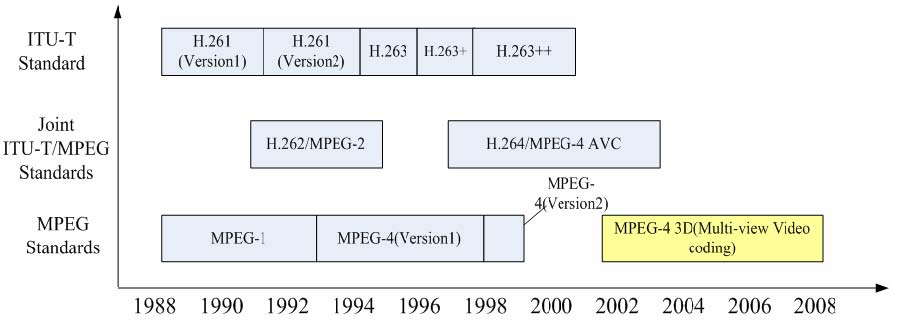
\includegraphics[width=\textwidth]{codecroadmap.png}
\caption{MPEG、VCEG、JVT视频编解码标准的发展}
\label{fig:codecroadmap}
\end{center}
\end{figure}

在2001年6月,经过评估发现,H.26L编码技术基本能够满足MPEG的标准需求,因此MPEG与VCEG的成员共同成立了一个新的工作组JVT(Joint Video Team),来推动和管理H.26L的最后标准化开发,并在2003年形成了视频标准,同时被MPEG和VCEG采纳:MPEG将其定为MEEG-4 part 10,VCEG将其定为H.264。MPEG和VCEG制定的主要标准见。H.264/MPEG-4 part 10标准称为高级视频编码(AVC:Advanced Video Coding),扩展性较好,用于3D视频的多视点视频编解码(MVC:Multi-view Video Coding)就是其一个扩展。MPEG与VCEG及JVT制定的主要视频标准如图\ref{fig:codecroadmap}所示。

\section{已有研究}
\label{sec:previouswork}

%MVC相关工作

在Multi-view Video Coding方向的研究在很久前就开始了。3D视频的一个特点是:传输给用户的各个视角的视频描述的是同一个场景。各个视角的视频在统计意义上的相关性很大,这些相关性就可以用来做预测,如图\ref{fig:mvcpredstruct}所示\footnote{http://mpeg.chiariglione.org/technologies/mpeg-4/mp04-mvc/image004.jpg}。综合利用时间序列以及视角间的图像预测结构,能够极大地提高编码效率\cite{merkle2005statistical}\cite{kaup2006analysis}。\onlinecite{magnor2003multi}中提及了多视点图像编码的一些前沿研究。
\begin{figure}[htbp]
\begin{center}
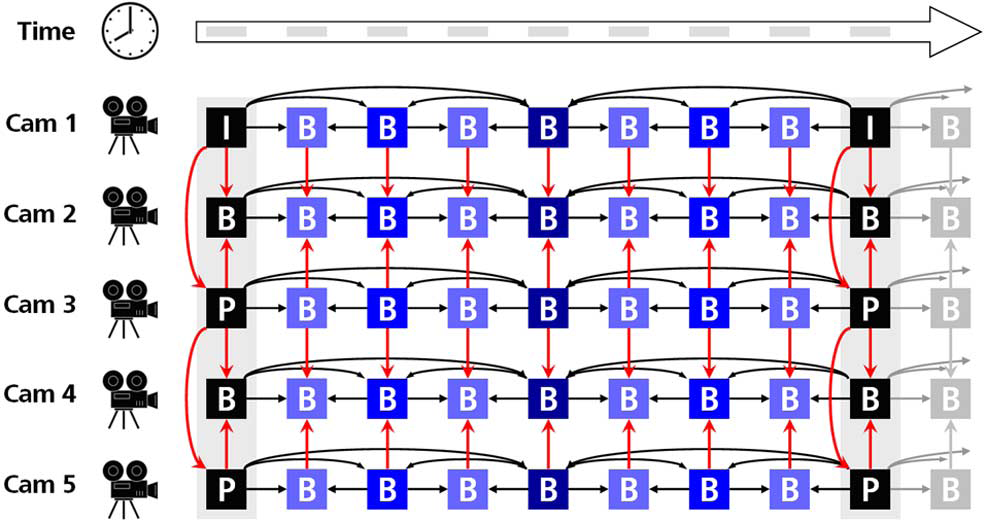
\includegraphics[width=\textwidth]{mvcpredstruct.png}
\caption{MVC的时间和视角间预测结构}
\label{fig:mvcpredstruct}
\end{center}
\end{figure}

对于视角间和时间序列上的图像预测结构,有不少文献提出了不同的方法。其中,H.264/AVC时间和视角间预测的基于B帧的算法\cite{kaup2006analysis}在MPEG标准测试下性能表现最好\cite{flierl2007motion}\cite{merkle2006efficient}\cite{mueller2006multi}\cite{merkle2007efficient}。在实验中,各种指标都显示MVC远远超越了独立压缩每个视角视频的方法。不过,能够获得的性能提升对参数有一定依赖,如相机间距、帧率、内容复杂度(运动和纹理)等属性。对于一些数据集,信噪比峰值(PSNR)的增益在0.5dB以下,而最大的增益能达到3dB。

这个方法在提高视频编码压缩率的同时,增加了编解码的复杂度,要求处理更大量的数据和进行更多的计算。对于MVC编解码的研究大多使用参考软件JMVC进行\footnote{由Heiko Schwarz、Tobias Hinz、Karsten Suehring等人开发。}。参考软件的编写比较注重对应多视点视频编码的原理,对于学习MVC编解码很有帮助,但也因此损失了极大的性能。在实验所使用的机器上对720$\times$576的两路视频进行编码,19帧需要大约半个小时,这远远不够实际应用的需求。诺基亚研究中心(Nokia Research Center)针对其运行Maemo的平台开发了一款MVC实时解码器\footnote{http://research.nokia.com/research/mobile3D},针对单核心做了不少优化。由于其主要利用汇编优化,而处理器并不是x86兼容的,所以不易移植到PC上。

至此,我们认为有必要进行一个能够在PC上进行两路到更多路MVC视频的解码器,进行客户端的实时解码。这样的解码器是3D视频应用普及的一个重要前提。

由于MVC是H.264/AVC的一个扩展,所以我们首先想到H.264的并行编解码问题。这个方向近几年有一些文献:\onlinecite{li2005design}提出的算法使用一个处理器进行动量估计以外的运算,其余处理器进行运动向量的估计。\onlinecite{seitner2007macroblock}做了H.264解码器的宏块并行分析,\onlinecite{mesa2009scalability}给出了H.264解码器宏块并行算法。而更进一步针对多视点视频的并行解码的研究相对较少:\onlinecite{yang2006parallel}提出了一种超空间(hyper-space)的方法,\onlinecite{ugur2007parallel}通过对参考帧施加一定限制条件使得解码器等待参考帧传入的时间大幅降低,从而提升并行解码速度。

%庞一等 论文
庞一等在2009年提出了一种多核架构上并行处理多视点视频的启发式调度框架\cite{pang2009framework}。不同于以往的帧并行或宏块并行的研究,提出了通过优化解码任务调度来提高解码器并行性能的观点,并通过实验证明性能的大幅提升。该方法对多视点视频的调度如图\ref{fig:gopschedulinginmvc}所示,通过重新安排帧解码顺序,最小化多路视频解码时因为等待参考帧传入和其解码结果的等待时间,从而加快解码速度。
\begin{figure}[htbp]
\begin{center}
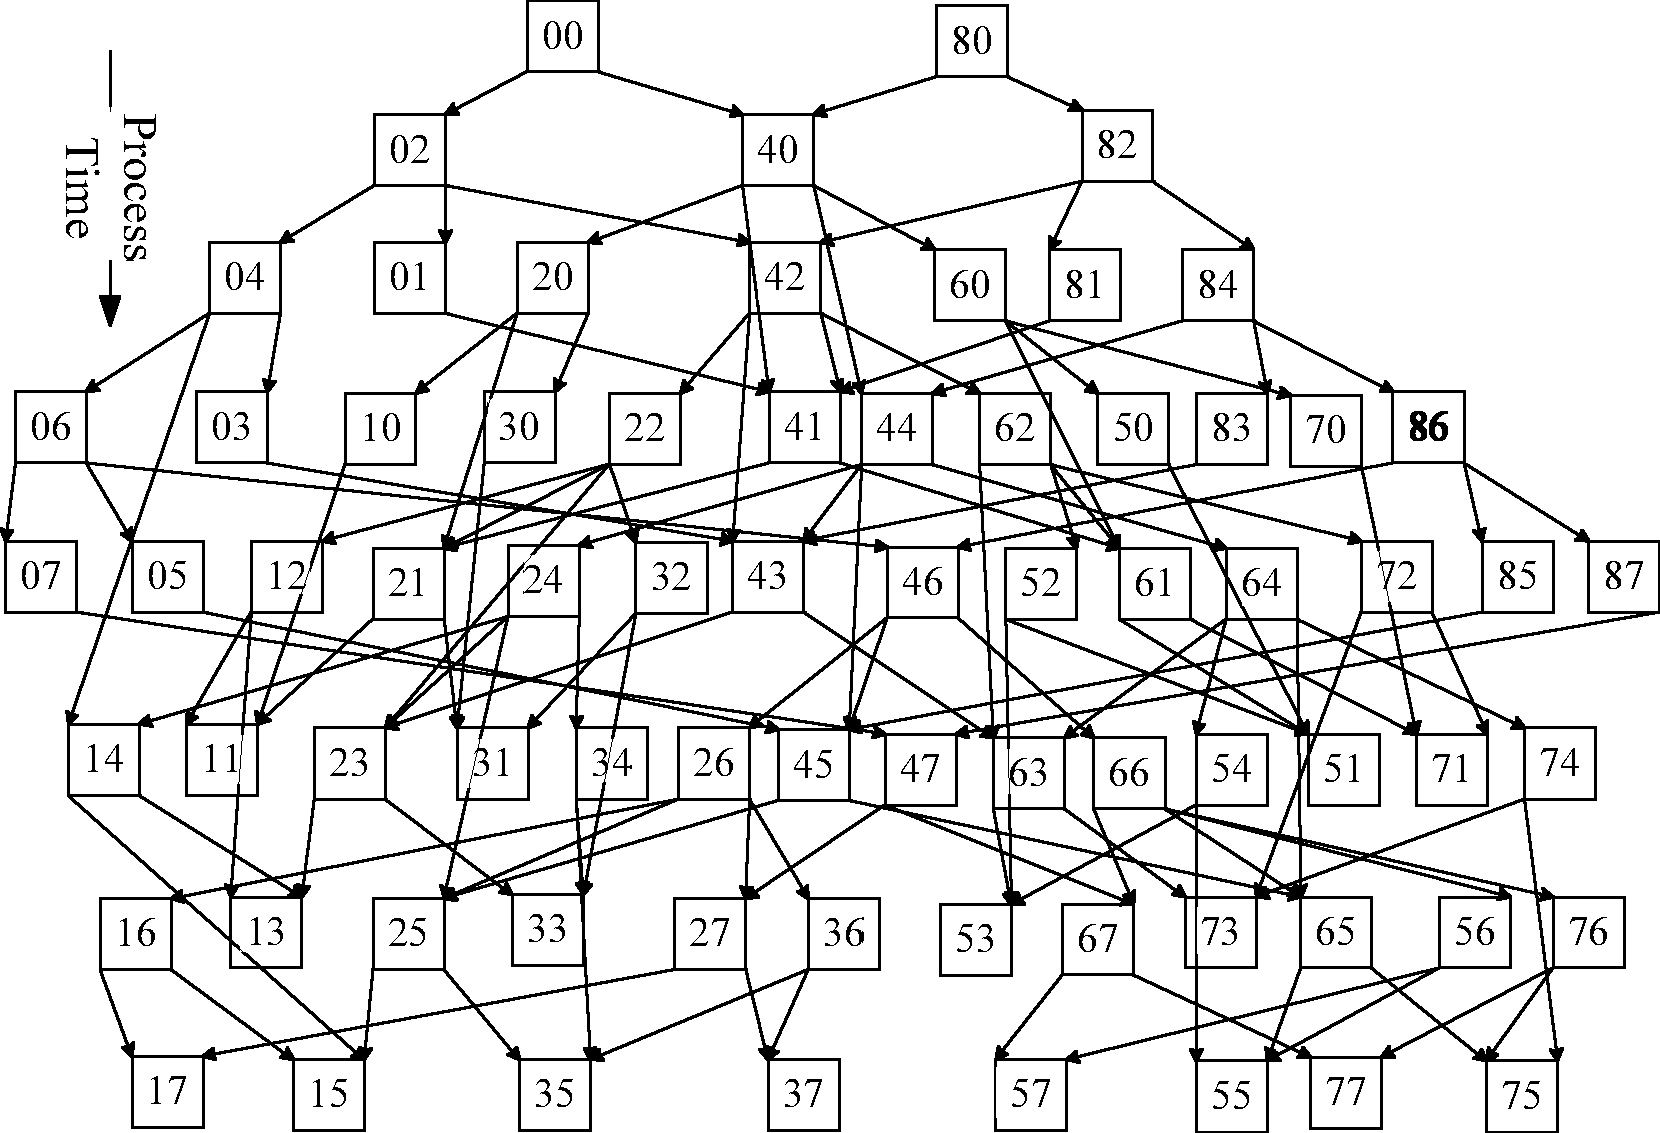
\includegraphics[width=\textwidth]{gopschedulinginmvc.png}
\caption{多视点视频种的GOP调度}
\label{fig:gopschedulinginmvc}
\end{center}
\end{figure}


%MVC Decoder工作
在此基础上,我们已经实现了一个成型的多视点视频编解码系统,包括编码器和解码器。编码器将若干YUV格式的视频编码为一个MVC视频。解码器将一个MVC视频解码为N个独立的YUV视频,N为该MVC视频包含的视角数量。编解码结果符合MVC的标准\cite{iso2009mvc}。

在第\ref{cha:decoderprincipleandrealization}章中将进一步介绍解码器部分。

\section{本文的任务}
\label{sec:workbrief}

目前已有的MVC Decoder工程速度较慢,不能满足实时解码播放的要求。本文主要通过针对单核和多核结构的优化,是现有的MVC解码器能够在CPU上做到至少两路分辨率为720$\times$576的视频的实时解码。

此外,由于MVC视频的标准尚未确定,硬件也尚未普及,还没有一种播放器能够支持各种硬件平台上的MVC视频播放。我们的实验环境有Bolod的3D平板电视和nVidia的3D Vision眼镜套装,为了实现一个从采集到播放的完整系统,除了解码器的优化以外,我还需要设计实现一个3D播放器,让用户能够看到三维的播放效果。

\section{本文的结构}
\label{sec:thesisstructure}

本文第\ref{cha:decoderprincipleandrealization}章介绍需要优化的多视点视频解码器的原理和实现。第\ref{cha:optapproach}章说明我进行解码器性能优化的基本思路。第\ref{cha:singlecoreopt}章和第\ref{cha:parallelopt}章分别详述单核心性能优化和多核处理的并行优化过程。第\ref{cha:optresultandanalysis}章介绍实验结果并进行了一定的分析。第\ref{cha:conclusionandforesight}章总结优化工作并对下一步的工作有所展望。

同时进行的3D播放器设计与实现部分与解码器优化不相关,所以不列在章节中,单独作为附录\ref{cha:3Dplayerdesignandrealization}附在正文之后。
% 
%%% Local Variables: 
%%% mode: latex
%%% TeX-master: t
%%% End: 

\chapter{MVC解码器原理与实现}
\label{cha:decoderprincipleandrealization}

%参见胡伟栋论文和张凤研论文
自2006年起,胡伟栋等开始着手编写一套视频编解码系统。至2010年初基本完成,编解码的过程基本符合MVC标准\cite{iso2009mvc}的描述。编写过程中,主要参考了《H.264 and MPEG-4 video compression, video coding for next-generation multimedia》\cite{richardson2003h}、T264项目\footnote{\href{http://sourceforge.net/projects/t264/}{http://sourceforge.net/projects/t264/}}和JMVC参考软件。代码参考了JMVC的框架设置。

\section{参考软件JMVC介绍}
\label{sec:introtojmvc}
JVT在发布MVC草案的同时还发布了MVC编解码的参考软件JMVM(Joint Multi-view Video Model)。MVC标准确立之后,JMVM改名为JMVC(Joint Multi-view Video Coding),陆续有新版本发布。我们的编解码器起初参考的是JMVC 4.2版,今年由于新发布的JMVC 7.2编解码结果与旧版并不兼容,我们又针对新版做了更正。

JMVC包括以下几个工程:
\begin{itemize}
\item H264AVCCommonLibStatic
\item H264AVCDecoderLibStatic
\item H264AVCEncoderLibStatic
\item H264AVCVideoIoLibStatic
\item MVCBitStreamAssembler
\item MVCBitStreamExtractor
\item DownConvertStatic
\item PSNRStatic
\item H264AVCDecoderLibTestStatic
\item H264AVCEncoderLibTestStatic
\end{itemize}

其中,DownConvertStatic是为了前向兼容;PSNRStatic是进行编码质量分析,与MVC编解码实现无关,不做介绍。

H264AVCCommonLibStatic包含编解码时都需要的一些函数,例如对读取一帧的属性、各类Filter函数、量化与反量化函数、宏块的变换与反变换操作等等。H264AVCDecoderLibStatic就是解码器的函数库,H264AVCEncoderLibStatic则是编码器函数库。H264AVCVideoIoLibStatic是进行视频文件读写操作的函数库。

由于MVC视频文件可能包含多路H.264视频,所以需要对码流进行打包,MVCBitStreamAssembler就是这个模块;相应的,MVCBitStreamExtractor就是从码流中抽取各路视频的模块。

除了函数库之外,JMVC还提供了两个工程演示调用库函数进行MVC编码和解码的过程,分别在H264AVCEncoderLibTestStatic和H264AVCDecoderLibTestStatic中。

\begin{figure}[htbp]
\begin{center}
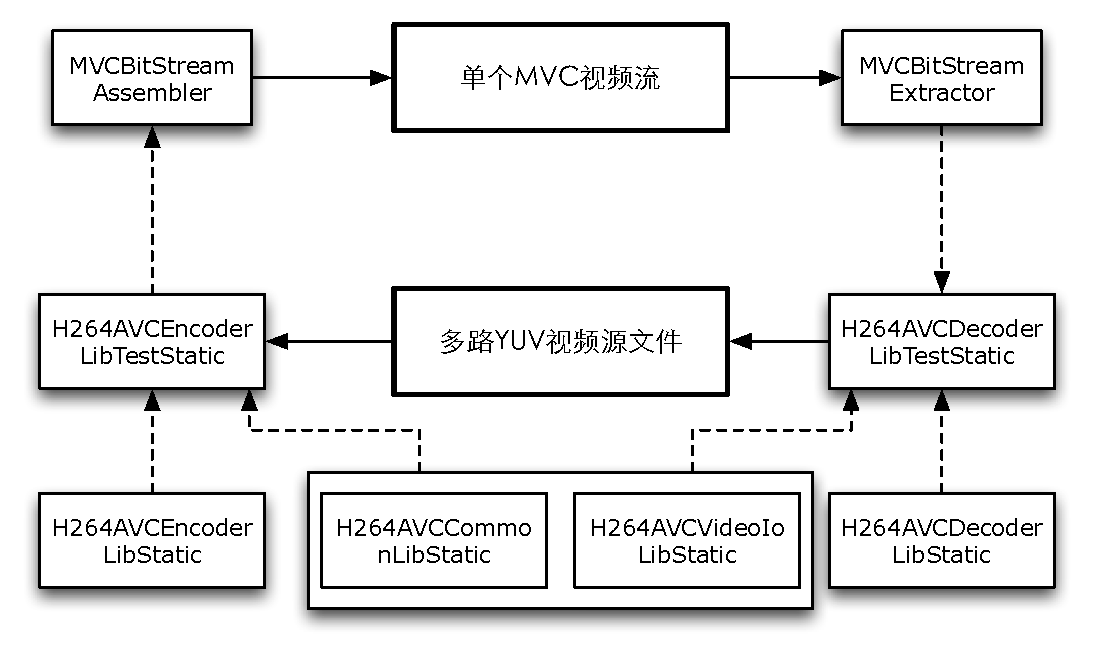
\includegraphics[width=\textwidth]{JMVCstructure}
\caption{JMVC编解码框架}
\label{fig:JMVCstructure}
\end{center}
\end{figure}

利用JMVC进行编解码的框架如图\ref{fig:JMVCstructure}所示。

编码器的输入为若干路YUV视频,一般是同一场景从若干不同角度拍摄的视频,有相同的分辨率并且经过时间同步和校准。YUV文件要求是4:2:0格式,每$2\times2=4$个像素由一个$2\times2$的亮度矩阵和两个$1\times1$的色度矩阵。亮度矩阵顾名思义表示了4个像素的亮度,两个色度矩阵表示像素红蓝两色的平均色度,如图\ref{fig:Barn-yuv}所示。
在编解码器开发期间,庞一、胡伟栋、张凤研等对编解码在帧级别的并行性进行了深入研究\cite{pang2009adaptive,yi2008parallelized},并在编码器和解码器中都采用了帧并行的算法。

\begin{figure}[htbp]
\begin{center}
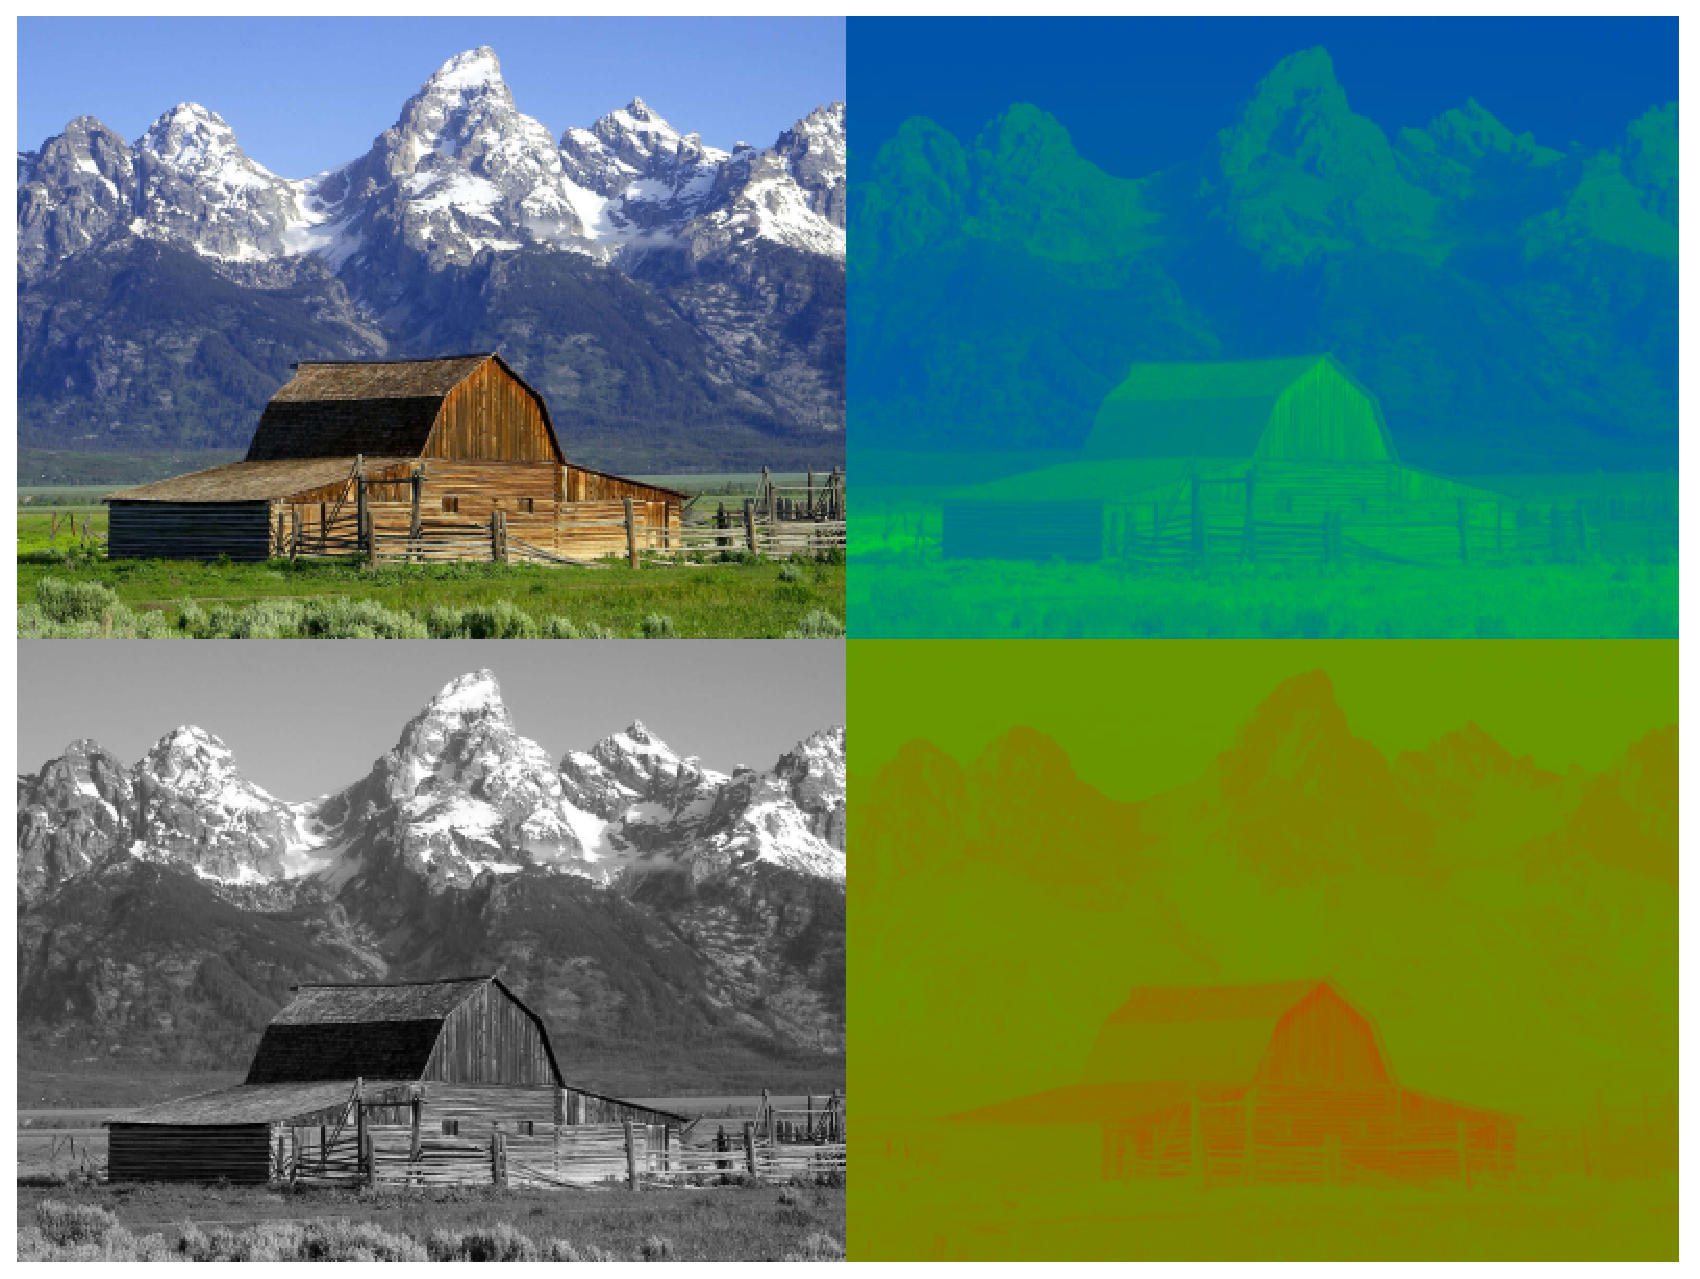
\includegraphics[scale=0.4]{Barn-yuv.eps}
\caption{原始图像(左上)和其Y'(左下)、U(右上)、V(右下)分量}
\label{fig:Barn-yuv}
\end{center}
\end{figure}

\section{自主开发的MVC解码器}
\label{sec:mvcdecoder}
%TODO 解码流程图
%TODO 解码器行为描述
%
%
% %%% 其它部分
% \backmatter
% % 插图索引
% \listoffigures
% % 表格索引
% \listoftables
% % 公式索引
% \listofequations
%
%
% % 参考文献
% \bibliographystyle{thubib}
% \bibliography{ref/refs}
%
%
% % 致谢
% 
%%% Local Variables:
%%% mode: latex
%%% TeX-master: "../main"
%%% End:

\begin{ack}
  ���ĸ�л��ʦ xxx ���ں�����ϵ xxx �����ڶԱ��˵ľ���ָ�������ǵ��Դ����̽�ʹ
  ���������档

  ��������ʡ����ѧԺ��ѧϵ���оŸ��µĺ����о��ڼ䣬���� xxx ��������ָ�����������
  ʤ�м�����л xx ʵ�������� xx ���ڣ��Լ�ʵ����ȫ����ʦ��ͬѧ�ǵ����������֧
  �֣���������ɹ�����Ȼ��ѧ�����������ش���л��

  ��л \thuthesis�����Ĵ������ҵ�����д���������������࣬���ҵ����ĸ�ʽ����Ư����
  ���ࡣ

  ����ѧλ���ĵ���л��������ҳ��˶ʿ����ʿѧλ���IJ���ҳ�����Ա��ƿ��Զ�дһЩ��
  �о�����дһЩ��
\end{ack}

%
% % 附录
% \begin{appendix}
% %%% Local Variables: 
%%% mode: latex
%%% TeX-master: "../main"
%%% End: 

%\chapter{外文资料的原文}
%\label{cha:engorg}
%
%\section{Abstract}
%
%Research efforts on 3DTV technology have been strengthened worldwide recently, covering the whole media processing chain from capture to display. Different 3DTV systems rely on different 3-D scene representations that integrate various types of data. Efficient coding of these data is crucial for the success of 3DTV. Compression of pixel-type data including stereo video, multiview video, and associated depth or disparity maps extends available principles of classical video coding. Powerful algorithms and open international standards for multiview video coding and coding of video plus depth data are available and under development, which will provide the basis for introduction of various 3DTV systems and services in the near future. Compression of 3-D mesh models has also reached a high level of maturity. For static geometry, a variety of powerful algorithms are available to efficiently compress vertices and connectivity. Compression of dynamic 3-D geometry is currently a more active field of research. Temporal prediction is an important mechanism to remove redundancy from animated 3-D mesh sequences. Error resilience is important for transmission of data over error prone channels, and multiple description coding (MDC) is a suitable way to protect data. MDC of still images and 2-D video has already been widely studied, whereas multiview video and 3-D meshes have been addressed only recently. Intellectual property protection of 3-D data by watermarking is a pioneering research area as well. The 3-D watermarking methods in the literature are classified into three groups, considering the dimensions of the main components of scene representations and the resulting components after applying the algorithm. In general, 3DTV coding technology is maturating. Systems and services may enter the market in the near future. However, the research area is relatively young compared to coding of other types of media. Therefore, there is still a lot of room for improvement and new development of algorithms.
%
%\section{Introduction}
%
%Extending visual sensation to the third dimension has been investigated over decades. However, significant consumer mass markets haven't developed yet. 3-D video is established in niche markets, including professional applications (e.g., scientific visualization, medicine) and entertainment (IMAX cinemas, 3-D gaming). In recent years, research efforts have been strengthened worldwide to remove technological obstacles that encumber wider success of 3-D video applications \onlinecite{smolic20063d, onural2004overview, smolic20043dav, smolic2005interactive, onural2006assessment}. Significant improvements have been achieved for all components of the processing chain, from acquisition and signal processing, over 3-D scene representation, coding and transmission, to rendering and 3-D display. Very likely various 3-D video systems, components, applications and services will enter the market in the near future.
%
%Overviews of the state-of-the-art of technology for 3-D video are given in different papers of this Special Issue, each focusing on a specific component of the processing chain. This paper is devoted to coding. Various 3-D scene representation formats are used in different 3-D video systems and applications as de- scribed in \onlinecite{alatan2007scene}. These formats integrate various types of data, such as multiview video, and geometry data in form of depth or 3-D meshes. In general, 3-D video results in a tremendous amount of data that needs to be transmitted, stored or watermarked. Therefore, efficient compression is a key condition for the success of 3-D video. There is also a strong necessity for developing robust 3-D watermarking techniques, which protect the ownership rights. Further, the availability of open international standards is in general an important enabling factor for the development of markets in the media business. ISO/IEC JTC1/SC29/WG11 (Moving Picture Experts Group—MPEG) is one of the international standardization bodies that play an important role in digital media standardization. Therefore, this paper highlights MPEG standards for the different data as available and under development.
%
%The following section gives an overview of coding of multiview video, depth and associated data, with focus on avail- able and emerging MPEG standards. Section III is devoted to compression of static and dynamic 3-D mesh data as used for 3-D video representations as well as for 3-D computer graphics. Error resilience and multiple description coding (MDC) for 3-D is outlined in Section IV. Then, Section V elaborates on protection of 3-D content using watermarking. Finally, Section VI summarizes and concludes the paper.
%
%\section{Coding of Multiview Video, Depth, and Associated Data}
%
%Many 3DTV systems are based on scenarios, where a 3-D scene is captured by a number of cameras (see e.g., \onlinecite{tanimoto2004free, fujii2002free, matsuyama2004real, hamaguchi2003real, carranza2003free, wurmlin20033d, wurmlin20043d, matusik20043d}). The simplest case is classical stereo video with two videos. More advanced systems apply 8, 16, and more cameras. Some systems additionally apply per sample depth data that can also be treated as video signals. This section gives an overview of compression algorithms and standards for such data. An early overview of this research area can be found in \onlinecite{shum2003survey}. Depending on the degree of common content, shared by a subset of the cameras, a coding gain can be achieved in comparison to single-view coding. In multiview coding, correlations between adjacent cameras are exploited in addition to temporal correlations within each sequence. Therefore, multiview coding adds an- other compression dimension on top of single-view coding: the inter-view direction.
%
%\subsection{Conventional Stereo Video Coding}
%Stereo view is the most important special case of multiview with views. Compression of conventional stereo video has been studied for a long time and the corresponding standards are available. A conventional stereo pair consists of two images showing the same scene from two slightly different viewpoints corresponding to the distance of human eyes. The images are in general very similar, which makes them well suited for compression, e.g., with one image predicting the other. For instance one of them can be compressed without reference to the other stereo image. Then, the second image can be predicted from the already encoded one, just like temporally related images can be motion-compensated in video compression.
%
%The samples of both images correspond to each other through the 3-D geometry of the scene and camera properties, including positions and internal camera parameters such as the focal length. The displacement or disparity of each sample in one image with respect to the other is equivalent to a dense motion field in between two consecutive images of a video sequence. Therefore, it is justified to use the same principles of motion estimation and motion compensation for disparity estimation and disparity compensation for image prediction and then to only encode the prediction error or residual further.
%
%Nevertheless, some specific differences between motion compensation and disparity compensation need to be considered. The statistics of disparity vector fields is different from the statistics of motion vector fields. Disparities are biased and relatively large. Zero disparity means a very large depth of the corresponding point in 3D, while 3-D points close to the camera may have very large disparity values. This may require adjustments of entropy coding of the disparity vectors. In general temporally adjacent images of a video sequence tend to be more similar than views of a stereo pair at practical frame rates. Disocclusion effects, i.e., content that is visible in one image is occluded in the other and can therefore not be predicted, are on average more evident in a stereo pair than in between two temporally adjacent video images. Further, specific differences in a stereo pair may come from incorrect white and colour balance but also due to scene lighting and surface reflectance effects.
%
%\begin{figure}[htbp]
%\begin{center}
%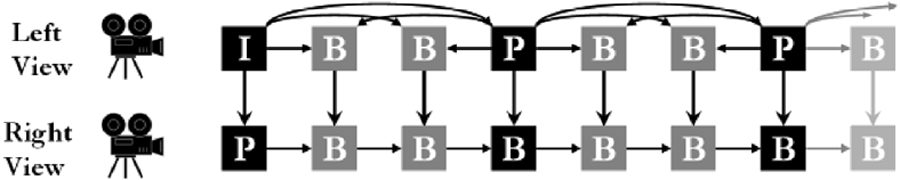
\includegraphics[width=0.8\textwidth]{predh262.png}
%\caption{Illustration of prediction in H.262/MPEG-2 Video multiview profile}
%\label{fig:predh262}
%\end{center}
%\end{figure}
%
%
%The combination of inter-view and temporal prediction is the basic principle for efficient compression of conventional stereo video. A corresponding standard specification has already been defined in ITU-T Rec. H.262/ISO/IEC 13818-2 MPEG-2 Video, the Multiview Profile \onlinecite{haskell1997digital, itu1994mpeg2}, as illustrated in Fig. \ref{fig:predh262}. The left eye view is encoded without reference to the right eye view, using standard MPEG-2. This ensures backward compatibility with Main Profile of H.262/MPEG-2 Video, since it is possible to decode the left eye view bit stream and to display 2-D video. For the right eye view, inter-view prediction is allowed in addition to temporal prediction.
%
%However, the gain in compression efficiency compared to independent encoding of both video streams is rather limited. This is mainly due to the fact that temporal prediction already provides very good performance. Typically, if temporal prediction is efficient for a certain image (e.g., B-pictures for right view in Fig. \ref{fig:predh262}) then additional inter-view prediction does not increase the coding performance significantly. Temporal neighbouring images are typically on average more similar than spatially neighbouring images.
%
%For images that are coded as I-pictures, i.e., without reference to other temporally adjacent images in the video sequence, a significant gain can be achieved by inter-view prediction. Typically every 0.5–1 s such I-pictures are inserted into a video stream to enable random access and error robustness. In Fig. \ref{fig:predh262}, the left-hand side picture of the left view is encoded as I-picture. The corresponding left-hand side picture of the right view would also be encoded as I-picture for random access when in- dependently encoding both video streams. However, in H.262/ MPEG-2 Video multiview coding, inter-view prediction can be applied, resulting in a significant increase of compression efficiency compared to coding this picture as I-picture.
%
%Research on compression of conventional stereo video has continued into several directions, including for instance optimum joined bit allocation for both channels, or abandoning backward compatibility to design more efficient inter-view prediction structures. Algorithms have been based on more up-to-date video codecs such as H.263\onlinecite{itu1995h263}, MPEG-4 Visual\onlinecite{itu1999mpeg4}, or H.264/AVC\onlinecite{sun2005stereo, wiegand2003overview, itu2003h264}. However, none of the developments including the original Multiview profile have reached commercial relevance so far, since the application of stereo video did not develop into a relevant mass market yet.
%
%\subsection{Compression of Video Plus Depth Data}
%
%An alternative to classical stereo video as described in the previous section is to transmit a video signal and a per sample depth map. From the video and depth information, a stereo pair can be rendered at the decoder \onlinecite{fehn2002evolutionary, fehn20043d}. This extends the functionality since it enables head motion parallax viewing if the user’s head motion is tracked. Additionally, this format is interesting from compression efficiency point of view. Per sample depth data can be regarded as a monochromatic, luminance-only video signal. The depth is restricted to a range between two extremes $Z_{near}$ and $Z_{far}$ indicating the minimum and maximum distance of the corresponding 3-D point from the camera respectively. The depth range is linearly quantized with 8 bit, i.e., the closest point is associated with the value 255 and the most distant point is associated with the value 0. With that, the depth map is specified, resulting in a grey scale image. These grey scale images can be fed into the luminance channel of a video signal and the chrominance can be set to a constant value. The resulting standard video signal can then be processed by any state-of-the-art video codec.
%
%Results from the European ATTEST project \onlinecite{fehn2002evolutionary} have shown that depth data can be very efficiently compressed this way. Several state-of-the-art video codecs have been tested (MPEG-2, MPEG-4, H.264/AVC). A course estimate indicates that 10\%–20\% of the bit rate which is necessary to encode the colour video is sufficient to encode the depth at good quality. This is due to the specific statistics of depth data, being on average smoother and less structured that colour data.
%
%Based on these observations, a new backward compatible (with respect to classical DVB) approach for 3DTV was developed in the ATTEST project. It uses a layered bit stream syntax. The base layer is a conventional 2-D colour video encoded using MPEG-2. This base layer can be processed by any existing MPEG-2 decoder providing backward compatibility. Additionally the bit stream contains an advanced layer carrying the encoded depth information. Advanced systems may access this layer to decode the depth stream and then generate a stereo pair to be displayed stereoscopically by view interpolation.
%
%This concept is highly interesting due to the backward compatibility, compression efficiency and extended functionality compared to conventional stereo video. Moreover, it does not introduce any specific coding algorithms. It is only necessary to specify high-level syntax that allows a decoder to interpret 2 incoming video streams correctly as colour and depth. Additionally information about depth range($Z_{near}$ and $Z_{far}$) needs to be transmitted. Therefore, MPEG specified a corresponding container format “ISO/IEC 23002-3 Representation of Auxiliary Video and Supplemental Information,” also known as MPEG-3 Part 3, for video plus depth data \onlinecite{iso2007rep, iso2007fdam}. Moreover, H.264/AVC contains an option to convey the depth images through its auxiliary picture syntax. Here, the video codec for the colour video signal and associated depth video signal are both H.264/AVC. This approach is backwards compatible with any existing deployment of H.264/AVC.
%
%A general problem of the video plus depth format is content creation, i.e., the generation of depth information. Cameras that automatically capture per pixel depth with the video are available and are being further enhanced, but the quality of the captured depth fields is currently still limited. Algorithms for depth estimation have been studied extensively in computer vision literature and powerful solutions are available. However, it always remains an estimation that can only be solved up to a residual error probability. Estimation errors influence the quality of rendered views. A fully automatic, accurate and reliable depth capturing system is still to be developed. User-assisted content generation is an option for specific applications. Even having perfect depth available, artifacts may occur in rendered views due to disocclusion. This effect increases with the distance of the virtual view from the original camera position. Additional occlusion layers (layered depth video as extension of layered depth images \onlinecite{shade1998layered}) or extension to multiview video plus depth \onlinecite{zitnick2004high, kauff2007depth}, help to minimize these problems at the cost of increased data rate and complexity.
%
%\subsection{Multiview Video Coding}
%
%\begin{figure}[htbp]
%\begin{center}
%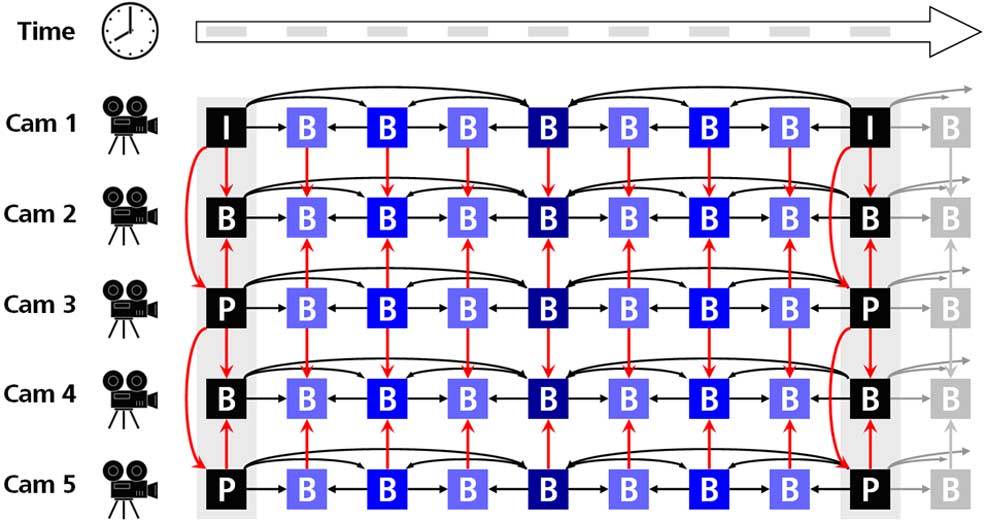
\includegraphics[width=0.8\textwidth]{tempinterpred.jpg}
%\caption{Temporal/inter-view prediction structure for MVC.}
%\label{fig:tempinterpred}
%\end{center}
%\end{figure}
%
%A common element of many 3DTV systems is the use of multiple views of the same scene that have to be transmitted to the user. The straight-forward solution for this would be to encode all video signals independently using a state-of-the-art video codec such as H.264/AVC. However, multiview video contains a large amount of inter-view statistical dependencies, since all cameras capture the same scene from different view-points. These can be exploited for combined temporal/inter-view prediction, as illustrated in Fig. \ref{fig:tempinterpred}. Images are not only predicted from temporally neighbouring images but also from corresponding images in adjacent views. Statistical evaluations have shown that significant gain can be expected from such combined temporal/inter-view prediction \onlinecite{merkle2005statistical, kaup2006analysis}. Pioneering work on multiview image coding is reported in \onlinecite{magnor2000data, magnor2003multi}.
%
%Several research groups addressed multiview video coding (MVC) and developed dedicated inter-view/temporal prediction structures to efficiently exploit all statistical dependencies within the multiview video data sets (see e.g., \onlinecite{oh12542multi, cheng2006multi, yang2006hyper, vetro2004coding, kalva2006design, socek2006permutation, kalva2006challenges, bilen2006multi}. Among those, algorithms that are based on hierarchical B-pictures \onlinecite{schwarz2006analysis} as supported by H.264/AVC syntax in temporal and inter-view dimension (Fig. \ref{fig:tempinterpred}) proved best performance in exhaustive experiments conducted in the context of MPEG standardization \onlinecite{flierl2007motion, merkle2006efficient, mueller2006multi, merkle2007efficient}. In these experiments, it has been shown by objective and subjective measurements that dedicated MVC outperforms independent encoding of the multiple video streams significantly. However, the achievable gain strongly depends on the content and its properties such as camera distance, frame rate and complexity of the content (motion, texture). For some data sets the peak signal-to-noise ratio (PSNR )gain was reported as 0.5 dB and below. Maximum reported gains were up to 3dB.
%
%A drawback of combined temporal/inter-view prediction as illustrated in Fig. \ref{fig:tempinterpred} is the complexity. This includes computational complexity, memory requirements and delay. In \onlinecite{merkle2007efficient, merkle2007coding}, it has been shown that the complexity can be significantly decreased without sacrificing much coding efficiency. Inter-view prediction is restricted here to the key pictures that would be treated as I-pictures in independent encoding of the views (e.g., time and in Fig. \ref{fig:tempinterpred}). Most of the coding gain of MVC comes from inter-view prediction of these pictures that do not use temporal prediction for temporal random access reasons. Omitting inter-view prediction for pictures that have a temporal reference does not cost much coding efficiency whereas it decreases complexity significantly.
%
%In addition to combined temporal/inter-view prediction, specific MVC algorithms have been proposed. The basic idea of depth/disparity-based view interpolation prediction \onlinecite{martinian2006view, kitahara2006multi, martinian2006extensions} is to estimate depth or disparity either at the encoder (this requires overhead for sending the depth/disparity) or the decoder, and to perform view interpolation or 3-D warping for prediction. However, the gains reported so far are marginal. Only for very few test data sets with very close camera settings such view interpolation prediction provides a gain of up to 5\% bit rate saving at the same visual quality. Further investigations are needed to optimize the performance.
%
%Further, illumination and color inconsistencies affect the exploitation of inter-view statistical dependencies. Usually such effects should be minimized by proper setting of the conditions, however, an MVC algorithm should also be able to cope with this as well, since proper white and color balancing of the input can not be guaranteed. Also, the illumination (spotlights, shadows, etc.) varies largely over the multiview images due to the lighting conditions. These problems might be handled by proper illumination and color compensation as proposed in \onlinecite{kim2006results} and \onlinecite{lee2006results}. The basic idea is to modify the motion compensation on macroblock level. Before subtracting the pixel values of the block to be encoded and the reference block, the mean of each is compensated from the corresponding pixel values. This assumes locally constant illumination and color variations, which is an appropriate model trading-off accuracy and complexity. Gains of up to 0.7 dB have been reported for some test data using illumination compensation. However, this strongly depends on the test data and in some cases the gain is negligible or there is none at all. On average over all test data sets a bit rate reduction of 5\% was reported for the same visual quality.
%
%An alternative to illumination compensation on macroblock level integrated into the encoding process, also an appropriate preprocessing can be applied, prior to encoding. Algorithms for illumination correction are well-known in image and video processing. Then the corrected data can be passed to a standard encoder. The big advantage of such an approach is that no changes are necessary to the encoder, decoder and bit stream syntax. A preliminary investigation in this direction is presented in \onlinecite{fecker2006improving}, however, results are not complete and performance in comparison to integrated illumination compensation is not clear.
%
%Another research direction is improving disparity estimation, compensation, and coding \onlinecite{lu2009effective}. Mostly disparity is treated equally to motion, however, it is known that the statistical properties of disparity vectors can be quite different compared to those of motion vectors. Disparity estimation has been studied extensively in the computer vision literature. Usually, basic geometric properties and constraints are taken into account. For instance, the search can be done along epipolar lines.
%
%This may lead to better estimates and reduce the complexity. Further, specific disparity coding may improve the efficiency of inter-view prediction. Specific coding modes for MVC such as the inter-view direct mode \onlinecite{guo2006inter} are under investigation.
%
%Combination of scalability with MVC is investigated for in- stance in \onlinecite{garbas20064d, drose2006extending, yang20064, yang2005scalable, ozbek2006scalable}. So far the feature of scalability only comes with decreased compression efficiency. Distributed MVC is investigated for instance in \onlinecite{guo2006distributed}. Also first work on efficient trans- port and delivery taking user interactivity into account has been presented \onlinecite{kurutepe-interactive, kurutepe2006interactive}. Finally, efficient mechanisms for optimum random access, parallel processing and memory management for MVC have been investigated.
%
%Since the results clearly indicate that MVC outperforms independent encoding of the multiple video signals, and there is a clear demand from industry for a corresponding standard, ISO/ MPEG and ITU/VCEG decided developing a dedicated MVC specification \onlinecite{vetro-joint, vetro2006joint}. It will be an extension of H.264/AVC (Amendment 4), which is scheduled to be finalized in 2008. MVC is the main focus of this Special Issue. We therefore refer the reader to the dedicated articles in this volume that contain all details of state-of-the-art MVC technology.
%
%\subsection{Conclusions and Future Research Directions}
%
%Research on coding of stereo video, multiview video and associated depth or disparity data has reached a good level of maturity. Related international standards are available enabling a variety of 3DTV systems and applications. However, compared to coding of other types of media data the scientific field is relatively young, and therefore there is still a lot of room for improvement of algorithms. This includes for instance optimization of MVC and development of new specific coding MVC algorithms. Depth or disparity coding may be improved further by development of dedicated algorithms. Further, there are more complex types of data representations for 3DTV such as layered depth video and multiview video plus depth that provide extended functionality. Efficient coding algorithms for such data are still under investigation. Initial results are reported in \onlinecite{merkle2007efficientmvc} and \onlinecite{merkle2007multi}. Other types of multiview representations are also under investigation often related to specific types of 3-D displays. An example is presented in \onlinecite{saishu2006flatbed}.
%
%%\cleardoublepage

\chapter{外文资料的书面翻译}

\section{摘要}

最近,3D电视技术相关的研究工作在全球范围内都有增加。这些研究覆盖了整个媒体处理流程,从采集到显示无所不包。不同的3D电视系统依靠各种类型数据构成的不同的3D场景表示方式。对这些数据的高效编码对于3D电视的成功至关重要。对双目视频、多视点视频、深度图或视差图中像素类型数据的压缩拓展了已有的经典视频编码的原则。针对多视点视频和视频加深度数据的强大算法和开放的国际标准已经出现并一直有着进展,这为在不久的将来引进各种3D电视系统奠定了基础。对3D网格模型的压缩也达到了高度成熟的程度。对静态的几何体,有多种强大的算法可以有效地压缩顶点和连接数据量。对动态3D几何体的压缩是现在更受关注的研究方向。基于时间的预测是一个重要的对动画3D网格序列去冗余信息的机制。容错性对于在易出错的信道上传输数据十分重要,而多描述编码(MDC)是一种可行的保护数据的方法。对静态图和2D视频的MDC已经得到了广泛的研究,但是对多视点视频和3D网格的MDC最近才刚刚提出。用水印进行3D数据的知识产权保护也是一个前沿的研究方向。3D水印方法方面的文献根据表示场景的主要部分在应用算法前后的维数可以归为三类。总而言之,3D电视编码技术正在走向成熟。相关系统和服务可能在不久的将来进入市场。然而,这个方向的研究相对其他媒体数据的研究而言又很少,所以仍有很大的空间可以改进,有很多新的算法可能被提出。

\section{简介}

将我们的视觉延伸到三维空间在近几十年中一直都在研究,但是大规模的消费市场仍然没有发展起来。3D视频还在小众市场发展,包括专业应用(比如科学数据可视化、医药学等)和娱乐方面(比如IMAX影院、3D游戏等)。近年来,更多的研究精力投向了这个领域,以期能够跨越阻碍3D视频应用得到更广泛成功应用的障碍\cite{smolic20063d, onural2004overview, smolic20043dav, smolic2005interactive, onural2006assessment}。从获得信号、处理信号到3D场景表示、编码、传输,再到渲染和3D显示,整个处理流水线的各个部分都取得了显著的进步。很可能在不久的将来,各种3D视频系统、组件、应用和服务就会进入市场。

这一期中给出了各种尖端3D视频技术的综述,分别针对一个3D视频处理流水线中的一个特定组件。这篇文章介绍编码相关的部分。\onlinecite{alatan2007scene}中介绍了用在不同的3D视频系统和应用中的不同3D场景表示格式在。这些格式整合了各种类型的数据,比如多视点视频、深度或3D网格的几何数据。总的来说,3D视频就意味着有大量的数据需要传输、存储和水印。于是高效的压缩就是3D视频成功与否的一个关键条件。同时对发明一个鲁棒的3D水印技术来保护所有权也有很强的需求。此外,开放的国际标准对市场和相关商业的发展也是一个推动力。ISO/IEC JTC1/SC29/WG11 (Moving Picture Experts Group—MPEG)就是一个在数字媒体标准化中起到重要作用的国际标准化组织。所以,这篇文章关注现有的和正在成形的各种数据的MPEG标准。

接下来的几节分别给出多视点视频、深度和关联数据的编码综述,集中关注已有的和正在成形的MPEG标准。第3节介绍用于3D视频表示以及3D计算机图形学的静态和动态3D网格数据的压缩。容错以及3D视频的多描述编码(MDC)在第4节中介绍。然后在第5节中介绍用水印保护3D内容的方法。最后,第6节概况和总结这篇文章的观点。

\section{多视点视频、深度和关联数据编码}

很多3D电视系统都基于场景,这些3D场景由N个相机获取(见\onlinecite{tanimoto2004free, fujii2002free, matsuyama2004real, hamaguchi2003real, carranza2003free, wurmlin20033d, wurmlin20043d, matusik20043d})。最简单的情形就是经典的两路视频构成的立体视频,更复杂一些的系统用8路、16路或更多路相机获取的视频。有些系统还使用可以当作视频信号的深度信息。这一节综述这类数据的压缩算法和标准。更早对这个研究方向的综述可以参见\onlinecite{shum2003survey}。通过共享内容、共享一些相机,多视点视频比起单视点视频的编码可以一定提升。在多视点视频编码中,除了挖掘单个相机的数据在时间上的关联之外,临近的相机之间的关系也被挖掘出来。于是多视点视频在单视点视频的基础上增加了一个新的压缩维度:视点间的方向。

\subsection{传统立体视频编码}

立体视频是多视点视频中最重要的一个特例,是有N=2个视点的情形。 压缩传统的立体视频已经经过了长时间的研究,相关的标准也已经问世。一个传统的立体对由从两个略微不同的视点(对应人的瞳距)观察同一场景的两幅静态图组成。这两幅图片总的来说极其相似,使得它们很适合压缩,比如从一幅图片预测另一幅。例如,其中一幅可以不参考另一幅而单独压缩,而第二幅图片可以从已经编码的一幅图片来预测,就像视频压缩中的基于时间预测的动态补偿那样。
 
对两幅图片的样本基于场景和相机属性(包括位置和相机内部参数比如焦距)的3D几何各自对应起来。每个样本的位移或视差就等价于一个视频序列中两幅连续图像的dense motion field。于是就可以用运动估计和运动补偿一样的方法去做视差分析和视差补偿,以此实现图像预测,然后就只需要编码预测误差或者进一步的残差即可。

然而,一些特定的动态补偿和视差补偿间的区别需要考虑进来。视差向量场的统计与运动向量场的统计不同。视差是有偏的,而且相对较大。零视差以为着一个点在 3D场景中的深度极大,而一个距离相近很近的3D点会有很大的视差值。这需要对视差向量的熵编码做调整。总的来说,在正常的帧率下,视频序列中在时间上邻近的图像倾向于比立体视频的两个视点的图像更加相似。图像损失(内容在一张图中可见但是在另一张图中不存在,也就无法被预测)平均来说在立体视频中出现得比时间上邻近的两幅图更多。此外,立体图片对中的差别可能来自不正确的白平衡或色彩平衡,也可能来自场景的光照和表面反射效果的差别。 

\begin{figure}[htbp]
\begin{center}
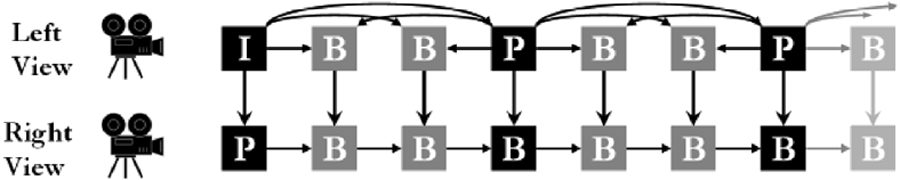
\includegraphics[width=0.8\textwidth]{predh262.png}
\caption{H.262/MPEG-2视频多视点类(multiview profile)的预测示意}
\label{fig:predh262chs}
\end{center}
\end{figure}

视角间和时间上的预测组合是有效压缩传统立体视频的基本方法。对应的标准已经在ITU-T Rec.H.262/ISO/IEC 13818-2 MPEG-2Video, the Multiview Profile\cite{haskell1997digital, itu1994mpeg2}中定义了,如图\ref{fig:predh262chs}所示。左眼视频不参考右眼视频单独编码,使用标准的MPEG-2。这保证了对H.262/MPEG-2的主类(Main Profile)的前向兼容性,因为这样可以解码左眼视频流来显示2D视频。对右眼视频,时间轴预测之外还可以允许做视点间预测。
 
然而,对比分别压缩两个视频流而言,这样的压缩效率提升很有限。这主要是由于基于时间的预测已经达到了很高的性能。特别是当基于时间的预测对于一张特定图像效率不错的时候(比如图\ref{fig:predh262chs}中右眼视频的B帧),那么增加视角间的预测就无法显著提升编码性能了。时间上邻近的图像平均而言一般都比空间上邻近的图像更相似。

对于编码为I帧的图像,也就是说不参考其他视频序列中时间上邻近的帧来编码的帧,加入视角间的预测有明显成效。一般每半秒到一秒时间就会在视频序列中插入这样一个I帧来保证随机访问和容错性。在图\ref{fig:predh262chs}中,左眼序列的最左侧一帧被编码为I帧,当分别编码两个视频序列时,对应的右眼序列中的那一帧也可以编码为I帧。但是在H.262/MPEG-2视频多视点编码中,可以采用视角间预测来达到压缩效率上比编为I帧方式的显著提升。

对于传统立体视频压缩的研究还在各个方向上继续进行着,包括对各个频道的最优码率分配以及放弃前向兼容去设计一个更加有效的视角间预测的结构。相关算法是都是基于更新的视频编码比如H.263\cite{itu1995h263},MPEG-4 Visual\cite{itu1999mpeg4}或H.264/AVC \cite{sun2005stereo, wiegand2003overview, itu2003h264}。但是由于立体视频的应用还没有发展到一个足够大的市场,所有这些进展包括原有的多视点类(Multiview profile)都尚未能商业化。

\subsection{视频加深度数据的压缩}

除了前文描述的经典立体视频外,还有一种传输视频信号的方式——传输一路视频和每个样本的深度图。从视频和深度信息,可以在解码端渲染出一对立体图\cite{fehn2002evolutionary,fehn20043d}。这提供了另一项功能:当用户的头部移动被捕捉到时,能够提供相对应的观察角度的图像。此外,这种格式从压缩效率的角度来看很有价值。深度信息可以被当作单色、仅有明度的视频信号。深度被限制在两个表示对应3D点到摄像机的最小和最大距离的极限距离$Z_{near}$和$Z_{far}$之间。深度范围线性地量子化到8位,也就是最近的点赋值255,最远点赋值为0。这样一来,一张深度图就确定下来了,成为一张灰度图。这些灰阶图可以被插入视频信号的光照信道中,其色彩可以被设定为一个常数。这样获得的标准视频信号就可以用任何先进的视频编码处理了。

欧洲ATTEST的一个项目\cite{fehn2002evolutionary}结果表明深度信息可以用这种方式非常高效地压缩。一些前沿的视频编码参与了测试(MPEG-2, MPEG-4, H.264/AVC)。一项估计显示,只要编码彩色视频信号10\%到20\%的比特率就足以编码高质量的深度信息了。

基于这些观察,这个ATTEST项目提出了一种新的(对比经典的DVB)向前兼容的实现3DTV的方式。它采用一种分层的比特流语法。基层是一个传统的 MPEG-2编码的彩色2D视频。基层可以被任何现有的MPEG-2解码器处理,保证前向兼容性。除此之外,比特流还包含更高一层传输编码后的深度信息。更高级的系统可以访问这一层来解码深度信息,然后通过插值生成一对立体图像来显示。

这种概念由于保证了前向兼容性、压缩率高并且相比传统立体视频功能扩展更多,所以非常有价值。不仅如此,它并不引入一种特定的编码算法。只需要制定一种高层的语法,让解码器能够把输入的两路视频正确地分辨成一路视频和一路深度即可。附加的深度信息($Z_{near}$和$Z_{far}$)需要另外传输。所以MPEG为视频加深度信息制定了一种对应的容器格式 “ISO/IEC 23002-3 Representation of Auxiliary Video and Supplemental Information”,或者称为MPEG-3 Part 3\cite{iso2007rep, iso2007fdam}。此外,H.264/AVC包含一个选项通过辅助的图片语法传输深度图。此处对彩色视频信号和对应的深度视频信号的视频编码都用的是 H.264/AVC。这种方法对任何已部署的H.264/AVC设备都能做到前向兼容。

对视频加深度的格式而言,有一个普遍存在的问题就是深度信息的生成。能够在捕获视频的同时自动获取每个像素深度的摄像机已经问世而且在进一步增强,但是得到的深度场的精度还是很有限。计算机视觉相关的文献中对深度估计的算法有了很深入的研究,强大的解决方案也已经出现。但是这总是一个建立在一定残差误差概率上的估计值。估计的误差会影响渲染出的图像的质量。全自动而且精确的深度获取系统仍然有待开发。对于特定的应用,用户辅助的内容生成可以作为一种选择。即使有了完美的深度图,遮挡也会使渲染出的图像有瑕疵。这些效应在距离原始摄像机位更远的虚拟点上会更加严重。增加一些层(深度视频层作为深度图像层的扩展\cite{shade1998layered})或者扩展到多视点视频加深度\cite{zitnick2004high, kauff2007depth}能够以增加数据量和复杂度为代价,帮助减小这些问题。

\subsection{多视点视频编码}

\begin{figure}[htbp]
\begin{center}
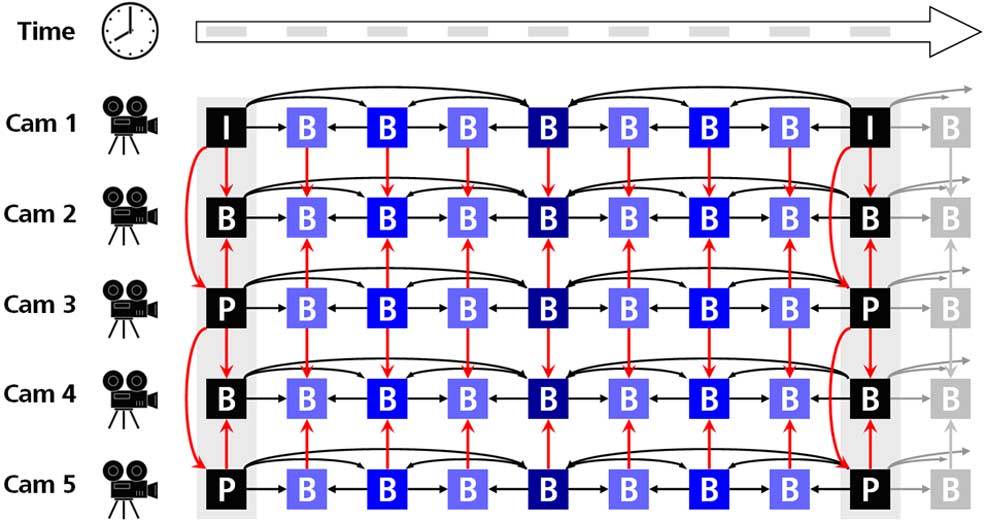
\includegraphics[width=0.8\textwidth]{tempinterpred.jpg}
\caption{MVC的时间和视角间预测结构}
\label{fig:tempinterpredchs}
\end{center}
\end{figure}

3DTV系统的一个共同部分是传输给用户的同一场景不同视角视频的使用。最直接的解决方法就是把所有的视频信号分别用最新的编码方式比如 H.264/AVC编码。但是多视点视频在视角间存在统计意义上很大的相关性,因为每个摄像机捕获的都是不同视角的同一场景的图像。这些相关性可以用来进行时间和视角间预测,如图\ref{fig:tempinterpredchs}所示。图像不仅仅根据时间上临近的图来预测,还根据相邻视角的对应图像预测。统计表明这样的组合式预测能够极大地提高编码效率\cite{merkle2005statistical, kaup2006analysis}。多视点图像编码的前沿研究在\onlinecite{magnor2000data, magnor2003multi}中有报告。

几个研究小组提出了多视点视频(MVC),并且发展了专门的视角间和时间预测的架构来有效地挖掘利用多视点视频数据集中的统计相关性(见\onlinecite{oh12542multi, cheng2006multi, yang2006hyper, vetro2004coding, kalva2006design, socek2006permutation, kalva2006challenges, bilen2006multi})。其中,H.264/AVC时间和视角间预测的语法支持的基于B帧的算法\cite{schwarz2006analysis}在MPEG标准的穷尽测试下被证明是性能最好的\cite{flierl2007motion, merkle2006efficient, mueller2006multi, merkle2007efficient}。在这些实验中,客观和主观的测量都显示MVC极大地超越了独立压缩各个视频。然而,能够获得的提升极其依赖内容和相机间距、帧率、内容复杂度(运动、纹理)等属性。对于一些数据集,信噪比峰值(PSNR)增益在0.5dB以下。最大的增益达到过3dB。

图\ref{fig:tempinterpredchs}中描述的时间和视角间组合预测的一个不足就是其复杂度。包括计算复杂度、内存需求和延迟。在\onlinecite{merkle2007efficient, merkle2007coding}中提到,复杂度在不牺牲多少编码效率的情形下可以极大地降低。视角间预测此时被限制在作为I帧独立编码的关键帧上(例如图\ref{fig:tempinterpredchs}中的$t_0$和$t_8$)。MVC中大部分编码增益来自于这些为了随机访问而不进行视角间预测的帧。忽略有时间预测的帧的视角间预测并不消耗多少编码效率却显著降低复杂度。

在结合时间和视角间预测之外,专门的MVC算法被提了出来。基于深度/视差的视角间插值预测\cite{martinian2006view, kitahara2006multi, martinian2006extensions}的基本思想是在编码(这需要另外传输深度/视差)或解码端估计深度或视差,然后进行视角间插值或者3D扭曲来预测。但是目前得到的增益不高。仅仅对于摄像机参数极其接近的很小一部分数据集,这样的视角间插值预测在同样画质下能节省5\%的比特率。想要优化性能还要做进一步的研究。

不仅如此,光照和色彩的不一致影响了对视角间统计相关性的挖掘。通常这样的效应能被正确的条件设定减小,但是 MVC算法也要能够应对这样的情形,因为输入的白平衡和色彩平衡并不能保证。同样,一定的光照条件下,光照(聚光灯、阴影等)在视角间会有很大的不同。这些问题或许能通过\onlinecite{kim2006results}和\onlinecite{lee2006results}中提出的正确的光照和色彩补偿来解决。基本思想是在宏块级别修改运动补偿。在对待编码帧块和参考块的像素值相减之前,二者的平均值根据对应的像素值做补偿。其中假设了本地的光照和色彩变化是常值,这是个模型的准确率和复杂度之间的权衡。对于一些测试数据,光照补偿获得了0.7dB的增益。但是这个增益极大地依靠测试数据,在一些情况下,增益可以忽略甚至根本不存在。对所有的测试数据集平均下来,相同视觉质量下,能够节省5\%的比特率。

另一种宏块级别的光照补偿可以整合到编码过程中,一个合适的预处理也可以在编码前进行。对图像和视频的光照更正算法广为人知。然后更正过的数据可以被传到一个标准的编码器。这种方法的一大优势是编码器、解码器和码流语法不需要做任何改动。一项这个方向上的前期调研发表在\onlinecite{fecker2006improving}中,但是结果并不完全,性能与整合光照补偿的比较也不清楚。

另一个研究方向是改进视差估计、补偿和编码\cite{lu2009effective}。多数的视差都被当作运动来对待,但是我们知道视差向量的统计属性和运动向量可以完全不同。视差估计在计算机视觉文献中已经被广泛研究。通常,级别的几何属性和约束会考虑进来。比如搜索可以通过沿着核极线(epipolar lines)完成。这可能带来更好的估计和降低复杂度。此外,专门的视差编码或许能提高视角间预测的编码效率。专门的MVC编码模式比如视角间直接模式\cite{guo2006inter}正在研究中。

MVC的扩展性结合正在被研究,比如\onlinecite{garbas20064d, drose2006extending, yang20064, yang2005scalable, ozbek2006scalable}。目前可扩展的功能仅能依靠降低压缩效率。分布式MVC在\onlinecite{guo2006distributed}中被研究。加入用户交互考虑的有效传输在\onlinecite{kurutepe-interactive, kurutepe2006interactive}中初次被讨论。最后,能够随机访问的有效的MVC编码机制、并行处理和内存管理也正在研究中。

由于结果明显表明MVC优于单独编码各路视频信号,业界又显然需要一个对应的标准,ISO/MPEG和ITU/VCEG 决定发展一种专门的MVC标准\cite{vetro-joint, vetro2006joint}。这会是一个H.264/AVC的扩展(第4修正案),这预计在2008年内完工。MVC是这一期特刊的主要关注点。我们因此向读者介绍包含最前沿MVC技术的文章。

\subsection{结论和未来研究方向}

对立体视频、多视点视频和相关深度、视差数据的研究已经有很高的成熟度。相关的国际标准也已经问世,使3DTV系统和应用成为可能。然而,相对于其他类型和媒体数据的编码,这个领域还很年轻,算法还有很大的进步空间。这包括对MVC实力的优化和新的专门的MVC算法的开发。深度和视差编码可能在将来的专门的算法中进一步优化。此外,有更多复杂的3DTV数据结构比如分层的深度视频和多视点视频加深度来提供更多的功能。对这些数据的有效编码算法还在研究之中。初步的结果在\onlinecite{merkle2007efficientmvc}和\onlinecite{merkle2007multi}中有报告。其他多视点描述的类型也在研究中,这往往和特定的一类3D显示器相关。\onlinecite{saishu2006flatbed}中有一个例子。

\begin{center}
\heiti{原文索引}
\end{center}

Smolic A, M{\"u}eller K, Stefanoski N, et al. Coding algorithms for 3DTV—a survey. IEEE transactions on circuits and systems for video technology, 2007, 17(11):1606–1620

%\cleardoublepage
% \end{appendix}
%
% % 个人简历
% \begin{resume}

  \resumeitem{个人简历}

  xxxx 年 xx 月 xx 日出生于 xx 省 xx 县。
  
  xxxx 年 9 月考入 xx 大学 xx 系 xx 专业,xxxx 年 7 月本科毕业并获得 xx 学士学位。
  
  xxxx 年 9 月免试进入 xx 大学 xx 系攻读 xx 学位至今。

  \resumeitem{发表的学术论文} % 发表的和录用的合在一起

  \begin{enumerate}[{[}1{]}]
  \item Yang Y, Ren T L, Zhang L T, et al. Miniature microphone with silicon-
    based ferroelectric thin films. Integrated Ferroelectrics, 2003,
    52:229-235. (SCI 收录, 检索号:758FZ.)
  \item 杨轶, 张宁欣, 任天令, 等. 硅基铁电微声学器件中薄膜残余应力的研究. 中国机
    械工程, 2005, 16(14):1289-1291. (EI 收录, 检索号:0534931 2907.)
  \item 杨轶, 张宁欣, 任天令, 等. 集成铁电器件中的关键工艺研究. 仪器仪表学报,
    2003, 24(S4):192-193. (EI 源刊.)
  \item Yang Y, Ren T L, Zhu Y P, et al. PMUTs for handwriting recognition. In
    press. (已被 Integrated Ferroelectrics 录用. SCI 源刊.)
  \item Wu X M, Yang Y, Cai J, et al. Measurements of ferroelectric MEMS
    microphones. Integrated Ferroelectrics, 2005, 69:417-429. (SCI 收录, 检索号
    :896KM.)
  \item 贾泽, 杨轶, 陈兢, 等. 用于压电和电容微麦克风的体硅腐蚀相关研究. 压电与声
    光, 2006, 28(1):117-119. (EI 收录, 检索号:06129773469.)
  \item 伍晓明, 杨轶, 张宁欣, 等. 基于MEMS技术的集成铁电硅微麦克风. 中国集成电路, 
    2003, 53:59-61.
  \end{enumerate}

  \resumeitem{研究成果} % 有就写,没有就删除
  \begin{enumerate}[{[}1{]}]
  \item 任天令, 杨轶, 朱一平, 等. 硅基铁电微声学传感器畴极化区域控制和电极连接的
    方法: 中国, CN1602118A. (中国专利公开号.)
  \item Ren T L, Yang Y, Zhu Y P, et al. Piezoelectric micro acoustic sensor
    based on ferroelectric materials: USA, No.11/215, 102. (美国发明专利申请号.)
  \end{enumerate}
\end{resume}

% \end{document}
% \end{example}
%
% \subsection{选项}
% \label{sec:option}
% 本模板提供了一些选项以方便使用:
% \begin{description}
% \item[bachelor]
%   如果写本科论文将此选项打开。
%   \begin{example}
% \documentclass[bachelor]{thuthesis}
%   \end{example}
%
% \item[master]
%   如果写硕士论文将此选项打开。
%   \begin{example}
% \documentclass[master]{thuthesis}
%   \end{example}
%
% \item[doctor]
%   如果写博士论文将此选项打开。
%   \begin{example}
% \documentclass[doctor]{thuthesis}
%   \end{example}
%
% \item[secret]
%   涉秘论文开关。配合另外两个命令 |\secretlevel| 和 |\secretyear| 分别用来指定保
%   密级别和时间。二者默认分别为\textbf{秘密}和当前年份。可以通过:
%   \cs{secretlevel}|{|绝密|}| 和 \cs{secretyear}|{|10|}| 年独立修改。
%   \begin{example}
% \documentclass[bachelor, secret]{thuthesis}
%   \end{example}
%
% \changes{v3.0}{2007/05/12}{不用专门为本科论文生成\textbf{提交}版本了。}
%
% \item[openany, openright]
%   正规出版物的章节出现在奇数页,也就是右手边的页面,这就是 \texttt{openright},
%   也是 \thuthesis 的默认选项。在这种情况下,如果前一章的最后一页也是奇数,那么
%   模板会自动生成一个纯粹的空白页,很多人不是很习惯这种方式,而且学校的格式似乎
%   更倾向于页面连续,那就是通常所说的 \texttt{openany}。{\fs 目前所有论文都是
%      openany。}这两个选项不用专门设置,\thuthesis{} 会根据当前论文类型自动选
%   择。
%
% \item[dvips,dvipdfm,pdftex,xetex]
%   这些选项主要是配合 \pkg{hyperref} 能正确生成书签和链接,以及所有其它对底层驱动有依
%   赖的包。一般来说,这些选项可以忽略,不过一旦指定了,就要保证使用对应的命令编
%   译,否则模板会报错。
%
% \item[arial]
%   使用真正的 arial 字体。此选项会装载 arial 字体宏包,如果此宏包不存在,就装
%   载Helvet。arialtoc 和 arialtitle 不受 arial 的影响。因为一般的 \TeX{} 发行都
%   没有 arial 字体,所以默认采用 Helvet,因为二者效果非常相似。如果你执着的要
%   用arial 字体,请参看:\href{http://www.mail-archive.com/ctan-ann@dante.de/msg00627.html}{Arial
%     字体}。
%
% \item[arialtoc]
%  目录项(章目录项除外)中的英文是否用 arial 字体。本选项和下一个 \textsl{arialtitle} 都不用用户
%  操心,模板都自动设置好了。
%
% \item[arialtitle]
%  章节标题中英文是否用 arial 字体(默认打开)。
% \end{description}
%
% \subsection{字体配置}
% \label{sec:font-config}
% 正确配置中文字体是使用模板的第一步。模板有两种字体使用方式:
% \begin{itemize}
%   \item 基于传统 CJK 包,使用 latex、pdflatex 编译;
%   \item 基于 xeCJK 包,使用 xelatex 编译。 
% \end{itemize}
%
% 第一种方式的字体配置比较繁琐,建议使用 donated 制作的中文字体包(自
% 包含安装方法),请用户自行下载安装,此处不再赘述。本模板推荐使用第二
% 种方法,只要把所需字体放入系统字体文件夹(也可以指定自定义文件夹)即
% 可。模板默认采用 Adobe 的四款免费字体,配置如下:
% \begin{example}
% \setCJKmainfont[BoldFont={Adobe Heiti Std}, ItalicFont={Adobe Kaiti Std}]{Adobe Song Std}
% \setCJKsansfont{Adobe Heiti Std}
% \setCJKmonofont{Adobe Kaiti Std}
% \setCJKfamilyfont{song}{Adobe Song Std}
% \setCJKfamilyfont{hei}{Adobe Heiti Std}
% \setCJKfamilyfont{fs}{Adobe Fangsong Std}
% \setCJKfamilyfont{kai}{Adobe Kaiti Std}
% \setCJKfamilyfont{li}{Adobe Kaiti Std} % todo: 用隶书字体代替
% \setCJKfamilyfont{you}{Adobe Kaiti Std} % todo: 用幼圆字体代替
% \end{example}
%
% 一般系统中默认并不存在这四种字体,所以要根据自己的实际情况来修改上述
% 定义。对 Windows XP 来说如下:
% \begin{example}
% \setCJKmainfont[BoldFont={SimHei}, ItalicFont={KaiTi}]{SimSun}
% \setCJKsansfont{SimHei}
% \setCJKmonofont{KaiTi_GB2312}
% \setCJKfamilyfont{song}{SimSun}
% \setCJKfamilyfont{hei}{SimHei}
% \setCJKfamilyfont{fs}{FangSong_GB2312}
% \setCJKfamilyfont{kai}{KaiTi_GB2312}
% \setCJKfamilyfont{li}{LiSu}
% \setCJKfamilyfont{you}{YouYuan}
% \end{example}
%
% Vista 和 Win 7 中文字体名字略有不同:
% \begin{example}
% \setCJKmainfont[BoldFont={SimHei}, ItalicFont={KaiTi}]{SimSun}
% \setCJKsansfont{SimHei}
% \setCJKmonofont{KaiTi}
% \setCJKfamilyfont{song}{SimSun}
% \setCJKfamilyfont{hei}{SimHei}
% \setCJKfamilyfont{fs}{FangSong}
% \setCJKfamilyfont{kai}{KaiTi}
% \setCJKfamilyfont{li}{LiSu}
% \setCJKfamilyfont{you}{YouYuan}
% \end{example}
%
% 总而言之,用户可以通过命令:
% \begin{shell}
% $ fs-list
% \end{shell}
% 
% 来查看系统中现有的字体,并相应替换上述配置。
%
% \subsection{命令}
% \label{sec:command}
% 模板中的命令分为两类:一是格式控制,二是内容替换。格式控制如字体、字号、字距和
% 行距。内容替换如姓名、院系、专业、致谢等等。其中内容替换命令居多,而且主要集中
% 在封面上,其中有以本科论文为最(比硕士和博士论文多了\textbf{综合论文训练任务书}一
% 页)。首先来看格式控制命令。
%
% \subsubsection{基本控制命令}
% \label{sec:basiccom}
%
% \myentry{字体}
% \DescribeMacro{\song}
% \DescribeMacro{\fs}
% \DescribeMacro{\hei}
% \DescribeMacro{\kai}
% \DescribeMacro{\li}
% \DescribeMacro{\you}
% 等分别用来切换宋体、仿宋、黑体、楷体、隶书和幼圆字体。为了兼容不同用户的习惯,模
% 板还定义了另外一些字体切换命令,对应关系如下:
%
% \begin{center}
% \begin{tabular}{llllll}\hline
%  \cs{song} &\cs{fs}&\cs{hei}&\cs{kai}&\cs{li}&\cs{you}\\\hline
%  \cs{songti}&\cs{fangsong}&\cs{heiti}&\cs{kaishu}&\cs{lishu}&\cs{youyuan}\\\hline
% \end{tabular}
% \end{center}
%
% \begin{example}
% {\song 乾:元,亨,利贞}
% {\fs 初九,潜龙勿用}
% {\hei 九二,见龙在田,利见大人}
% {\kai 九三,君子终日乾乾,夕惕若,厉,无咎}
% {\li 九四,或跃在渊,无咎}
% {\hei 九五,飞龙在天,利见大人}
% {\song 上九,亢龙有悔}
% {\you 用九,见群龙无首,吉}
% \end{example}
%
% \myentry{字号}
% \DescribeMacro{\chuhao}
% 等命令定义一组字体大小,分别为:
%
% \begin{center}
% \begin{tabular}{lllll}
% \hline
% |\chuhao|&|\xiaochu|&|\yihao|&|\xiaoyi| &\\
% |\erhao|&|\xiaoer|&|\sanhao|&|\xiaosan|&\\
% |\sihao|& |\banxiaosi|&|\xiaosi|&|\dawu|&|\wuhao|\\
% |\xiaowu|&|\liuhao|&|\xiaoliu|&|\qihao|& |\bahao|\\\hline
% \end{tabular}
% \end{center}
%
% 使用方法为:\cs{command}\oarg{num},其中 |command| 为字号命令,|num| 为行距。比
% 如 |\xiaosi[1.5]| 表示选择小四字体,行距 1.5 倍。写作指南要求表格中的字体
% 是 \cs{dawu},模板已经设置好了。
%
% \begin{example}
% {\erhao 二号 \sanhao 三号 \sihao 四号  \qihao 七号}
% \end{example}
%
% \myentry{字距}
% \DescribeMacro{\ziju}
% 更改汉字之间默认的距离,使用格式为 |\ziju{4bp}|,其中的距离只要是合格的 \TeX{} 距离即可。
%
% \myentry{密级}
% \DescribeMacro{\secretlevel}
% \DescribeMacro{\secretyear}
% 定义秘密级别和年限:
%   \begin{example}
% \secretyear{5}
% \secretlevel{内部}
%   \end{example}
%
% \myentry{引用方式}
% \DescribeMacro{\onlinecite}

% 学校要求的参考文献引用有两种模式:(1)上标模式。比如``同样的工作有很
% 多$^{[1,2]}$\ldots''。(2)正文模式。比如``文[3] 中详细说明了\ldots''。其中上标
% 模式使用远比正文模式频繁,所以为了符合使用习惯,上标模式仍然用常规
% 的 |\cite{key}|,而 |\onlinecite{key}| 则用来生成正文模式。
%
% 关于参考文献模板推荐使用 BIB\TeX,关于中文参考文献需要额外增加一个 Entry: lang,将其设置为 \texttt{zh} 
% 用来指示此参考文献为中文,以便 thubib.bst 处理。如:
% \begin{example}
% @INPROCEEDINGS{cnproceed,
%   author    = {王重阳 and 黄药师 and 欧阳峰 and 洪七公 and 段皇帝},
%   title     = {武林高手从入门到精通},
%   booktitle = {第~$N$~次华山论剑},
%   year      = 2006,
%   address   = {西安, 中国},
%   month     = sep,
%   lang      = "zh",
% }
%
% @ARTICLE{cnarticle,
%   AUTHOR  = "贾宝玉 and 林黛玉 and 薛宝钗 and 贾探春",
%   TITLE   = "论刘姥姥食量大如牛之现实意义",
%   JOURNAL = "红楼梦杂谈",
%   PAGES   = "260--266",
%   VOLUME  = "224",
%   YEAR    = "1800",
%   LANG    = "zh",
% }
% \end{example}
%
% \myentry{书脊}
% \DescribeMacro{\shuji}
% 生成装订的书脊,为竖排格式,默认参数为论文中文题目。如果中文题目中没有英文字母,
% 那么直接调用此命令即可。否则,就要像例子里面那样做一些微调(参看模板自带
% 的 shuji.tex)。下面是一个列子:
% \begin{example}
% \documentclass[bachelor]{thuthesis}
% \begin{document}
% \ctitle{论文中文题目}
% \cauthor{中文姓名}
% % |\shuji| 命令需要上面两个变量
% \shuji
%
% % 如果你的中文标题中有英文,那可以指定:
% \shuji[清华大学~\hspace{0.2em}\raisebox{2pt}{\LaTeX}%
% \hspace{-0.25em} 论文模板 \hspace{0.1em}\raisebox{2pt}%
% {v\version}\hspace{-0.25em}样例]
% \end{document}
% \end{example}
%
% \myentry{破折号} 
% \DescribeMacro{\pozhehao}
% 中文破折号在 CJK-\LaTeX\ 里没有很好的处理,我们平时输入的都是两个小短线,比如这
% 样,{\hei 中国——中华人民共和国}。这不符合中文习惯。所以这里定义了一个命令生成更
% 好看的破折号,不过这似乎不是一个好的解决办法。有同学说不能用在 |\section| 等命
% 令中使用,简单的办法是可以提供一个不带破折号的段标题:\cs{section}\oarg{没有破
%   折号精简标题}\marg{带破折号的标题}。
%
%
% \subsubsection{封面命令}
% \label{sec:titlepage}
% 下面是内容替换命令,其中以 |c| 开头的命令跟中文相关,|e| 开头则为对应的英文。
% 这部分的命令数目比较多,但实际上都相当简单,套用即可。
%
% 大多数命令的使用方法都是: \cs{command}\marg{arg},例外者将具体指出。这些命令都
% 在示例文档的 data/cover.tex 中。
%
% \myentry{论文标题}
% \DescribeMacro{\ctitle}
% \DescribeMacro{\etitle}
% \begin{example}
% \ctitle{论文中文题目}
% \etitle{Thesis English Title}
% \end{example}
%
% \myentry{作者姓名}
% \DescribeMacro{\cauthor}
% \DescribeMacro{\eauthor}
% \begin{example}
% \cauthor{中文姓名}
% \eauthor{Your name in PinYin}
% \end{example}
%
% \myentry{申请学位名称}
% \DescribeMacro{\cdegree}
% \DescribeMacro{\edegree}
% \begin{example}
% \cdegree{您要申请什么学位}
% \edegree{degree in English}
% \end{example}
%
% \myentry{院系名称}
% \DescribeMacro{\cdepartment}
% \DescribeMacro{\edepartment}
%
% \cs{cdepartment} 可以加一个可选参数,如:\cs{cdepartmentl}\oarg{精简}\marg{详
%   细},主要针对本科生的\textbf{综合论文训练}部分,因为需要填写的空间有限,最好
% 给出一个详细和精简院系名称,如\textbf{计算机科学与技术}和\textbf{计算机}。
% \begin{example}
% \cdepartment[系名简称]{系名全称}
% \edepartment{Department}
% \end{example}
%
% \myentry{专业名称}
% \DescribeMacro{\cmajor}
% \DescribeMacro{\emajor}
% \begin{example}
% \cmajor{专业名称}
% \emajor{Major in English}
% \end{example}
%
% \myentry{导师姓名}
% \DescribeMacro{\csupervisor}
% \DescribeMacro{\esupervisor}
% \begin{example}
% \csupervisor{大老板}
% \esupervisor{Supervisor}
% \end{example}
%
% \myentry{副导师姓名}
% \DescribeMacro{\cassosupervisor}
% \DescribeMacro{\eassosupervisor}
% 本科生的辅导教师,硕士的副指导教师。
% \begin{example}
% \cassosupervisor{小老板}
% \eassosupervisor{Small Boss}
% \end{example}
%
% \myentry{联合导师}
% \DescribeMacro{\ccosupervisor}
% \DescribeMacro{\ecosupervisor}
% 硕士生联合指导教师,博士生联合导师。
% \begin{example}
% \ccosupervisor{小小老板}
% \ecosupervisor{Tiny Boss}
% \end{example}
%
% \myentry{论文成文日期}
% \DescribeMacro{\cdate}
% \DescribeMacro{\edate}
% 默认为当前时间,也可以自己指定。
% \begin{example}
% \cdate{中文日期}
% \edate{English Date}
% \end{example}
%
% \myentry{摘要}
% \DescribeEnv{cabstract}
% \DescribeEnv{eabstract}
% \begin{example}
% \begin{cabstract}
%  摘要请写在这里...
% \end{cabstract}
% \begin{eabstract}
%  here comes English abstract...
% \end{eabstract}
% \end{example}
%
% \myentry{关键词}
% \DescribeMacro{\ckeywords}
% \DescribeMacro{\ekeywords}
% 关键词用英文逗号分割写入相应的命令中,模板会解析各关键词并生成符合不同论文格式
% 要求的关键词格式。
% \begin{example}
% \ckeywords{关键词 1, 关键词 2}
% \ekeywords{keyword 1, key word 2}
% \end{example}
%
% \subsubsection{其它部分}
% \label{sec:otherparts}
% 论文其它主要部分命令:
%
% \myentry{符号对照表}
% \DescribeEnv{denotation}
% 主要符号表环境。简单定义的一个 list,跟 description 非常类似,使用方法参见示例
% 文件。带一个可选参数,用来指定符号列的宽度(默认为 2.5cm)。
% \begin{example}
% \begin{denotation}
%   \item[E] 能量
%   \item[m] 质量
%   \item[c] 光速
% \end{denotation}
% \end{example}
%
% 如果你觉得符号列的宽度不满意,那可以这样来调整:
% \begin{example}
% \begin{denotation}[1.5cm] % 设置为 1.5cm
%   \item[E] 能量
%   \item[m] 质量
%   \item[c] 光速
% \end{denotation}
% \end{example}
%
% \myentry{索引}
% 插图、表格和公式三个索引命令分别如下,将其插入到期望的位置即可(带星号的命令表
% 示对应的索引表不会出现在目录中):
%
% \begin{center}
% \begin{tabular}{ll}
% \hline
%   {\hei 命令} & {\hei 说明} \\\hline
% \cs{listoffigures} & 插图索引\\
% \cs{listoffigures*} & \\\hline
% \cs{listoftables} & 表格索引\\
% \cs{listoftables*} & \\\hline
% \cs{listofequations} & 公式索引\\
% \cs{listofequations*} & \\\hline
% \end{tabular}
% \end{center}
%
% \LaTeX{} 默认支持插图和表格索引,是通过 \cs{caption} 命令完成的,因此它们必须出
% 现在浮动环境中,否则不被计数。
%
% 有的同学不想让某个表格或者图片出现在索引里面,那么请使用命令 \cs{caption*},这
% 个命令不会给表格编号,也就是出来的只有标题文字而没有``表~xx'',``图~xx'',否则
% 索引里面序号不连续就显得不伦不类,这也是 \LaTeX{} 里星号命令默认的规则。
%
% 有这种需求的多是本科同学的英文资料翻译部分,如果你觉得附录中英文原文中的表格和
% 图片显示成``表''和``图''很不协调的话,一个很好的办法还是用 \cs{caption*},参数
% 随便自己写,具体用法请参看示例文档。
%
% 如果你的确想让它编号,但又不想让它出现在索引中的话,那就自己改一改模板的代码吧,
% 我目前不打算给模板增加这种另类命令。
%
% 公式索引为本模板扩展,模板扩展了 \pkg{amsmath} 几个内部命令,使得公式编号样式和
% 自动索引功能非常方便。一般来说,你用到的所有数学环境编号都没问题了,这个可以参
% 看示例文档。如果你有个非常特殊的数学环境需要加入公式索引,那么请使
% 用 \cs{equcaption}\marg{编号}。此命令表示 equation caption,带一个参数,即显示
% 在索引中的编号。因为公式与图表不同,我们很少给一个公式附加一个标题,之所以起这
% 么个名字是因为图表就是通过 \cs{caption} 加入索引的,\cs{equcaption} 完全就是为
% 了生成公式列表,不产生什么标题。
%
% 使用方法如下。假如有一个非 equation 数学环境 mymath,只要在其中写一
% 句 \cs{equcaption} 就可以将它加入公式列表。
% \begin{example}
% \begin{mymath}
%   \label{eq:emc2}\equcaption{\ref{eq:emc2}}
%   E=mc^2
% \end{mymath}
% \end{example}
%
% 当然 mymath 正文中公式的编号需要你自己来做。
%
% 同图表一样,附录中的公式有时候也不希望它跟全文统一编号,而且不希望它出现在公式
% 索引中,目前的解决办法就是利用 \cs{tag*}\marg{公式编号} 来解决。用法很简单,此
% 处不再罗嗦,实例请参看示例文档附录 A 的前两个公式。
%
% \myentry{简历}
% \DescribeEnv{resume}\DescribeMacro{\resumeitem}
% 开启个人简历章节,包括发表文章列表等。其实就是一个 chapter。里面的每个子项目请用命令 |\resumeitem{sub title}|。
%
% 这里就不再列举例子了,请参看示例文档的 data/resume.tex。
%
% \myentry{附录}
% \DescribeEnv{appendix}
% 所有的附录都插到这里来。因为附录会更改默认的 chapter 属性,而后面的{\hei 个人简
%   历}又需要恢复,所以实现为环境可以保证全局的属性不受影响。
% \begin{example}
% \begin{appendix}
%  %%% Local Variables: 
%%% mode: latex
%%% TeX-master: "../main"
%%% End: 

%\chapter{外文资料的原文}
%\label{cha:engorg}
%
%\section{Abstract}
%
%Research efforts on 3DTV technology have been strengthened worldwide recently, covering the whole media processing chain from capture to display. Different 3DTV systems rely on different 3-D scene representations that integrate various types of data. Efficient coding of these data is crucial for the success of 3DTV. Compression of pixel-type data including stereo video, multiview video, and associated depth or disparity maps extends available principles of classical video coding. Powerful algorithms and open international standards for multiview video coding and coding of video plus depth data are available and under development, which will provide the basis for introduction of various 3DTV systems and services in the near future. Compression of 3-D mesh models has also reached a high level of maturity. For static geometry, a variety of powerful algorithms are available to efficiently compress vertices and connectivity. Compression of dynamic 3-D geometry is currently a more active field of research. Temporal prediction is an important mechanism to remove redundancy from animated 3-D mesh sequences. Error resilience is important for transmission of data over error prone channels, and multiple description coding (MDC) is a suitable way to protect data. MDC of still images and 2-D video has already been widely studied, whereas multiview video and 3-D meshes have been addressed only recently. Intellectual property protection of 3-D data by watermarking is a pioneering research area as well. The 3-D watermarking methods in the literature are classified into three groups, considering the dimensions of the main components of scene representations and the resulting components after applying the algorithm. In general, 3DTV coding technology is maturating. Systems and services may enter the market in the near future. However, the research area is relatively young compared to coding of other types of media. Therefore, there is still a lot of room for improvement and new development of algorithms.
%
%\section{Introduction}
%
%Extending visual sensation to the third dimension has been investigated over decades. However, significant consumer mass markets haven't developed yet. 3-D video is established in niche markets, including professional applications (e.g., scientific visualization, medicine) and entertainment (IMAX cinemas, 3-D gaming). In recent years, research efforts have been strengthened worldwide to remove technological obstacles that encumber wider success of 3-D video applications \onlinecite{smolic20063d, onural2004overview, smolic20043dav, smolic2005interactive, onural2006assessment}. Significant improvements have been achieved for all components of the processing chain, from acquisition and signal processing, over 3-D scene representation, coding and transmission, to rendering and 3-D display. Very likely various 3-D video systems, components, applications and services will enter the market in the near future.
%
%Overviews of the state-of-the-art of technology for 3-D video are given in different papers of this Special Issue, each focusing on a specific component of the processing chain. This paper is devoted to coding. Various 3-D scene representation formats are used in different 3-D video systems and applications as de- scribed in \onlinecite{alatan2007scene}. These formats integrate various types of data, such as multiview video, and geometry data in form of depth or 3-D meshes. In general, 3-D video results in a tremendous amount of data that needs to be transmitted, stored or watermarked. Therefore, efficient compression is a key condition for the success of 3-D video. There is also a strong necessity for developing robust 3-D watermarking techniques, which protect the ownership rights. Further, the availability of open international standards is in general an important enabling factor for the development of markets in the media business. ISO/IEC JTC1/SC29/WG11 (Moving Picture Experts Group—MPEG) is one of the international standardization bodies that play an important role in digital media standardization. Therefore, this paper highlights MPEG standards for the different data as available and under development.
%
%The following section gives an overview of coding of multiview video, depth and associated data, with focus on avail- able and emerging MPEG standards. Section III is devoted to compression of static and dynamic 3-D mesh data as used for 3-D video representations as well as for 3-D computer graphics. Error resilience and multiple description coding (MDC) for 3-D is outlined in Section IV. Then, Section V elaborates on protection of 3-D content using watermarking. Finally, Section VI summarizes and concludes the paper.
%
%\section{Coding of Multiview Video, Depth, and Associated Data}
%
%Many 3DTV systems are based on scenarios, where a 3-D scene is captured by a number of cameras (see e.g., \onlinecite{tanimoto2004free, fujii2002free, matsuyama2004real, hamaguchi2003real, carranza2003free, wurmlin20033d, wurmlin20043d, matusik20043d}). The simplest case is classical stereo video with two videos. More advanced systems apply 8, 16, and more cameras. Some systems additionally apply per sample depth data that can also be treated as video signals. This section gives an overview of compression algorithms and standards for such data. An early overview of this research area can be found in \onlinecite{shum2003survey}. Depending on the degree of common content, shared by a subset of the cameras, a coding gain can be achieved in comparison to single-view coding. In multiview coding, correlations between adjacent cameras are exploited in addition to temporal correlations within each sequence. Therefore, multiview coding adds an- other compression dimension on top of single-view coding: the inter-view direction.
%
%\subsection{Conventional Stereo Video Coding}
%Stereo view is the most important special case of multiview with views. Compression of conventional stereo video has been studied for a long time and the corresponding standards are available. A conventional stereo pair consists of two images showing the same scene from two slightly different viewpoints corresponding to the distance of human eyes. The images are in general very similar, which makes them well suited for compression, e.g., with one image predicting the other. For instance one of them can be compressed without reference to the other stereo image. Then, the second image can be predicted from the already encoded one, just like temporally related images can be motion-compensated in video compression.
%
%The samples of both images correspond to each other through the 3-D geometry of the scene and camera properties, including positions and internal camera parameters such as the focal length. The displacement or disparity of each sample in one image with respect to the other is equivalent to a dense motion field in between two consecutive images of a video sequence. Therefore, it is justified to use the same principles of motion estimation and motion compensation for disparity estimation and disparity compensation for image prediction and then to only encode the prediction error or residual further.
%
%Nevertheless, some specific differences between motion compensation and disparity compensation need to be considered. The statistics of disparity vector fields is different from the statistics of motion vector fields. Disparities are biased and relatively large. Zero disparity means a very large depth of the corresponding point in 3D, while 3-D points close to the camera may have very large disparity values. This may require adjustments of entropy coding of the disparity vectors. In general temporally adjacent images of a video sequence tend to be more similar than views of a stereo pair at practical frame rates. Disocclusion effects, i.e., content that is visible in one image is occluded in the other and can therefore not be predicted, are on average more evident in a stereo pair than in between two temporally adjacent video images. Further, specific differences in a stereo pair may come from incorrect white and colour balance but also due to scene lighting and surface reflectance effects.
%
%\begin{figure}[htbp]
%\begin{center}
%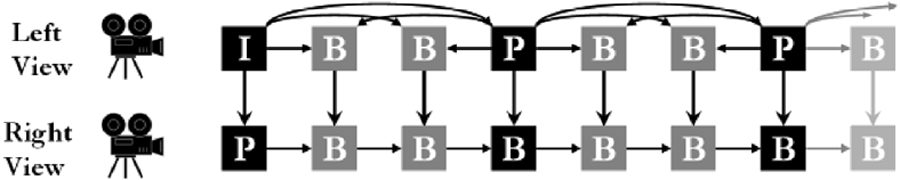
\includegraphics[width=0.8\textwidth]{predh262.png}
%\caption{Illustration of prediction in H.262/MPEG-2 Video multiview profile}
%\label{fig:predh262}
%\end{center}
%\end{figure}
%
%
%The combination of inter-view and temporal prediction is the basic principle for efficient compression of conventional stereo video. A corresponding standard specification has already been defined in ITU-T Rec. H.262/ISO/IEC 13818-2 MPEG-2 Video, the Multiview Profile \onlinecite{haskell1997digital, itu1994mpeg2}, as illustrated in Fig. \ref{fig:predh262}. The left eye view is encoded without reference to the right eye view, using standard MPEG-2. This ensures backward compatibility with Main Profile of H.262/MPEG-2 Video, since it is possible to decode the left eye view bit stream and to display 2-D video. For the right eye view, inter-view prediction is allowed in addition to temporal prediction.
%
%However, the gain in compression efficiency compared to independent encoding of both video streams is rather limited. This is mainly due to the fact that temporal prediction already provides very good performance. Typically, if temporal prediction is efficient for a certain image (e.g., B-pictures for right view in Fig. \ref{fig:predh262}) then additional inter-view prediction does not increase the coding performance significantly. Temporal neighbouring images are typically on average more similar than spatially neighbouring images.
%
%For images that are coded as I-pictures, i.e., without reference to other temporally adjacent images in the video sequence, a significant gain can be achieved by inter-view prediction. Typically every 0.5–1 s such I-pictures are inserted into a video stream to enable random access and error robustness. In Fig. \ref{fig:predh262}, the left-hand side picture of the left view is encoded as I-picture. The corresponding left-hand side picture of the right view would also be encoded as I-picture for random access when in- dependently encoding both video streams. However, in H.262/ MPEG-2 Video multiview coding, inter-view prediction can be applied, resulting in a significant increase of compression efficiency compared to coding this picture as I-picture.
%
%Research on compression of conventional stereo video has continued into several directions, including for instance optimum joined bit allocation for both channels, or abandoning backward compatibility to design more efficient inter-view prediction structures. Algorithms have been based on more up-to-date video codecs such as H.263\onlinecite{itu1995h263}, MPEG-4 Visual\onlinecite{itu1999mpeg4}, or H.264/AVC\onlinecite{sun2005stereo, wiegand2003overview, itu2003h264}. However, none of the developments including the original Multiview profile have reached commercial relevance so far, since the application of stereo video did not develop into a relevant mass market yet.
%
%\subsection{Compression of Video Plus Depth Data}
%
%An alternative to classical stereo video as described in the previous section is to transmit a video signal and a per sample depth map. From the video and depth information, a stereo pair can be rendered at the decoder \onlinecite{fehn2002evolutionary, fehn20043d}. This extends the functionality since it enables head motion parallax viewing if the user’s head motion is tracked. Additionally, this format is interesting from compression efficiency point of view. Per sample depth data can be regarded as a monochromatic, luminance-only video signal. The depth is restricted to a range between two extremes $Z_{near}$ and $Z_{far}$ indicating the minimum and maximum distance of the corresponding 3-D point from the camera respectively. The depth range is linearly quantized with 8 bit, i.e., the closest point is associated with the value 255 and the most distant point is associated with the value 0. With that, the depth map is specified, resulting in a grey scale image. These grey scale images can be fed into the luminance channel of a video signal and the chrominance can be set to a constant value. The resulting standard video signal can then be processed by any state-of-the-art video codec.
%
%Results from the European ATTEST project \onlinecite{fehn2002evolutionary} have shown that depth data can be very efficiently compressed this way. Several state-of-the-art video codecs have been tested (MPEG-2, MPEG-4, H.264/AVC). A course estimate indicates that 10\%–20\% of the bit rate which is necessary to encode the colour video is sufficient to encode the depth at good quality. This is due to the specific statistics of depth data, being on average smoother and less structured that colour data.
%
%Based on these observations, a new backward compatible (with respect to classical DVB) approach for 3DTV was developed in the ATTEST project. It uses a layered bit stream syntax. The base layer is a conventional 2-D colour video encoded using MPEG-2. This base layer can be processed by any existing MPEG-2 decoder providing backward compatibility. Additionally the bit stream contains an advanced layer carrying the encoded depth information. Advanced systems may access this layer to decode the depth stream and then generate a stereo pair to be displayed stereoscopically by view interpolation.
%
%This concept is highly interesting due to the backward compatibility, compression efficiency and extended functionality compared to conventional stereo video. Moreover, it does not introduce any specific coding algorithms. It is only necessary to specify high-level syntax that allows a decoder to interpret 2 incoming video streams correctly as colour and depth. Additionally information about depth range($Z_{near}$ and $Z_{far}$) needs to be transmitted. Therefore, MPEG specified a corresponding container format “ISO/IEC 23002-3 Representation of Auxiliary Video and Supplemental Information,” also known as MPEG-3 Part 3, for video plus depth data \onlinecite{iso2007rep, iso2007fdam}. Moreover, H.264/AVC contains an option to convey the depth images through its auxiliary picture syntax. Here, the video codec for the colour video signal and associated depth video signal are both H.264/AVC. This approach is backwards compatible with any existing deployment of H.264/AVC.
%
%A general problem of the video plus depth format is content creation, i.e., the generation of depth information. Cameras that automatically capture per pixel depth with the video are available and are being further enhanced, but the quality of the captured depth fields is currently still limited. Algorithms for depth estimation have been studied extensively in computer vision literature and powerful solutions are available. However, it always remains an estimation that can only be solved up to a residual error probability. Estimation errors influence the quality of rendered views. A fully automatic, accurate and reliable depth capturing system is still to be developed. User-assisted content generation is an option for specific applications. Even having perfect depth available, artifacts may occur in rendered views due to disocclusion. This effect increases with the distance of the virtual view from the original camera position. Additional occlusion layers (layered depth video as extension of layered depth images \onlinecite{shade1998layered}) or extension to multiview video plus depth \onlinecite{zitnick2004high, kauff2007depth}, help to minimize these problems at the cost of increased data rate and complexity.
%
%\subsection{Multiview Video Coding}
%
%\begin{figure}[htbp]
%\begin{center}
%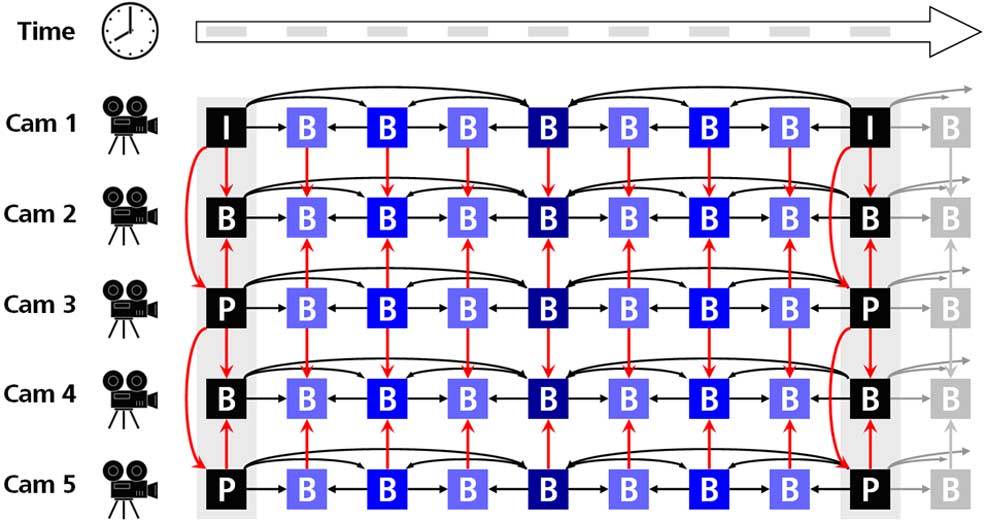
\includegraphics[width=0.8\textwidth]{tempinterpred.jpg}
%\caption{Temporal/inter-view prediction structure for MVC.}
%\label{fig:tempinterpred}
%\end{center}
%\end{figure}
%
%A common element of many 3DTV systems is the use of multiple views of the same scene that have to be transmitted to the user. The straight-forward solution for this would be to encode all video signals independently using a state-of-the-art video codec such as H.264/AVC. However, multiview video contains a large amount of inter-view statistical dependencies, since all cameras capture the same scene from different view-points. These can be exploited for combined temporal/inter-view prediction, as illustrated in Fig. \ref{fig:tempinterpred}. Images are not only predicted from temporally neighbouring images but also from corresponding images in adjacent views. Statistical evaluations have shown that significant gain can be expected from such combined temporal/inter-view prediction \onlinecite{merkle2005statistical, kaup2006analysis}. Pioneering work on multiview image coding is reported in \onlinecite{magnor2000data, magnor2003multi}.
%
%Several research groups addressed multiview video coding (MVC) and developed dedicated inter-view/temporal prediction structures to efficiently exploit all statistical dependencies within the multiview video data sets (see e.g., \onlinecite{oh12542multi, cheng2006multi, yang2006hyper, vetro2004coding, kalva2006design, socek2006permutation, kalva2006challenges, bilen2006multi}. Among those, algorithms that are based on hierarchical B-pictures \onlinecite{schwarz2006analysis} as supported by H.264/AVC syntax in temporal and inter-view dimension (Fig. \ref{fig:tempinterpred}) proved best performance in exhaustive experiments conducted in the context of MPEG standardization \onlinecite{flierl2007motion, merkle2006efficient, mueller2006multi, merkle2007efficient}. In these experiments, it has been shown by objective and subjective measurements that dedicated MVC outperforms independent encoding of the multiple video streams significantly. However, the achievable gain strongly depends on the content and its properties such as camera distance, frame rate and complexity of the content (motion, texture). For some data sets the peak signal-to-noise ratio (PSNR )gain was reported as 0.5 dB and below. Maximum reported gains were up to 3dB.
%
%A drawback of combined temporal/inter-view prediction as illustrated in Fig. \ref{fig:tempinterpred} is the complexity. This includes computational complexity, memory requirements and delay. In \onlinecite{merkle2007efficient, merkle2007coding}, it has been shown that the complexity can be significantly decreased without sacrificing much coding efficiency. Inter-view prediction is restricted here to the key pictures that would be treated as I-pictures in independent encoding of the views (e.g., time and in Fig. \ref{fig:tempinterpred}). Most of the coding gain of MVC comes from inter-view prediction of these pictures that do not use temporal prediction for temporal random access reasons. Omitting inter-view prediction for pictures that have a temporal reference does not cost much coding efficiency whereas it decreases complexity significantly.
%
%In addition to combined temporal/inter-view prediction, specific MVC algorithms have been proposed. The basic idea of depth/disparity-based view interpolation prediction \onlinecite{martinian2006view, kitahara2006multi, martinian2006extensions} is to estimate depth or disparity either at the encoder (this requires overhead for sending the depth/disparity) or the decoder, and to perform view interpolation or 3-D warping for prediction. However, the gains reported so far are marginal. Only for very few test data sets with very close camera settings such view interpolation prediction provides a gain of up to 5\% bit rate saving at the same visual quality. Further investigations are needed to optimize the performance.
%
%Further, illumination and color inconsistencies affect the exploitation of inter-view statistical dependencies. Usually such effects should be minimized by proper setting of the conditions, however, an MVC algorithm should also be able to cope with this as well, since proper white and color balancing of the input can not be guaranteed. Also, the illumination (spotlights, shadows, etc.) varies largely over the multiview images due to the lighting conditions. These problems might be handled by proper illumination and color compensation as proposed in \onlinecite{kim2006results} and \onlinecite{lee2006results}. The basic idea is to modify the motion compensation on macroblock level. Before subtracting the pixel values of the block to be encoded and the reference block, the mean of each is compensated from the corresponding pixel values. This assumes locally constant illumination and color variations, which is an appropriate model trading-off accuracy and complexity. Gains of up to 0.7 dB have been reported for some test data using illumination compensation. However, this strongly depends on the test data and in some cases the gain is negligible or there is none at all. On average over all test data sets a bit rate reduction of 5\% was reported for the same visual quality.
%
%An alternative to illumination compensation on macroblock level integrated into the encoding process, also an appropriate preprocessing can be applied, prior to encoding. Algorithms for illumination correction are well-known in image and video processing. Then the corrected data can be passed to a standard encoder. The big advantage of such an approach is that no changes are necessary to the encoder, decoder and bit stream syntax. A preliminary investigation in this direction is presented in \onlinecite{fecker2006improving}, however, results are not complete and performance in comparison to integrated illumination compensation is not clear.
%
%Another research direction is improving disparity estimation, compensation, and coding \onlinecite{lu2009effective}. Mostly disparity is treated equally to motion, however, it is known that the statistical properties of disparity vectors can be quite different compared to those of motion vectors. Disparity estimation has been studied extensively in the computer vision literature. Usually, basic geometric properties and constraints are taken into account. For instance, the search can be done along epipolar lines.
%
%This may lead to better estimates and reduce the complexity. Further, specific disparity coding may improve the efficiency of inter-view prediction. Specific coding modes for MVC such as the inter-view direct mode \onlinecite{guo2006inter} are under investigation.
%
%Combination of scalability with MVC is investigated for in- stance in \onlinecite{garbas20064d, drose2006extending, yang20064, yang2005scalable, ozbek2006scalable}. So far the feature of scalability only comes with decreased compression efficiency. Distributed MVC is investigated for instance in \onlinecite{guo2006distributed}. Also first work on efficient trans- port and delivery taking user interactivity into account has been presented \onlinecite{kurutepe-interactive, kurutepe2006interactive}. Finally, efficient mechanisms for optimum random access, parallel processing and memory management for MVC have been investigated.
%
%Since the results clearly indicate that MVC outperforms independent encoding of the multiple video signals, and there is a clear demand from industry for a corresponding standard, ISO/ MPEG and ITU/VCEG decided developing a dedicated MVC specification \onlinecite{vetro-joint, vetro2006joint}. It will be an extension of H.264/AVC (Amendment 4), which is scheduled to be finalized in 2008. MVC is the main focus of this Special Issue. We therefore refer the reader to the dedicated articles in this volume that contain all details of state-of-the-art MVC technology.
%
%\subsection{Conclusions and Future Research Directions}
%
%Research on coding of stereo video, multiview video and associated depth or disparity data has reached a good level of maturity. Related international standards are available enabling a variety of 3DTV systems and applications. However, compared to coding of other types of media data the scientific field is relatively young, and therefore there is still a lot of room for improvement of algorithms. This includes for instance optimization of MVC and development of new specific coding MVC algorithms. Depth or disparity coding may be improved further by development of dedicated algorithms. Further, there are more complex types of data representations for 3DTV such as layered depth video and multiview video plus depth that provide extended functionality. Efficient coding algorithms for such data are still under investigation. Initial results are reported in \onlinecite{merkle2007efficientmvc} and \onlinecite{merkle2007multi}. Other types of multiview representations are also under investigation often related to specific types of 3-D displays. An example is presented in \onlinecite{saishu2006flatbed}.
%
%%\cleardoublepage

\chapter{外文资料的书面翻译}

\section{摘要}

最近,3D电视技术相关的研究工作在全球范围内都有增加。这些研究覆盖了整个媒体处理流程,从采集到显示无所不包。不同的3D电视系统依靠各种类型数据构成的不同的3D场景表示方式。对这些数据的高效编码对于3D电视的成功至关重要。对双目视频、多视点视频、深度图或视差图中像素类型数据的压缩拓展了已有的经典视频编码的原则。针对多视点视频和视频加深度数据的强大算法和开放的国际标准已经出现并一直有着进展,这为在不久的将来引进各种3D电视系统奠定了基础。对3D网格模型的压缩也达到了高度成熟的程度。对静态的几何体,有多种强大的算法可以有效地压缩顶点和连接数据量。对动态3D几何体的压缩是现在更受关注的研究方向。基于时间的预测是一个重要的对动画3D网格序列去冗余信息的机制。容错性对于在易出错的信道上传输数据十分重要,而多描述编码(MDC)是一种可行的保护数据的方法。对静态图和2D视频的MDC已经得到了广泛的研究,但是对多视点视频和3D网格的MDC最近才刚刚提出。用水印进行3D数据的知识产权保护也是一个前沿的研究方向。3D水印方法方面的文献根据表示场景的主要部分在应用算法前后的维数可以归为三类。总而言之,3D电视编码技术正在走向成熟。相关系统和服务可能在不久的将来进入市场。然而,这个方向的研究相对其他媒体数据的研究而言又很少,所以仍有很大的空间可以改进,有很多新的算法可能被提出。

\section{简介}

将我们的视觉延伸到三维空间在近几十年中一直都在研究,但是大规模的消费市场仍然没有发展起来。3D视频还在小众市场发展,包括专业应用(比如科学数据可视化、医药学等)和娱乐方面(比如IMAX影院、3D游戏等)。近年来,更多的研究精力投向了这个领域,以期能够跨越阻碍3D视频应用得到更广泛成功应用的障碍\cite{smolic20063d, onural2004overview, smolic20043dav, smolic2005interactive, onural2006assessment}。从获得信号、处理信号到3D场景表示、编码、传输,再到渲染和3D显示,整个处理流水线的各个部分都取得了显著的进步。很可能在不久的将来,各种3D视频系统、组件、应用和服务就会进入市场。

这一期中给出了各种尖端3D视频技术的综述,分别针对一个3D视频处理流水线中的一个特定组件。这篇文章介绍编码相关的部分。\onlinecite{alatan2007scene}中介绍了用在不同的3D视频系统和应用中的不同3D场景表示格式在。这些格式整合了各种类型的数据,比如多视点视频、深度或3D网格的几何数据。总的来说,3D视频就意味着有大量的数据需要传输、存储和水印。于是高效的压缩就是3D视频成功与否的一个关键条件。同时对发明一个鲁棒的3D水印技术来保护所有权也有很强的需求。此外,开放的国际标准对市场和相关商业的发展也是一个推动力。ISO/IEC JTC1/SC29/WG11 (Moving Picture Experts Group—MPEG)就是一个在数字媒体标准化中起到重要作用的国际标准化组织。所以,这篇文章关注现有的和正在成形的各种数据的MPEG标准。

接下来的几节分别给出多视点视频、深度和关联数据的编码综述,集中关注已有的和正在成形的MPEG标准。第3节介绍用于3D视频表示以及3D计算机图形学的静态和动态3D网格数据的压缩。容错以及3D视频的多描述编码(MDC)在第4节中介绍。然后在第5节中介绍用水印保护3D内容的方法。最后,第6节概况和总结这篇文章的观点。

\section{多视点视频、深度和关联数据编码}

很多3D电视系统都基于场景,这些3D场景由N个相机获取(见\onlinecite{tanimoto2004free, fujii2002free, matsuyama2004real, hamaguchi2003real, carranza2003free, wurmlin20033d, wurmlin20043d, matusik20043d})。最简单的情形就是经典的两路视频构成的立体视频,更复杂一些的系统用8路、16路或更多路相机获取的视频。有些系统还使用可以当作视频信号的深度信息。这一节综述这类数据的压缩算法和标准。更早对这个研究方向的综述可以参见\onlinecite{shum2003survey}。通过共享内容、共享一些相机,多视点视频比起单视点视频的编码可以一定提升。在多视点视频编码中,除了挖掘单个相机的数据在时间上的关联之外,临近的相机之间的关系也被挖掘出来。于是多视点视频在单视点视频的基础上增加了一个新的压缩维度:视点间的方向。

\subsection{传统立体视频编码}

立体视频是多视点视频中最重要的一个特例,是有N=2个视点的情形。 压缩传统的立体视频已经经过了长时间的研究,相关的标准也已经问世。一个传统的立体对由从两个略微不同的视点(对应人的瞳距)观察同一场景的两幅静态图组成。这两幅图片总的来说极其相似,使得它们很适合压缩,比如从一幅图片预测另一幅。例如,其中一幅可以不参考另一幅而单独压缩,而第二幅图片可以从已经编码的一幅图片来预测,就像视频压缩中的基于时间预测的动态补偿那样。
 
对两幅图片的样本基于场景和相机属性(包括位置和相机内部参数比如焦距)的3D几何各自对应起来。每个样本的位移或视差就等价于一个视频序列中两幅连续图像的dense motion field。于是就可以用运动估计和运动补偿一样的方法去做视差分析和视差补偿,以此实现图像预测,然后就只需要编码预测误差或者进一步的残差即可。

然而,一些特定的动态补偿和视差补偿间的区别需要考虑进来。视差向量场的统计与运动向量场的统计不同。视差是有偏的,而且相对较大。零视差以为着一个点在 3D场景中的深度极大,而一个距离相近很近的3D点会有很大的视差值。这需要对视差向量的熵编码做调整。总的来说,在正常的帧率下,视频序列中在时间上邻近的图像倾向于比立体视频的两个视点的图像更加相似。图像损失(内容在一张图中可见但是在另一张图中不存在,也就无法被预测)平均来说在立体视频中出现得比时间上邻近的两幅图更多。此外,立体图片对中的差别可能来自不正确的白平衡或色彩平衡,也可能来自场景的光照和表面反射效果的差别。 

\begin{figure}[htbp]
\begin{center}
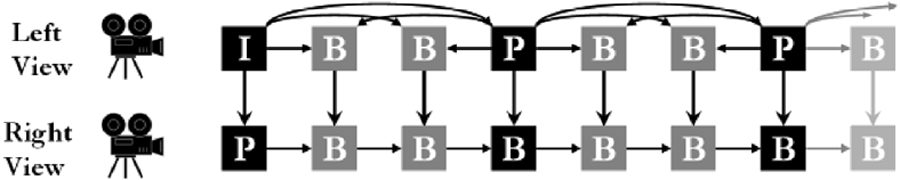
\includegraphics[width=0.8\textwidth]{predh262.png}
\caption{H.262/MPEG-2视频多视点类(multiview profile)的预测示意}
\label{fig:predh262chs}
\end{center}
\end{figure}

视角间和时间上的预测组合是有效压缩传统立体视频的基本方法。对应的标准已经在ITU-T Rec.H.262/ISO/IEC 13818-2 MPEG-2Video, the Multiview Profile\cite{haskell1997digital, itu1994mpeg2}中定义了,如图\ref{fig:predh262chs}所示。左眼视频不参考右眼视频单独编码,使用标准的MPEG-2。这保证了对H.262/MPEG-2的主类(Main Profile)的前向兼容性,因为这样可以解码左眼视频流来显示2D视频。对右眼视频,时间轴预测之外还可以允许做视点间预测。
 
然而,对比分别压缩两个视频流而言,这样的压缩效率提升很有限。这主要是由于基于时间的预测已经达到了很高的性能。特别是当基于时间的预测对于一张特定图像效率不错的时候(比如图\ref{fig:predh262chs}中右眼视频的B帧),那么增加视角间的预测就无法显著提升编码性能了。时间上邻近的图像平均而言一般都比空间上邻近的图像更相似。

对于编码为I帧的图像,也就是说不参考其他视频序列中时间上邻近的帧来编码的帧,加入视角间的预测有明显成效。一般每半秒到一秒时间就会在视频序列中插入这样一个I帧来保证随机访问和容错性。在图\ref{fig:predh262chs}中,左眼序列的最左侧一帧被编码为I帧,当分别编码两个视频序列时,对应的右眼序列中的那一帧也可以编码为I帧。但是在H.262/MPEG-2视频多视点编码中,可以采用视角间预测来达到压缩效率上比编为I帧方式的显著提升。

对于传统立体视频压缩的研究还在各个方向上继续进行着,包括对各个频道的最优码率分配以及放弃前向兼容去设计一个更加有效的视角间预测的结构。相关算法是都是基于更新的视频编码比如H.263\cite{itu1995h263},MPEG-4 Visual\cite{itu1999mpeg4}或H.264/AVC \cite{sun2005stereo, wiegand2003overview, itu2003h264}。但是由于立体视频的应用还没有发展到一个足够大的市场,所有这些进展包括原有的多视点类(Multiview profile)都尚未能商业化。

\subsection{视频加深度数据的压缩}

除了前文描述的经典立体视频外,还有一种传输视频信号的方式——传输一路视频和每个样本的深度图。从视频和深度信息,可以在解码端渲染出一对立体图\cite{fehn2002evolutionary,fehn20043d}。这提供了另一项功能:当用户的头部移动被捕捉到时,能够提供相对应的观察角度的图像。此外,这种格式从压缩效率的角度来看很有价值。深度信息可以被当作单色、仅有明度的视频信号。深度被限制在两个表示对应3D点到摄像机的最小和最大距离的极限距离$Z_{near}$和$Z_{far}$之间。深度范围线性地量子化到8位,也就是最近的点赋值255,最远点赋值为0。这样一来,一张深度图就确定下来了,成为一张灰度图。这些灰阶图可以被插入视频信号的光照信道中,其色彩可以被设定为一个常数。这样获得的标准视频信号就可以用任何先进的视频编码处理了。

欧洲ATTEST的一个项目\cite{fehn2002evolutionary}结果表明深度信息可以用这种方式非常高效地压缩。一些前沿的视频编码参与了测试(MPEG-2, MPEG-4, H.264/AVC)。一项估计显示,只要编码彩色视频信号10\%到20\%的比特率就足以编码高质量的深度信息了。

基于这些观察,这个ATTEST项目提出了一种新的(对比经典的DVB)向前兼容的实现3DTV的方式。它采用一种分层的比特流语法。基层是一个传统的 MPEG-2编码的彩色2D视频。基层可以被任何现有的MPEG-2解码器处理,保证前向兼容性。除此之外,比特流还包含更高一层传输编码后的深度信息。更高级的系统可以访问这一层来解码深度信息,然后通过插值生成一对立体图像来显示。

这种概念由于保证了前向兼容性、压缩率高并且相比传统立体视频功能扩展更多,所以非常有价值。不仅如此,它并不引入一种特定的编码算法。只需要制定一种高层的语法,让解码器能够把输入的两路视频正确地分辨成一路视频和一路深度即可。附加的深度信息($Z_{near}$和$Z_{far}$)需要另外传输。所以MPEG为视频加深度信息制定了一种对应的容器格式 “ISO/IEC 23002-3 Representation of Auxiliary Video and Supplemental Information”,或者称为MPEG-3 Part 3\cite{iso2007rep, iso2007fdam}。此外,H.264/AVC包含一个选项通过辅助的图片语法传输深度图。此处对彩色视频信号和对应的深度视频信号的视频编码都用的是 H.264/AVC。这种方法对任何已部署的H.264/AVC设备都能做到前向兼容。

对视频加深度的格式而言,有一个普遍存在的问题就是深度信息的生成。能够在捕获视频的同时自动获取每个像素深度的摄像机已经问世而且在进一步增强,但是得到的深度场的精度还是很有限。计算机视觉相关的文献中对深度估计的算法有了很深入的研究,强大的解决方案也已经出现。但是这总是一个建立在一定残差误差概率上的估计值。估计的误差会影响渲染出的图像的质量。全自动而且精确的深度获取系统仍然有待开发。对于特定的应用,用户辅助的内容生成可以作为一种选择。即使有了完美的深度图,遮挡也会使渲染出的图像有瑕疵。这些效应在距离原始摄像机位更远的虚拟点上会更加严重。增加一些层(深度视频层作为深度图像层的扩展\cite{shade1998layered})或者扩展到多视点视频加深度\cite{zitnick2004high, kauff2007depth}能够以增加数据量和复杂度为代价,帮助减小这些问题。

\subsection{多视点视频编码}

\begin{figure}[htbp]
\begin{center}
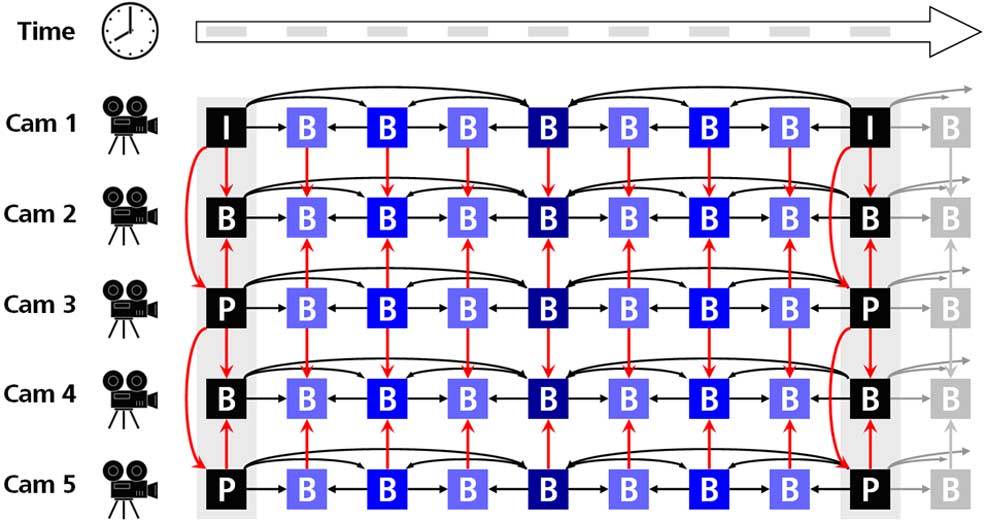
\includegraphics[width=0.8\textwidth]{tempinterpred.jpg}
\caption{MVC的时间和视角间预测结构}
\label{fig:tempinterpredchs}
\end{center}
\end{figure}

3DTV系统的一个共同部分是传输给用户的同一场景不同视角视频的使用。最直接的解决方法就是把所有的视频信号分别用最新的编码方式比如 H.264/AVC编码。但是多视点视频在视角间存在统计意义上很大的相关性,因为每个摄像机捕获的都是不同视角的同一场景的图像。这些相关性可以用来进行时间和视角间预测,如图\ref{fig:tempinterpredchs}所示。图像不仅仅根据时间上临近的图来预测,还根据相邻视角的对应图像预测。统计表明这样的组合式预测能够极大地提高编码效率\cite{merkle2005statistical, kaup2006analysis}。多视点图像编码的前沿研究在\onlinecite{magnor2000data, magnor2003multi}中有报告。

几个研究小组提出了多视点视频(MVC),并且发展了专门的视角间和时间预测的架构来有效地挖掘利用多视点视频数据集中的统计相关性(见\onlinecite{oh12542multi, cheng2006multi, yang2006hyper, vetro2004coding, kalva2006design, socek2006permutation, kalva2006challenges, bilen2006multi})。其中,H.264/AVC时间和视角间预测的语法支持的基于B帧的算法\cite{schwarz2006analysis}在MPEG标准的穷尽测试下被证明是性能最好的\cite{flierl2007motion, merkle2006efficient, mueller2006multi, merkle2007efficient}。在这些实验中,客观和主观的测量都显示MVC极大地超越了独立压缩各个视频。然而,能够获得的提升极其依赖内容和相机间距、帧率、内容复杂度(运动、纹理)等属性。对于一些数据集,信噪比峰值(PSNR)增益在0.5dB以下。最大的增益达到过3dB。

图\ref{fig:tempinterpredchs}中描述的时间和视角间组合预测的一个不足就是其复杂度。包括计算复杂度、内存需求和延迟。在\onlinecite{merkle2007efficient, merkle2007coding}中提到,复杂度在不牺牲多少编码效率的情形下可以极大地降低。视角间预测此时被限制在作为I帧独立编码的关键帧上(例如图\ref{fig:tempinterpredchs}中的$t_0$和$t_8$)。MVC中大部分编码增益来自于这些为了随机访问而不进行视角间预测的帧。忽略有时间预测的帧的视角间预测并不消耗多少编码效率却显著降低复杂度。

在结合时间和视角间预测之外,专门的MVC算法被提了出来。基于深度/视差的视角间插值预测\cite{martinian2006view, kitahara2006multi, martinian2006extensions}的基本思想是在编码(这需要另外传输深度/视差)或解码端估计深度或视差,然后进行视角间插值或者3D扭曲来预测。但是目前得到的增益不高。仅仅对于摄像机参数极其接近的很小一部分数据集,这样的视角间插值预测在同样画质下能节省5\%的比特率。想要优化性能还要做进一步的研究。

不仅如此,光照和色彩的不一致影响了对视角间统计相关性的挖掘。通常这样的效应能被正确的条件设定减小,但是 MVC算法也要能够应对这样的情形,因为输入的白平衡和色彩平衡并不能保证。同样,一定的光照条件下,光照(聚光灯、阴影等)在视角间会有很大的不同。这些问题或许能通过\onlinecite{kim2006results}和\onlinecite{lee2006results}中提出的正确的光照和色彩补偿来解决。基本思想是在宏块级别修改运动补偿。在对待编码帧块和参考块的像素值相减之前,二者的平均值根据对应的像素值做补偿。其中假设了本地的光照和色彩变化是常值,这是个模型的准确率和复杂度之间的权衡。对于一些测试数据,光照补偿获得了0.7dB的增益。但是这个增益极大地依靠测试数据,在一些情况下,增益可以忽略甚至根本不存在。对所有的测试数据集平均下来,相同视觉质量下,能够节省5\%的比特率。

另一种宏块级别的光照补偿可以整合到编码过程中,一个合适的预处理也可以在编码前进行。对图像和视频的光照更正算法广为人知。然后更正过的数据可以被传到一个标准的编码器。这种方法的一大优势是编码器、解码器和码流语法不需要做任何改动。一项这个方向上的前期调研发表在\onlinecite{fecker2006improving}中,但是结果并不完全,性能与整合光照补偿的比较也不清楚。

另一个研究方向是改进视差估计、补偿和编码\cite{lu2009effective}。多数的视差都被当作运动来对待,但是我们知道视差向量的统计属性和运动向量可以完全不同。视差估计在计算机视觉文献中已经被广泛研究。通常,级别的几何属性和约束会考虑进来。比如搜索可以通过沿着核极线(epipolar lines)完成。这可能带来更好的估计和降低复杂度。此外,专门的视差编码或许能提高视角间预测的编码效率。专门的MVC编码模式比如视角间直接模式\cite{guo2006inter}正在研究中。

MVC的扩展性结合正在被研究,比如\onlinecite{garbas20064d, drose2006extending, yang20064, yang2005scalable, ozbek2006scalable}。目前可扩展的功能仅能依靠降低压缩效率。分布式MVC在\onlinecite{guo2006distributed}中被研究。加入用户交互考虑的有效传输在\onlinecite{kurutepe-interactive, kurutepe2006interactive}中初次被讨论。最后,能够随机访问的有效的MVC编码机制、并行处理和内存管理也正在研究中。

由于结果明显表明MVC优于单独编码各路视频信号,业界又显然需要一个对应的标准,ISO/MPEG和ITU/VCEG 决定发展一种专门的MVC标准\cite{vetro-joint, vetro2006joint}。这会是一个H.264/AVC的扩展(第4修正案),这预计在2008年内完工。MVC是这一期特刊的主要关注点。我们因此向读者介绍包含最前沿MVC技术的文章。

\subsection{结论和未来研究方向}

对立体视频、多视点视频和相关深度、视差数据的研究已经有很高的成熟度。相关的国际标准也已经问世,使3DTV系统和应用成为可能。然而,相对于其他类型和媒体数据的编码,这个领域还很年轻,算法还有很大的进步空间。这包括对MVC实力的优化和新的专门的MVC算法的开发。深度和视差编码可能在将来的专门的算法中进一步优化。此外,有更多复杂的3DTV数据结构比如分层的深度视频和多视点视频加深度来提供更多的功能。对这些数据的有效编码算法还在研究之中。初步的结果在\onlinecite{merkle2007efficientmvc}和\onlinecite{merkle2007multi}中有报告。其他多视点描述的类型也在研究中,这往往和特定的一类3D显示器相关。\onlinecite{saishu2006flatbed}中有一个例子。

\begin{center}
\heiti{原文索引}
\end{center}

Smolic A, M{\"u}eller K, Stefanoski N, et al. Coding algorithms for 3DTV—a survey. IEEE transactions on circuits and systems for video technology, 2007, 17(11):1606–1620

%\cleardoublepage
%  
%%% Local Variables: 
%%% mode: latex
%%% TeX-master: t
%%% End: 

\chapter{实验数据表格}
\label{cha:expdatatable}

\begin{longtable}[\textwidth]{lrrr}
\caption{VS2008性能分析报告(前50项记录)}\label{tab:vs50}\\
\toprule[1.5pt]
\multicolumn{1}{l}{\textbf{Function Name}} & \multicolumn{1}{r}{\textbf{Exclusive Time}} & \multicolumn{1}{r}{\textbf{Exclusive Time \%}} & \multicolumn{1}{r}{\textbf{Number of Calls}}\\
\midrule[1.5pt]
\endfirsthead
\multicolumn{4}{c}{续表~\thetable\hskip1em VS2008性能分析报告(前50项记录)}\\
\toprule[1.5pt]
\multicolumn{1}{l}{\textbf{Function Name}} & \multicolumn{1}{r}{\textbf{Exclusive Time}} & \multicolumn{1}{r}{\textbf{Exclusive Time \%}} & \multicolumn{1}{r}{\textbf{Number of Calls}}\\ 
\midrule[1pt]
\endhead
\hline
\multicolumn{4}{r}{续下页}
\endfoot
\endlastfoot
\rowcolor{gray!15}
    macroblockPredGetDataUV		&	341.01	&	14.41	&	2,632,478	\\
    macroblockPredGetDataY		&	321.37	&	13.58	&	1,316,239	\\ \rowcolor{gray!15}
    idct4x4\_c						&	316.86	&	13.39	&	5,028,960	\\
    macroblockGetPred\_axb		&	181.29	&	7.66 	&	1,316,239	\\ \rowcolor{gray!15}
    macroblockGetPred\_axb\_Bi	&	133.42	&	5.64 	&	571,944		\\
    macroblockGetHalfPel			&	132.47	&	5.6  	&	148,552		\\ \rowcolor{gray!15}
    Filter							&	101.92	&	4.31 	&	6,215,308	\\
    addMacroblockdata				&	85.36	&	3.61 	&	184,171		\\ \rowcolor{gray!15}
    iquant4x4\_c					&	84.48	&	3.57 	&	5,028,960	\\
    macroblockPBPrediction		&	70.95	&	3    	&	184,171		\\ \rowcolor{gray!15}
    macroblockInterDecode\_uv		&	67.05	&	2.83 	&	184,171		\\
    save\_data\_pb					&	55.32	&	2.34 	&	200,880		\\ \rowcolor{gray!15}
    macroblockInterDecode16x16\_y	&	54.34	&	2.3  	&	184,171		\\
    PSliceDecode					&	46.38	&	1.96 	&	124			\\ \rowcolor{gray!15}
    macroblock\_read\_cavlc\_B\_slice	
    								&	37.29	&	1.58 	&	155,520		\\
    GetHorFilterStrength			&	33.17	&	1.4  	&	3,325,760	\\ \rowcolor{gray!15}
    CheckMvDataB					&	31.38	&	1.33 	&	4,916,240	\\
    getRefXYDirectB				&	29.65	&	1.25 	&	582,670		\\ \rowcolor{gray!15}
    macroblockIntraDecode\_y		&	26.87	&	1.14 	&	26,429		\\
    FilterMB						&	25.12	&	1.06 	&	210,600		\\ \rowcolor{gray!15}
    calc\_B\_skip\_refs			&	19.16	&	0.81 	&	145,645		\\
    LumaHorFilter					&	14.34	&	0.61 	&	210,600		\\ \rowcolor{gray!15}
    macroblockIntraDecode\_uv		&	14.24	&	0.6  	&	26,429		\\
    setRefXY						&	13.78	&	0.58 	&	2,330,348	\\ \rowcolor{gray!15}
    LumaVerFilter					&	13.15	&	0.56 	&	210,600		\\
    unscan\_zig\_4x4				&	12.03	&	0.51 	&	2,942,655	\\ \rowcolor{gray!15}
    GetVerFilterStrength			&	9.82 	&	0.42 	&	3,325,760	\\
    macroblock\_read\_cavlc\_P\_slice	
    								&	8.92 	&	0.38 	&	45,360		\\ \rowcolor{gray!15}
    ChromaHorFilter				&	8.86 	&	0.37 	&	210,600		\\
    ChromaVerFilter				&	8.7  	&	0.37 	&	210,600		\\ \rowcolor{gray!15}
    require\_data\_decode			&	7.72 	&	0.33 	&	184,171		\\
    macroblock\_processor\_PB		&	6.02 	&	0.25 	&	4,464		\\ \rowcolor{gray!15}
    iquant2x2dc\_c					&	4.67 	&	0.2  	&	421,200		\\
    idct8x8							&	4.66 	&	0.2  	&	21,920		\\ \rowcolor{gray!15}
    T264dec\_mb\_read\_intra\_cavlc
    								&	3.61 	&	0.15 	&	26,429		\\
    CheckMvDataP					&	2.55 	&	0.11 	&	868,249		\\ \rowcolor{gray!15}
    block\_residual\_read\_cavlc	&	2.52 	&	0.11 	&	106,045		\\
    ISliceDecode					&	2.47 	&	0.1  	&	6			\\ \rowcolor{gray!15}
    save\_data						&	2.46 	&	0.1  	&	9,720		\\
    iquant8x8\_c					&	2.31 	&	0.1  	&	21,920		\\ \rowcolor{gray!15}
    process\_data\_decode\_I		&	2.31 	&	0.1  	&	26,429		\\
    macroblock\_read\_cavlc\_PB\_y
    								&	2.26 	&	0.1  	&	15,493		\\ \rowcolor{gray!15}
    do\_16x16\_luma\_prediction	&	2.24 	&	0.09 	&	21,359		\\
    idct4x4dc\_c					&	2.01 	&	0.08 	&	21,359		\\ \rowcolor{gray!15}
    \_printf						&	1.89 	&	0.08 	&	911			\\
    do\_8x8\_luma\_prediction		&	1.85 	&	0.08 	&	15,560		\\ \rowcolor{gray!15}
    require\_data\_decode\_I		&	1.6  	&	0.07 	&	26,429		\\
    macroblock\_read\_cavlc\_uv	&	1.31 	&	0.06 	&	41,922		\\ \rowcolor{gray!15}
    do\_8x8\_chroma\_prediction	&	1.29 	&	0.05 	&	52,858		\\
    BitstreamGetBits				&	1.21 	&	0.05 	&	580,391		\\
    \bottomrule[1.5pt]
\end{longtable}

\begin{longtable}[\textwidth]{lrrr}
\caption{VTune性能分析报告(前50项记录)}\label{tab:vtune50}\\
\toprule[1.5pt]
\multicolumn{1}{l}{\textbf{Function}} & \multicolumn{1}{r}{\textbf{Calls}} & \multicolumn{1}{r}{\textbf{Self Time}} & \multicolumn{1}{r}{\textbf{\% in fuction}}\\
\midrule[1.5pt]
\endfirsthead
\multicolumn{4}{c}{续表~\thetable\hskip1em VTune性能分析报告(前50项记录)}\\
\toprule[1.5pt]
\multicolumn{1}{l}{\textbf{Function}} & \multicolumn{1}{r}{\textbf{Calls}} & \multicolumn{1}{r}{\textbf{Self Time}} & \multicolumn{1}{r}{\textbf{\% in fuction}}\\ 
\midrule[1pt]
\endhead
\hline
\multicolumn{4}{r}{续下页}
\endfoot
\endlastfoot
	\rowcolor{gray!15}
    macroblockPredGetDataUV	&	2632478	&	774863	&	0.61	\\
    macroblockPredGetDataY	&	1316239	&	702575	&	0.58	\\ \rowcolor{gray!15}
    idct4x4\_c					&	5028960	&	398076	&	1		\\
    macroblockInterDecode16x16\_y	
    							&	184171	&	328834	&	0.46	\\ \rowcolor{gray!15}
    macroblockGetPred\_axb	&	1316239	&	311730	&	0.11	\\
    FilterMB					&	210600	&	203506	&	0.21	\\ \rowcolor{gray!15}
    Filter						&	6215308	&	191937	&	1		\\
    iquant4x4\_c				&	5028960	&	157459	&	1		\\ \rowcolor{gray!15}
    macroblockInterDecode\_uv	&	184171	&	154697	&	0.48	\\
    macroblockPBPrediction	&	184171	&	150609	&	0.05	\\ \rowcolor{gray!15}
    macroblockGetHalfPel		&	148552	&	134793	&	1		\\
    macroblockGetPred\_axb\_Bi&	571944	&	132951	&	0.05	\\ \rowcolor{gray!15}
    GetVerFilterStrength		&	3325760	&	125372	&	0.64	\\
    GetHorFilterStrength		&	3325760	&	117207	&	0.65	\\ \rowcolor{gray!15}
    CheckMvDataB				&	4916240	&	115925	&	1		\\
    calc\_B\_skip\_refs		&	145645	&	83987	&	0.47	\\ \rowcolor{gray!15}
    addMacroblockdata			&	184171	&	82547	&	1		\\
    save\_data\_pb				&	200880	&	66356	&	0.76	\\ \rowcolor{gray!15}
    setRefXY					&	2330348	&	59615	&	1		\\
    LumaHorFilter				&	210600	&	56700	&	0.49	\\ \rowcolor{gray!15}
    LumaVerFilter				&	210600	&	56175	&	0.46	\\
    unscan\_zig\_4x4			&	2942655	&	55896	&	1		\\ \rowcolor{gray!15}
    macroblock\_read\_cavlc\_B\_slice
    							&	155520	&	55255	&	0.23	\\
    macroblockIntraDecode\_y	&	26429	&	47460	&	0.42	\\ \rowcolor{gray!15}
    ChromaVerFilter			&	210600	&	37978	&	0.51	\\
    ChromaHorFilter			&	210600	&	37163	&	0.55	\\ \rowcolor{gray!15}
    getRefXYDirectB			&	582670	&	36556	&	1		\\
    macroblock\_processor\_PB	&	4464 	&	29068	&	0.01	\\ \rowcolor{gray!15}
    macroblockIntraDecode\_uv	&	26429	&	28597	&	0.5		\\
    PSliceDecode				&	124  	&	19439	&	0		\\ \rowcolor{gray!15}
    CheckMvDataP				&	868249	&	18065	&	1		\\
    macroblock\_read\_cavlc\_P\_slice	
    							&	45360	&	13979	&	0.36	\\ \rowcolor{gray!15}
    \_security\_check\_cookie	&	942387	&	13589	&	1		\\
    block\_residual\_read\_cavlc	
    							&	106045	&	12540	&	0.64	\\ \rowcolor{gray!15}
    iquant2x2dc\_c				&	421200	&	9292 	&	1		\\
    T264dec\_mb\_read\_intra\_cavlc	
    							&	26429	&	9065 	&	0.31	\\ \rowcolor{gray!15}
    require\_data\_decode		&	184171	&	8725 	&	1		\\
    BitstreamGetBits			&	580391	&	8431 	&	1		\\ \rowcolor{gray!15}
    idct8x8						&	21920	&	4918 	&	1		\\
    macroblock\_read\_cavlc\_PB\_y	
    							&	15493	&	3735 	&	0.42	\\ \rowcolor{gray!15}
    process\_data\_decode\_I	&	26429	&	3681 	&	0.02	\\
    save\_data					&	9720 	&	3592 	&	1		\\ \rowcolor{gray!15}
    ProcessData				&	1    	&	2619 	&	0		\\
    idct4x4dc\_c				&	21359	&	2584 	&	1		\\ \rowcolor{gray!15}
    iquant8x8\_c				&	21920	&	2566 	&	1		\\
    macroblock\_read\_cavlc\_uv	
    							&	41922	&	2561 	&	0.55	\\ \rowcolor{gray!15}
    require\_data\_decode\_I	&	26429	&	2389 	&	1		\\
    do\_16x16\_luma\_prediction	
    							&	21359	&	2251 	&	0.96	\\ \rowcolor{gray!15}
    do\_8x8\_luma\_prediction	&	15560	&	2192 	&	0.93	\\
    T264dec\_mb\_read\_coff\_token\_t0	
    							&	83162	&	2112 	&	1		\\
    \bottomrule[1.5pt]
\end{longtable}

\begin{longtable}[\textwidth]{lrrrr}
\caption{不同视频解码速度一览(基准性能)}\label{tab:desktopBaseline}\\
\toprule[1.5pt]
\multicolumn{1}{l}{\textbf{Clip Name}} & \multicolumn{1}{r}{\textbf{Threads(s)}} & \multicolumn{1}{r}{\textbf{Time(ms)}} & \multicolumn{1}{r}{\textbf{Decoding FPS}} & \multicolumn{1}{r}{\textbf{Viewer FPS}}\\
\midrule[1.5pt]
\endfirsthead
\multicolumn{5}{c}{续表~\thetable\hskip1em 不同视频解码速度一览(基准性能)}\\
\toprule[1.5pt]
\multicolumn{1}{l}{\textbf{Clip Name}} & \multicolumn{1}{r}{\textbf{Decoding Threads(s)}} & \multicolumn{1}{r}{\textbf{Decoding Time(ms)}} & \multicolumn{1}{r}{\textbf{Decoding FPS}} & \multicolumn{1}{r}{\textbf{Viewer FPS}}\\
\midrule[1pt]
\endhead
\hline
\multicolumn{5}{r}{续下页}
\endfoot
\endlastfoot
\rowcolor{gray!15}
dual144		&	1	&	249		&	522.34	&	261.17	\\
dual288		&	1	&	877		&	148.25	&	74.12	\\ \rowcolor{gray!15}
dual576		&	1	&	3855	&	33.72	&	16.86	\\
dual720		&	1	&	8754	&	14.85	&	7.43	\\ \rowcolor{gray!15}
golf25		&	1	&	827		&	241.80	&	30.23	\\
golf25dual	&	1	&	199		&	251.13	&	125.56	\\ \rowcolor{gray!15}
golf623		&	1	&	26344	&	189.19	&	23.65	\\
race81		&	1	&	3773	&	171.73	&	21.47	\\ \rowcolor{gray!15}
single144	&	1	&	115		&	563.08	&	563.08	\\
single288	&	1	&	363		&	178.94	&	178.94	\\ \rowcolor{gray!15}
single576	&	1	&	1489	&	43.65	&	43.65	\\
single720	&	1	&	3343	&	19.44	&	19.44	\\ \rowcolor{gray!15}
\bottomrule[1.5pt]
\end{longtable}

\begin{longtable}[\textwidth]{lrrrr}
\caption{不同视频解码速度一览(MS编译器)}\label{tab:desktopMS}\\
\toprule[1.5pt]
\multicolumn{1}{l}{\textbf{Clip Name}} & \multicolumn{1}{r}{\textbf{Threads(s)}} & \multicolumn{1}{r}{\textbf{Time(ms)}} & \multicolumn{1}{r}{\textbf{Decoding FPS}} & \multicolumn{1}{r}{\textbf{Viewer FPS}}\\
\midrule[1.5pt]
\endfirsthead
\multicolumn{5}{c}{续表~\thetable\hskip1em 不同视频解码速度一览(MS编译器)}\\
\toprule[1.5pt]
\multicolumn{1}{l}{\textbf{Clip Name}} & \multicolumn{1}{r}{\textbf{Decoding Threads(s)}} & \multicolumn{1}{r}{\textbf{Decoding Time(ms)}} & \multicolumn{1}{r}{\textbf{Decoding FPS}} & \multicolumn{1}{r}{\textbf{Viewer FPS}}\\
%\midrule[1pt]
\endhead
%\hline
\multicolumn{5}{r}{续下页}
\endfoot
\endlastfoot
dual144 & 1 & 219 & 593.61 & 296.80\\ \hline
dual288 & 1 & 813 & 159.90 & 79.95\\ \hline
dual576 & 1 & 3422 & 37.99 & 18.99\\ \hline
dual720 & 1 & 7765 & 16.74 & 8.37\\ \hline
golf25 & 1 & 765 & 261.44 & 32.68\\ \hline
golf25dual & 1 & 187 & 267.38 & 133.69\\ \hline
golf623 & 1 & 23328 & 213.65 & 26.71\\ \hline
race81 & 1 & 3328 & 194.71 & 24.34\\ \hline
single144 & 1 & 93 & 698.92 & 698.92\\ \hline
single288 & 1 & 328 & 198.17 & 198.17\\ \hline
single576 & 1 & 1344 & 48.36 & 48.36\\ \hline
single720 & 1 & 3047 & 21.33 & 21.33\\ \hline
dual144 & 2 & 125 & 1040.00 & 520.00\\ \hline
dual288 & 2 & 407 & 319.41 & 159.71\\ \hline
dual576 & 2 & 2063 & 63.02 & 31.51\\ \hline
dual720 & 2 & 4843 & 26.84 & 13.42\\ \hline
golf25 & 2 & 391 & 511.51 & 63.94\\ \hline
golf25dual & 2 & 94 & 531.91 & 265.96\\ \hline
golf623 & 2 & 12969 & 384.30 & 48.04\\ \hline
race81 & 2 & 1687 & 384.11 & 48.01\\ \hline
single144 & 2 & 62 & 1048.39 & 1048.39\\ \hline
single288 & 2 & 187 & 347.59 & 347.59\\ \hline
single576 & 2 & 719 & 90.40 & 90.40\\ \hline
single720 & 2 & 2125 & 30.59 & 30.59\\ \hline
dual144 & 3 & 94 & 1382.98 & 691.49\\ \hline
dual288 & 3 & 297 & 437.71 & 218.86\\ \hline
dual576 & 3 & 1625 & 80.00 & 40.00\\ \hline
dual720 & 3 & 4094 & 31.75 & 15.88\\ \hline
golf25 & 3 & 266 & 751.88 & 93.98\\ \hline
golf25dual & 3 & 78 & 641.03 & 320.51\\ \hline
golf623 & 3 & 10297 & 484.02 & 60.50\\ \hline
race81 & 3 & 1218 & 532.02 & 66.50\\ \hline
single144 & 3 & 63 & 1031.75 & 1031.75\\ \hline
single288 & 3 & 187 & 347.59 & 347.59\\ \hline
single576 & 3 & 766 & 84.86 & 84.86\\ \hline
single720 & 3 & 2203 & 29.51 & 29.51\\ \hline
dual144 & 4 & 78 & 1666.67 & 833.33\\ \hline
dual288 & 4 & 250 & 520.00 & 260.00\\ \hline
dual576 & 4 & 1891 & 68.75 & 34.37\\ \hline
dual720 & 4 & 4656 & 27.92 & 13.96\\ \hline
golf25 & 4 & 219 & 913.24 & 114.16\\ \hline
golf25dual & 4 & 62 & 806.45 & 403.23\\ \hline
golf623 & 4 & 10093 & 493.81 & 61.73\\ \hline
race81 & 4 & 1079 & 600.56 & 75.07\\ \hline
single144 & 4 & 62 & 1048.39 & 1048.39\\ \hline
single288 & 4 & 171 & 380.12 & 380.12\\ \hline
single576 & 4 & 609 & 106.73 & 106.73\\ \hline
single720 & 4 & 1719 & 37.81 & 37.81\\
\bottomrule[1.5pt]
\end{longtable}

\begin{longtable}[\textwidth]{lrrrr}
\caption{不同视频解码速度一览(ICC编译器)}\label{tab:desktopICC}\\
\toprule[1.5pt]
\multicolumn{1}{l}{\textbf{Clip Name}} & \multicolumn{1}{r}{\textbf{Threads(s)}} & \multicolumn{1}{r}{\textbf{Time(ms)}} & \multicolumn{1}{r}{\textbf{Decoding FPS}} & \multicolumn{1}{r}{\textbf{Viewer FPS}}\\
\midrule[1.5pt]
\endfirsthead
\multicolumn{5}{c}{续表~\thetable\hskip1em 不同视频解码速度一览(ICC编译器)}\\
\toprule[1.5pt]
\multicolumn{1}{l}{\textbf{Clip Name}} & \multicolumn{1}{r}{\textbf{Decoding Threads(s)}} & \multicolumn{1}{r}{\textbf{Decoding Time(ms)}} & \multicolumn{1}{r}{\textbf{Decoding FPS}} & \multicolumn{1}{r}{\textbf{Viewer FPS}}\\
%\midrule[1pt]
\endhead
%\hline
\multicolumn{5}{r}{续下页}
\endfoot
\endlastfoot
dual144 & 1 & 219 & 593.61 & 296.80\\ \hline
dual288 & 1 & 813 & 159.90 & 79.95\\ \hline
dual576 & 1 & 3422 & 37.99 & 18.99\\ \hline
dual720 & 1 & 7765 & 16.74 & 8.37\\ \hline
golf25 & 1 & 765 & 261.44 & 32.68\\ \hline
golf25dual & 1 & 187 & 267.38 & 133.69\\ \hline
golf623 & 1 & 23328 & 213.65 & 26.71\\ \hline
race81 & 1 & 3328 & 194.71 & 24.34\\ \hline
single144 & 1 & 93 & 698.92 & 698.92\\ \hline
single288 & 1 & 328 & 198.17 & 198.17\\ \hline
single576 & 1 & 1344 & 48.36 & 48.36\\ \hline
single720 & 1 & 3047 & 21.33 & 21.33\\ \hline
dual144 & 2 & 125 & 1040.00 & 520.00\\ \hline
dual288 & 2 & 407 & 319.41 & 159.71\\ \hline
dual576 & 2 & 2063 & 63.02 & 31.51\\ \hline
dual720 & 2 & 4843 & 26.84 & 13.42\\ \hline
golf25 & 2 & 391 & 511.51 & 63.94\\ \hline
golf25dual & 2 & 94 & 531.91 & 265.96\\ \hline
golf623 & 2 & 12969 & 384.30 & 48.04\\ \hline
race81 & 2 & 1687 & 384.11 & 48.01\\ \hline
single144 & 2 & 62 & 1048.39 & 1048.39\\ \hline
single288 & 2 & 187 & 347.59 & 347.59\\ \hline
single576 & 2 & 719 & 90.40 & 90.40\\ \hline
single720 & 2 & 2125 & 30.59 & 30.59\\ \hline
dual144 & 3 & 94 & 1382.98 & 691.49\\ \hline
dual288 & 3 & 297 & 437.71 & 218.86\\ \hline
dual576 & 3 & 1625 & 80.00 & 40.00\\ \hline
dual720 & 3 & 4094 & 31.75 & 15.88\\ \hline
golf25 & 3 & 266 & 751.88 & 93.98\\ \hline
golf25dual & 3 & 78 & 641.03 & 320.51\\ \hline
golf623 & 3 & 10297 & 484.02 & 60.50\\ \hline
race81 & 3 & 1218 & 532.02 & 66.50\\ \hline
single144 & 3 & 63 & 1031.75 & 1031.75\\ \hline
single288 & 3 & 187 & 347.59 & 347.59\\ \hline
single576 & 3 & 766 & 84.86 & 84.86\\ \hline
single720 & 3 & 2203 & 29.51 & 29.51\\ \hline
dual144 & 4 & 78 & 1666.67 & 833.33\\ \hline
dual288 & 4 & 250 & 520.00 & 260.00\\ \hline
dual576 & 4 & 1891 & 68.75 & 34.37\\ \hline
dual720 & 4 & 4656 & 27.92 & 13.96\\ \hline
golf25 & 4 & 219 & 913.24 & 114.16\\ \hline
golf25dual & 4 & 62 & 806.45 & 403.23\\ \hline
golf623 & 4 & 10093 & 493.81 & 61.73\\ \hline
race81 & 4 & 1079 & 600.56 & 75.07\\ \hline
single144 & 4 & 62 & 1048.39 & 1048.39\\ \hline
single288 & 4 & 171 & 380.12 & 380.12\\ \hline
single576 & 4 & 609 & 106.73 & 106.73\\ \hline
single720 & 4 & 1719 & 37.81 & 37.81\\
\bottomrule[1.5pt]
\end{longtable}

% \end{appendix}
% \end{example}
%
% \myentry{致谢声明}
% \DescribeEnv{ack}
% 把致谢做成一个环境更好一些,直接往里面写感谢的话就可以啦!下面是数学系一位同
% 学致谢里的话,拿过来做个广告,多希望每个人都能写这么一句啊!
% \begin{example}
% \begin{ack}
%   ……
%   还要特别感谢计算机系薛瑞尼同学在论文格式和 \LaTeX{} 编译等方面给我的很多帮助!
% \end{ack}
% \end{example}
%
% \myentry{列表环境}
% \DescribeEnv{itemize}
% \DescribeEnv{enumerate}
% \DescribeEnv{description}
% 为了适合中文习惯,模板将这三个常用的列表环境用 \pkg{paralist} 对应的压缩环境替
% 换。一方面满足了多余空间的清楚,另一方面可以自己指定标签的样式和符号。细节请参
% 看 \pkg{paralist} 文档,此处不再赘述。
%
% \changes{v3.0}{2007/05/12}{没有了综合论文训练页面,很多本科论文专用命令就消失了。}
%
% \subsection{数学环境}
% \label{sec:math}
% \thuthesis{} 定义了常用的数学环境:
%
% \begin{center}
% \begin{tabular}{*{7}{l}}\hline
%   axiom & theorem & definition & proposition & lemma & conjecture &\\
%   公理 & 定理 & 定义 & 命题 & 引理 & 猜想 &\\\hline
%   proof & corollary & example & exercise & assumption & remark & problem \\
%   证明 & 推论 & 例子& 练习 & 假设 & 注释 & 问题\\\hline
% \end{tabular}
% \end{center}
%
% 比如:
% \begin{example}
% \begin{definition}
% 道千乘之国,敬事而信,节用而爱人,使民以时。
% \end{definition}
% \end{example}
% 产生(自动编号):\\[5pt]
% \fbox{{\hei 定义~1.1~~~} {道千乘之国,敬事而信,节用而爱人,使民以时。}}
%
% 列举出来的数学环境毕竟是有限的,如果想用{\hei 胡说}这样的数学环境,那么很容易定义:
% \begin{example}
% \newtheorem{nonsense}{胡说}[chapter]
% \end{example}
%
% 然后这样使用:
% \begin{example}
% \begin{nonsense}
% 契丹武士要来中原夺武林秘笈。\pozhehao 慕容博
% \end{nonsense}
% \end{example}
% 产生(自动编号):\\[5pt]
% \fbox{{\hei 胡说~1.1~~~} {契丹武士要来中原夺武林秘笈。\kern0.3ex\rule[0.8ex]{2em}{0.1ex}\kern0.3ex 慕容博}}
%
% \subsection{自定义以及其它}
% \label{sec:othercmd}
% 模板的配置文件 thuthesis.cfg 中定义了很多固定词汇,一般无须修改。如果有特殊需求,
% 推荐在导言区使用 \cs{renewcommand}。当然,导言区里可以直接使用中文。
%
%
%\section{致谢}
%\label{sec:thanks}
%
% 在模板的开发和维护过程中,我得到不少同学的热情支持,如:edyfox@newsmth 编写
% 了 Makefile,Truel@newsmth 编写了 msmake.cmd,oseen@newsmth 将其移植到 UTF-8 并
% 制作了 Debian package,特别感谢 MagicGlaive@newsmth 为 2008 年本科论文格式修改
% 作出的一切!
%
% 感谢我自己能把这件事坚持下来,模板制作期间颇多感慨,不断遇到问题,不断摸索解决。其中的
% 酸甜苦辣恐怕只有自己能体会得到!
%
% 感谢所有在论文致谢中提及 \thuthesis{} 或者本人的同学:每当这个时候我都有说不出
% 的欣慰。大家的认可才是 \thuthesis{} 最大的动力。与此同时我也感觉到更大的压力,
% 因为模板的维护需要花费相当的精力。同时我对模板还不太满意,代码质量不高,结构组
% 织不好,文档内容不足。我呼唤感兴趣的同学能出手相助,给模板的开发和维护注入新的
% 活力,让我们一起把 \thuthesis{} 做得更好!
%
% \StopEventually{\PrintChanges\PrintIndex}
% \clearpage
%
% \section{实现细节}
%
% \subsection{基本信息}
%    \begin{macrocode}
%<cls>\NeedsTeXFormat{LaTeX2e}[1999/12/01]
%<cls>\ProvidesClass{thuthesis}
%<cfg>\ProvidesFile{thuthesis.cfg}
%<cls|cfg>[2008/02/28 4.5.1 Tsinghua University Thesis Template]
%    \end{macrocode}
%
% \subsection{定义选项}
% \label{sec:defoption}
% TODO: 所有的选项用 \pkg{xkeyval} 来重构,现在的太罗唆了。
%
% 定义文档所使用编码
%    \begin{macrocode}
%<*cls>
\newif\ifthu@UTF
\newif\ifthu@GBK
\DeclareOption{utf}{\thu@UTFtrue\thu@GBKfalse}
\DeclareOption{gbk}{\thu@GBKtrue\thu@UTFfalse}
%    \end{macrocode}
%
% 定义论文类型以及是否涉密
% \changes{v2.4}{2006/04/14}{添加模板名称命令。}
% \changes{v2.5}{2006/05/19}{增加本科论文的提交选项 submit。}
% \changes{v2.5.1}{2006/05/24}{如果没有设置格式选项,报错。}
% \changes{v2.5.1}{2006/05/26}{submit 只能由本科用。}
% \changes{v2.5.3}{2006/06/03}{submit 选项的一个笔误。}
% \changes{v3.0}{2007/05/12}{删除 submit 选项。}
%    \begin{macrocode}
\hyphenation{Thu-Thesis}
\def\thuthesis{\textsc{ThuThesis}}
\def\version{4.5}
\newif\ifthu@bachelor\thu@bachelorfalse
\newif\ifthu@master\thu@masterfalse
\newif\ifthu@doctor\thu@doctorfalse
\newif\ifthu@secret\thu@secretfalse
\DeclareOption{bachelor}{\thu@bachelortrue}
\DeclareOption{master}{\thu@mastertrue}
\DeclareOption{doctor}{\thu@doctortrue}
\DeclareOption{secret}{\thu@secrettrue}
%    \end{macrocode}
%
% 使用 dvips,dvipdfm, pdflatex 还是 xelatex
% \changes{v2.5.1}{2006/05/24}{如果选项设置了 dvips,但是用 pdflatex 编译,报错。}
% \changes{v2.6}{2006/06/09}{增加 dvipdfm 选项。}
% \changes{v4.5}{2009/01/03}{增加 xetex, pdftex 选项。}
%    \begin{macrocode}
\newif\ifthu@dvips
\newif\ifthu@dvipdfm
\newif\ifthu@xetex
\newif\ifthu@pdftex
\DeclareOption{dvips}{\thu@dvipstrue}
\DeclareOption{dvipdfm}{\thu@dvipdfmtrue}
\DeclareOption{pdftex}{\thu@pdftextrue}
\DeclareOption{xetex}{\thu@xetextrue}
%    \end{macrocode}
%
% 如果需要使用 arial 字体,请打开 [arial] 选项
%    \begin{macrocode}
\newif\ifthu@arial
\DeclareOption{arial}{\thu@arialtrue}
%    \end{macrocode}
%
% 目录中英文是否用 arial
%    \begin{macrocode}
\newif\ifthu@arialtoc
\DeclareOption{arialtoc}{\thu@arialtoctrue}
%    \end{macrocode}
% 章节标题中的英文是否用 arial
%    \begin{macrocode}
\newif\ifthu@arialtitle
\DeclareOption{arialtitle}{\thu@arialtitletrue}
%    \end{macrocode}
%
% 将选项传递给 book 类
%    \begin{macrocode}
\DeclareOption*{\PassOptionsToClass{\CurrentOption}{book}}
%    \end{macrocode}
%
% \cs{ExecuteOptions} 的参数之间用逗号分割,不能有空格。开始不知道,折腾了老半
% 天。
% \changes{v2.5.1}{2006/05/24}{ft,研究生院目录要 times,而教务处要 arial。}
% \changes{v2.5.1}{2006/05/26}{本科 openright,研究生 openany。}
% \changes{v3.1}{2007/10/09}{本科的目录又不要 arial 字体了。}
%    \begin{macrocode}
\ExecuteOptions{utf,arialtitle}
\ProcessOptions\relax
\LoadClass[12pt,a4paper,openany]{book}
%    \end{macrocode}
%
% 用户至少要提供一个选项:指定论文类型。
%    \begin{macrocode}
\ifthu@bachelor\relax\else
  \ifthu@master\relax\else
    \ifthu@doctor\relax\else
      \ClassError{thuthesis}%
                 {You have to specify one of thesis options: bachelor, master or doctor.}{}
    \fi
  \fi
\fi      
%    \end{macrocode}
%
% 检查用户指定的选项和实际编译命令是否冲突。
%    \begin{macrocode}
\RequirePackage{ifpdf,ifxetex}
\ifthu@xetex\RequireXeTeX\fi
\def\RequirePDFTeX{%
  \ifpdf\else
    \ClassError{thuthesis}%
               {pdflatex is required to compile this document!}{}
  \fi}
\ifthu@pdftex\RequirePDFTeX\fi
\def\thu@checkoption#1#2{%
  \@for\reserved@a:=#2\do{%
    \csname ifthu@\reserved@a\endcsname
      \ClassError{thuthesis}%
                 {Please remove `\reserved@a' option when you run #1.}{}
    \fi}}
\ifpdf\thu@checkoption{pdflatex}{dvips,dvipdfm,xetex}\thu@pdftextrue\fi % force the option to be true
\ifxetex\thu@checkoption{xelatex}{dvips,dvipdfm,pdftex}\thu@xetextrue\fi
%    \end{macrocode}
%
%
% \subsection{装载宏包}
% \label{sec:loadpackage}
%
% 引用的宏包和相应的定义。
%    \begin{macrocode}
\RequirePackage{ifthen,calc}
%    \end{macrocode}
%
% \AmSTeX{} 宏包,用来排出更加漂亮的公式。
%    \begin{macrocode}
\RequirePackage{amsmath,amssymb}
%    \end{macrocode}
%
% 用很爽的 \pkg{txfonts} 替换 \pkg{mathptmx} 宏包,同时用它自带的 typewriter 字
% 体替换 courier。必须出现在 \AmSTeX{} 之后。
% \changes{v3.1}{2007/06/16}{replace mathptmx with txfonts.}
%    \begin{macrocode}
\RequirePackage{txfonts}
%    \end{macrocode}
%
% 图形支持宏包。
%    \begin{macrocode}
\RequirePackage{graphicx}
%    \end{macrocode}
%
% 并排图形。\pkg{subfigure} 已经不再推荐,用新的 \pkg{subfig}。加入 |config| 选项
% 以便兼容 \pkg{subfigure} 的命令。浮动图形和表格标题样式。\pkg{caption2} 已经不
% 推荐使用,采用新的 \pkg{caption}。它会自动被 \pkg{subfig} 装载进来。所以可以在
% 后面看到 \cs{captionsetup} 的命令。
%    \begin{macrocode}
\RequirePackage[config]{subfig}
%    \end{macrocode}
%
% 首行缩进宏包
%    \begin{macrocode}
\RequirePackage{indentfirst}
%    \end{macrocode}
%
% 更好的列表环境。
% \changes{v2.6.2}{2006/06/18}{去掉 \pkg{paralist} 的 newitem 和 newenum 选项,因为默
% 认是打开的。}
% \changes{v2.6.4}{2006/10/23}{增加 \texttt{neverdecrease} 选项。}
%    \begin{macrocode}
\RequirePackage[neverdecrease]{paralist}
%    \end{macrocode}
%
% 中文支持宏包。XeTeX 模式下直接调用 \pkg{xeCJK},一切问题都搞定了。
% \changes{v4.5}{2008/01/03}{加入 XeTeX 支持,需要 \pkg{xeCJK}。}
%    \begin{macrocode}
\ifthu@xetex
  \RequirePackage{mathptmx} % fontspec conflicts with txfonts now, so we have to load other times-math fonts.
  \RequirePackage{xunicode,xltxtra}
  \RequirePackage[CJKnumber,CJKtextspaces,CJKmathspaces]{xeCJK}
  %\punctstyle{kaiming}
  \punctstyle{quanjiao}
  % todo: minor fix of CJKnumb
  \def\CJK@null{\kern\CJKnullspace\Unicode{48}{7}\kern\CJKnullspace}
  \defaultfontfeatures{Mapping=tex-text} % after fontspec
%    \end{macrocode}
% 默认采用 Adobe 的四款 (宋,黑,楷,仿宋) 免费字体。这样的话,缺少隶书和幼圆。本
% 科的封面大字会受影响。请手动替换。
%    \begin{macrocode}
  \setCJKmainfont[BoldFont={Adobe Heiti Std}, ItalicFont={Adobe Kaiti Std}]{Adobe Song Std}
  \setCJKsansfont{Adobe Heiti Std}
  \setCJKmonofont{Adobe Kaiti Std}
  \setCJKfamilyfont{song}{Adobe Song Std}
  \setCJKfamilyfont{hei}{Adobe Heiti Std}
  \setCJKfamilyfont{fs}{Adobe Fangsong Std}
  \setCJKfamilyfont{kai}{Adobe Kaiti Std}
  \setCJKfamilyfont{li}{LiSu} % todo: 用隶书字体代替
  \setCJKfamilyfont{you}{YouYuan} % todo: 用幼圆字体代替
  %\setCJKfamilyfont{li}{CTLiShuSJ} % todo: 用隶书字体代替
  %\setCJKfamilyfont{you}{CTZhongYuanSJ} % todo: 用幼圆字体代替

  \setmainfont{Times New Roman}
  \setsansfont{Arial}
  \setmonofont{Courier New} 
%    \end{macrocode}
% 对于 \LaTeX\ 和 PDF\LaTeX,调用 \pkg{CJK} 以及相关的包。注意:\pkg{CJKpunct} 必
% 须放在 \pkg{CJKspace} 之前。
%    \begin{macrocode}
\else
  \RequirePackage{CJKutf8}
  \RequirePackage{CJKnumb}
  \ifthu@GBK % CJKpunct 在 UTF 下工作的不好。
    \IfFileExists{CJKpunct.sty}%
                 {\RequirePackage{CJKpunct}}%
                 {\ClassWarning{thuthesis}{no CJKpunct.sty availiable!}}
  \fi
  \RequirePackage{CJKspace}
%    \end{macrocode}
% arial 字体需要单独安装,如果不使用 arial 字体,可以用 helvet 字体 |\textsf|
% 模拟,二者基本没有差别。
%    \begin{macrocode}
  \ifthu@arial
    \IfFileExists{arial.sty}%
                 {\RequirePackage{arial}}%
                 {\ClassWarning{thuthesis}{no arial.sty availiable!}}
  \fi
\fi
%    \end{macrocode}
%
% 可拷贝的 PDF (\pkg{ccmap} 结合 \texttt{pdflatex} 和 \texttt{dvipdfmx} 使用)
%    \begin{macrocode}
\ifthu@dvips\else
  \ifthu@xetex\else
    \RequirePackage{ccmap}
  \fi
\fi
%    \end{macrocode}
%
% 定理类环境宏包,其中 \pkg{amsmath} 选项用来兼容 \AmSTeX{} 的宏包
%    \begin{macrocode}
\RequirePackage[amsmath,thmmarks,hyperref]{ntheorem}
%    \end{macrocode}
%
% 表格控制
% \changes{v2.6}{2006/06/09}{增加 \pkg{longtable}。}
%    \begin{macrocode}
\RequirePackage{array}
\RequirePackage{longtable}
%    \end{macrocode}
%
% 使用三线表:\cs{toprule},\cs{midrule},\cs{bottomrule}。
%    \begin{macrocode}
\RequirePackage{booktabs}
%    \end{macrocode}
%
% 参考文献引用宏包。
%    \begin{macrocode}
\RequirePackage[numbers,super,sort&compress]{natbib}
%    \end{macrocode}
%
% 生成有书签的 pdf 及其开关,请结合 gbk2uni 避免书签乱码。
% \changes{v2.6}{2006/06/09}{去除 hyperref 选项,等待全局传递。}
%    \begin{macrocode}
\RequirePackage{hyperref}
\ifxetex
  \hypersetup{%
    CJKbookmarks=true}
\else
  \hypersetup{%
    unicode=true,
    CJKbookmarks=false}
\fi
\hypersetup{%
  bookmarksnumbered=true,
  bookmarksopen=true,
  bookmarksopenlevel=1,
  breaklinks=true,
  colorlinks=false,
  plainpages=false,
  pdfpagelabels,
  pdfborder=0 0 0}
%    \end{macrocode}
%
% dvips 模式下网址断字有问题,加入这个包解决之。
% \changes{v4.4}{2008/05/12}{修复网址断字。}
%    \begin{macrocode}
\ifthu@dvips
  \RequirePackage{breakurl}
\fi
%    \end{macrocode}
%
% 设置 url 样式,与上下文一致
%    \begin{macrocode}
\urlstyle{same}
%    \end{macrocode}
%
% \pkg{hypernat} 让 \pkg{hyperref} 和 \pkg{natbib} 协调的工作。应该
% 在 \pkg{natbib} 和 \pkg{hyperref} 之后加载,参看其文档。
%    \begin{macrocode}
\RequirePackage{hypernat}
%</cls>
%    \end{macrocode}
%
%
% \subsection{主文档格式}
% \label{sec:mainbody}
%
% \subsubsection{Three matters}
% 我们的单面和双面模式与常规的不太一样。
% \changes{v2.5.1}{2006/05/23}{本科正文之后页码即用罗马数字,研究生不变。}
% \changes{v2.5.3}{2006/06/03}{第一章永远右开。}
% \changes{v4.4}{2008/05/30}{本科正文后的页码延续前面的阿拉伯数字,不再用罗马数
% 字。}
% \changes{v4.4}{2008/05/30}{本科取消了所有页眉,毫无疑问,在以后的修订中还会加
% 上的,我们等着看。}
%    \begin{macrocode}
%<*cls>
\renewcommand\frontmatter{%
  \if@openright\cleardoublepage\else\clearpage\fi
  \@mainmatterfalse
  \pagenumbering{Roman}
  \pagestyle{thu@empty}}
\renewcommand\mainmatter{%
  \if@openright\cleardoublepage\else\clearpage\fi
  \@mainmattertrue
  \pagenumbering{arabic}
  \ifthu@bachelor\pagestyle{thu@plain}\else\pagestyle{thu@headings}\fi}
\renewcommand\backmatter{%
  \if@openright\cleardoublepage\else\clearpage\fi
  \@mainmattertrue}
%</cls>
%    \end{macrocode}
%
%
% \subsubsection{字体}
% \label{sec:font}
%
% \begin{macro}{\song}
% \begin{macro}{\songti}
% \begin{macro}{\fs}
% \begin{macro}{\fangsong}
% \begin{macro}{\kai}
% \begin{macro}{\kaishu}
% \begin{macro}{\hei}
% \begin{macro}{\heiti}
% \begin{macro}{\li}
% \begin{macro}{\lishu}
% \begin{macro}{\you}
% \begin{macro}{\youyuan}
% 重定义字体命令
%    \begin{macrocode}
%<*cls>
\newcommand{\song}{\CJKfamily{song}}    % 宋体
\def\songti{\song}
\newcommand{\fs}{\CJKfamily{fs}}        % 仿宋体
\def\fangsong{\fs}
\newcommand{\kai}{\CJKfamily{kai}}      % 楷体
\def\kaishu{\kai}
\newcommand{\hei}{\CJKfamily{hei}}      % 黑体
\def\heiti{\hei}
\newcommand{\li}{\CJKfamily{li}}        % 隶书
\def\lishu{\li}
\newcommand{\you}{\CJKfamily{you}}      % 幼圆
\def\youyuan{\you}
%    \end{macrocode}
% \end{macro}
% \end{macro}
% \end{macro}
% \end{macro}
% \end{macro}
% \end{macro}
% \end{macro}
% \end{macro}
% \end{macro}
% \end{macro}
% \end{macro}
% \end{macro}
%
% 重定义字号命令
%
% Ref 1:
% \begin{verbatim}
% 参考科学出版社编写的《著译编辑手册》(1994年)
% 七号       5.25pt       1.845mm
% 六号       7.875pt      2.768mm
% 小五       9pt          3.163mm
% 五号      10.5pt        3.69mm
% 小四      12pt          4.2175mm
% 四号      13.75pt       4.83mm
% 三号      15.75pt       5.53mm
% 二号      21pt          7.38mm
% 一号      27.5pt        9.48mm
% 小初      36pt         12.65mm
% 初号      42pt         14.76mm
%
% 这里的 pt 对应的是 1/72.27 inch,也就是 TeX 中的标准 pt
% \end{verbatim}
%
% Ref 2:
% WORD 中的字号对应该关系如下:
% \begin{verbatim}
% 初号 = 42bp = 14.82mm = 42.1575pt
% 小初 = 36bp = 12.70mm = 36.135 pt
% 一号 = 26bp = 9.17mm = 26.0975pt
% 小一 = 24bp = 8.47mm = 24.09pt
% 二号 = 22bp = 7.76mm = 22.0825pt
% 小二 = 18bp = 6.35mm = 18.0675pt
% 三号 = 16bp = 5.64mm = 16.06pt
% 小三 = 15bp = 5.29mm = 15.05625pt
% 四号 = 14bp = 4.94mm = 14.0525pt
% 小四 = 12bp = 4.23mm = 12.045pt
% 五号 = 10.5bp = 3.70mm = 10.59375pt
% 小五 = 9bp = 3.18mm = 9.03375pt
% 六号 = 7.5bp = 2.56mm
% 小六 = 6.5bp = 2.29mm
% 七号 = 5.5bp = 1.94mm
% 八号 = 5bp = 1.76mm
%
% 1bp = 72.27/72 pt
% \end{verbatim}
%
% \begin{macro}{\thu@define@fontsize}
% \changes{v2.6.2}{2006/06/18}{引入此命令重新定义字号。}
% 根据习惯定义字号。用法:
%
% \cs{thu@define@fontsize}\marg{字号名称}\marg{磅数}
%
% 避免了字号选择和行距的紧耦合。所有字号定义时为单倍行距,并提供选项指定行距倍数。
%    \begin{macrocode}
\newlength\thu@linespace
\newcommand{\thu@choosefont}[2]{%
   \setlength{\thu@linespace}{#2*\real{#1}}%
   \fontsize{#2}{\thu@linespace}\selectfont}
\def\thu@define@fontsize#1#2{%
  \expandafter\newcommand\csname #1\endcsname[1][\baselinestretch]{%
    \thu@choosefont{##1}{#2}}}
%    \end{macrocode}
% \end{macro}
% \begin{macro}{\chuhao}
% \begin{macro}{\xiaochu}
% \begin{macro}{\yihao}
% \begin{macro}{\xiaoyi}
% \begin{macro}{\erhao}
% \begin{macro}{\xiaoer}
% \begin{macro}{\sanhao}
% \begin{macro}{\xiaosan}
% \begin{macro}{\sihao}
% \begin{macro}{\banxiaosi}
% \begin{macro}{\xiaosi}
% \begin{macro}{\dawu}
% \begin{macro}{\wuhao}
% \begin{macro}{\xiaowu}
% \begin{macro}{\liuhao}
% \begin{macro}{\xiaoliu}
% \begin{macro}{\qihao}
% \begin{macro}{\bahao}
%    \begin{macrocode}
\thu@define@fontsize{chuhao}{42bp}
\thu@define@fontsize{xiaochu}{36bp}
\thu@define@fontsize{yihao}{26bp}
\thu@define@fontsize{xiaoyi}{24bp}
\thu@define@fontsize{erhao}{22bp}
\thu@define@fontsize{xiaoer}{18bp}
\thu@define@fontsize{sanhao}{16bp}
\thu@define@fontsize{xiaosan}{15bp}
\thu@define@fontsize{sihao}{14bp}
\thu@define@fontsize{banxiaosi}{13bp}
\thu@define@fontsize{xiaosi}{12bp}
\thu@define@fontsize{dawu}{11bp}
\thu@define@fontsize{wuhao}{10.5bp}
\thu@define@fontsize{xiaowu}{9bp}
\thu@define@fontsize{liuhao}{7.5bp}
\thu@define@fontsize{xiaoliu}{6.5bp}
\thu@define@fontsize{qihao}{5.5bp}
\thu@define@fontsize{bahao}{5bp}
%    \end{macrocode}
% \end{macro}
% \end{macro}
% \end{macro}
% \end{macro}
% \end{macro}
% \end{macro}
% \end{macro}
% \end{macro}
% \end{macro}
% \end{macro}
% \end{macro}
% \end{macro}
% \end{macro}
% \end{macro}
% \end{macro}
% \end{macro}
% \end{macro}
% \end{macro}
%
% 正文小四号 (12pt) 字,行距为固定值 20 磅。
%    \begin{macrocode}
\renewcommand\normalsize{%
  \@setfontsize\normalsize{12bp}{20bp}
  \abovedisplayskip=10bp \@plus 2bp \@minus 2bp
  \abovedisplayshortskip=10bp \@plus 2bp \@minus 2bp
  \belowdisplayskip=\abovedisplayskip
  \belowdisplayshortskip=\abovedisplayshortskip}
%</cls>
%    \end{macrocode}
%
%
% \subsubsection{页面设置}
% \label{sec:layout}
% 本来这部分应该是最容易设置的,但根据格式规定出来的结果跟学校的 WORD 样例相差很
% 大,所以只能微调。
% \changes{v2.4}{2006/04/14}{把页面尺寸写入 dvi,避免有的用户通
%   过 dvips 不指定页面类型而得到古怪的结果。}
%    \begin{macrocode}
%<*cls>
\AtBeginDvi{\special{papersize=\the\paperwidth,\the\paperheight}}
\AtBeginDvi{\special{!%
      \@percentchar\@percentchar BeginPaperSize: a4
      ^^Ja4^^J\@percentchar\@percentchar EndPaperSize}}
\setlength{\textwidth}{\paperwidth}
\setlength{\textheight}{\paperheight}
\setlength\marginparwidth{0cm}
\setlength\marginparsep{0cm}
\addtolength{\textwidth}{-6.4cm}
\setlength{\oddsidemargin}{3.2cm-1in}
\setlength{\evensidemargin}{\oddsidemargin}
\setlength{\headheight}{20pt}
\setlength{\topskip}{0pt}
\setlength{\skip\footins}{15pt}
\setlength{\topmargin}{2.8cm-1in}
\ifthu@bachelor
  \setlength{\footskip}{1.3cm}
  \setlength{\headsep}{0.6cm}
  \addtolength{\textheight}{-7.8cm}
\else
  \setlength{\footskip}{1.5cm}
  \setlength{\headsep}{0.5cm}
  \addtolength{\textheight}{-8.6cm}
\fi
%</cls>
%    \end{macrocode}
%
% \subsubsection{页眉页脚}
% \label{sec:headerfooter}
% 新的一章最好从奇数页开始 (openright),所以必须保证它前面那页如果没有内容也必须
% 没有页眉页脚。(code stolen from \pkg{fancyhdr})
%    \begin{macrocode}
%<*cls>
\let\thu@cleardoublepage\cleardoublepage
\newcommand{\thu@clearemptydoublepage}{%
  \clearpage{\pagestyle{empty}\thu@cleardoublepage}}
\let\cleardoublepage\thu@clearemptydoublepage
%    \end{macrocode}
%
% 定义页眉和页脚。chapter 自动调用 thispagestyle{thu@plain},所以要重新定义 thu@plain。
% \changes{v2.0}{2005/12/18}{以前的太乱了,重新整理过清晰多了。}
% \changes{v2.1}{2006/03/01}{彻底放弃 fancyhdr,定义自己的样式。}
% \changes{v2.5}{2006/05/13}{本科的奇偶页眉不同。}
% \changes{v2.5}{2006/05/20}{增加 empty 页面样式。}
% \begin{macro}{\ps@thu@empty}
% \begin{macro}{\ps@thu@plain}
% \begin{macro}{\ps@thu@headings}
% 定义三种页眉页脚格式:
% \begin{itemize}
% \item \texttt{thu@empty}:页眉页脚都没有
% \item \texttt{thu@plain}:只显示页脚的页码
% \item \texttt{thu@headings}:页眉页脚同时显示
% \end{itemize}
%    \begin{macrocode}
\def\ps@thu@empty{%
  \let\@oddhead\@empty%
  \let\@evenhead\@empty%
  \let\@oddfoot\@empty%
  \let\@evenfoot\@empty}
\def\ps@thu@plain{%
  \let\@oddhead\@empty%
  \let\@evenhead\@empty%
  \def\@oddfoot{\hfil\wuhao\thepage\hfil}%
  \let\@evenfoot=\@oddfoot}
\def\ps@thu@headings{%
  \def\@oddhead{\vbox to\headheight{%
      \hb@xt@\textwidth{\hfill\wuhao\song\leftmark\ifthu@bachelor\relax\else\hfill\fi}%
      \vskip2pt\hbox{\vrule width\textwidth height0.4pt depth0pt}}}
  \def\@evenhead{\vbox to\headheight{%
      \hb@xt@\textwidth{\wuhao\song%
      \ifthu@bachelor\thu@schoolename\thu@bachelor@subtitle%
       \else\hfill\leftmark\fi\hfill}%
      \vskip2pt\hbox{\vrule width\textwidth height0.4pt depth0pt}}}
  \def\@oddfoot{\hfil\wuhao\thepage\hfil}
  \let\@evenfoot=\@oddfoot}
%    \end{macrocode}
% \end{macro}
% \end{macro}
% \end{macro}
%
% 其实可以直接写到 \cs{chapter} 的定义里面。
%    \begin{macrocode}
\renewcommand{\chaptermark}[1]{\@mkboth{\@chapapp\  ~~#1}{}}
%</cls>
%    \end{macrocode}
%
%
% \subsubsection{段落}
% \label{sec:paragraph}
% 用于中文段落缩进和正文版式
%    \begin{macrocode}
%<*cls>
\newlength\CJK@twochars
\ifxetex
  \def\CJK@spaceChar{\Unicode{48}{7}}
\else
  \ifthu@UTF
    \def\CJK@spaceChar{\CJKchar{"080}{"080}}
  \fi
  \ifthu@GBK
    \def\CJK@spaceChar{\CJKchar{"0A1}{"0A1}}
  \fi
\fi
\def\CJKindent{%
  \settowidth\CJK@twochars{\CJK@spaceChar\CJK@spaceChar}%
  \parindent\CJK@twochars}
%    \end{macrocode}
%
% 段落之间的竖直距离
%    \begin{macrocode}
\setlength{\parskip}{0pt \@plus2pt \@minus0pt}
%    \end{macrocode}
%
% 调整默认列表环境间的距离,以符合中文习惯。
% \changes{v2.5.2}{2006/06/01}{更改默认列表距离。}
% \begin{macro}{thu@item@space}
%    \begin{macrocode}
\def\thu@item@space{%
  \let\itemize\compactitem
  \let\enditemize\endcompactitem
  \let\enumerate\compactenum
  \let\endenumerate\endcompactenum
  \let\description\compactdesc
  \let\enddescription\endcompactdesc}
%</cls>
%    \end{macrocode}
% \end{macro}
%
%
% \subsubsection{脚注}
% \label{sec:footnote}
% \begin{macro}{\MakePerPage}
%   从 perpage.sty 中抽取的代码,使 footnote 按页编号。不再用臃肿的 footmisc。
%    \begin{macrocode}
%<*cls>
\newcommand*\MakePerPage[2][\@ne]{%
  \expandafter\def\csname c@pchk@#2\endcsname{\c@pchk@{#2}{#1}}%
  \newcounter{pcabs@#2}%
  \@addtoreset{pchk@#2}{#2}}
\def\new@pagectr#1{\@newl@bel{pchk@#1}}
\def\c@pchk@#1#2{\z@=\z@
  \begingroup
  \expandafter\let\expandafter\next\csname pchk@#1@\arabic{pcabs@#1}\endcsname
  \addtocounter{pcabs@#1}\@ne
  \expandafter\ifx\csname pchk@#1@\arabic{pcabs@#1}\endcsname\next
  \else \setcounter{#1}{#2}\fi
  \protected@edef\next{%
    \string\new@pagectr{#1}{\arabic{pcabs@#1}}{\noexpand\thepage}}%
  \protected@write\@auxout{}{\next}%
  \endgroup\global\z@}
\MakePerPage{footnote}
%    \end{macrocode}
% \end{macro}
%
% 脚注字体:宋体小五,单倍行距。悬挂缩进 1.5 字符。标号在正文中是上标,在脚注中为
% 正体。默认情况下 \cs{@makefnmark} 显示为上标,同时为脚标和正文所用,所以如果要区
% 分,必须分别定义脚注的标号和正文的标号。
% \changes{v2.1}{2006/03/01}{让脚注它悬挂起来,而且中文中用上标,脚注中用正体。}
% \changes{v2.5}{2006/05/13}{修正 minipage 中的脚注。}
% \changes{v2.5.1}{2006/05/21}{脚注编号使用 \cs{textcircled} 命令,每页允许至多 99 个
% 脚注条目。}
% \begin{macro}{\thu@textcircled}
% 生成带圈的脚注数字。最多处理到 99,当然这个很容易扩展了。
%    \begin{macrocode}
\def\thu@textcircled#1{%
  \ifnum \value{#1} <10 \textcircled{\xiaoliu\arabic{#1}}
  \else\ifnum \value{#1} <100 \textcircled{\qihao\arabic{#1}}\fi
  \fi}
%    \end{macrocode}
% \end{macro}
% \changes{v2.6}{2006/06/09}{脚注改成 1.5 倍行距,漂亮。}
%    \begin{macrocode}
\renewcommand{\thefootnote}{\thu@textcircled{footnote}}
\renewcommand{\thempfootnote}{\thu@textcircled{mpfootnote}}
\def\footnoterule{\vskip-3\p@\hrule\@width0.3\textwidth\@height0.4\p@\vskip2.6\p@}
\let\thu@footnotesize\footnotesize
\renewcommand\footnotesize{\thu@footnotesize\xiaowu[1.5]}
\def\@makefnmark{\textsuperscript{\hbox{\normalfont\@thefnmark}}}
\long\def\@makefntext#1{
    \bgroup
      \setbox\@tempboxa\hbox{%
        \hb@xt@ 2em{\@thefnmark\hss}}
      \leftmargin\wd\@tempboxa
      \rightmargin\z@
      \linewidth \columnwidth
      \advance \linewidth -\leftmargin
      \parshape \@ne \leftmargin \linewidth
      \footnotesize
      \@setpar{{\@@par}}%
      \leavevmode
      \llap{\box\@tempboxa}%
      #1
    \par\egroup}
%</cls>
%    \end{macrocode}
%
%
% \subsubsection{数学相关}
% \label{sec:equation}
% 允许太长的公式断行、分页等。
%    \begin{macrocode}
%<*cls>
\allowdisplaybreaks[4]
\renewcommand\theequation{\ifnum \c@chapter>\z@ \thechapter-\fi\@arabic\c@equation}
%    \end{macrocode}
%
% 公式距前后文的距离由 4 个参数控制,参见 \cs{normalsize} 的定义。
%
% 公式改成 (1-1) 的形式,本科还要在前面加上\textbf{公式}二字,我不知道他们是怎么想的,这
% 忒不好看了。
% \changes{v2.5.1}{2006/05/24}{本科公式编号前添加\textbf{公式}二字。ft,这个需要修 \pkg{amsmath} 极其深入的一个命令。}
% \changes{v2.5.1}{2006/05/24}{教务处居然要本科论文公式全文编号!}
% \changes{v2.5.2}{2006/05/29}{上一个版本忘了把研究生的公式编号排除。}
% \changes{v3.0}{2007/05/12}{本科公式又要取消全文统一编号了,这帮家伙,早就告诉
% 过他们,就是不听。}
% 本科的公式编号太变态了,不得不修改 \pkg{amsmath} 中很深的一个命令 \cs{tagform@}。
%\changes{v2.6.2}{2006/06/19}{根据不同论文格式显示不同公式编号,并自动加入索引。}
%\changes{v4.2}{2008/01/23}{\cs{eqref} 加括号。}
% 同时为了让 \pkg{amsmath} 的 \cs{tag*} 命令得到正确的格式,我们必须修改这些代
% 码。\cs{make@df@tag} 是定义 \cs{tag*} 和 \cs{tag} 内部命令的。
% \cs{make@df@tag@@} 处理 \cs{tag*},我们就改它!
% \begin{verbatim}
% \def\make@df@tag{\@ifstar\make@df@tag@@\make@df@tag@@@}
% \def\make@df@tag@@#1{%
%   \gdef\df@tag{\maketag@@@{#1}\def\@currentlabel{#1}}}
% \end{verbatim}
% \changes{v4.4}{2008/05/30}{变态的本科论文终于去掉了\textbf{公式}二字。}
% \changes{v4.4.4}{2008/06/12}{修复了一个从 v4.3 升级到 v4.4 过程中的丢失公式索引的 bug,原修改代码保留备忘。}
%    \begin{macrocode}
\def\make@df@tag{\@ifstar\thu@make@df@tag@@\make@df@tag@@@}
\def\thu@make@df@tag@@#1{\gdef\df@tag{\thu@maketag{#1}\def\@currentlabel{#1}}}
% redefinitation of tagform broken eqref!
\renewcommand{\eqref}[1]{\textup{(\ref{#1})}}
\renewcommand\theequation{\ifnum \c@chapter>\z@ \thechapter-\fi\@arabic\c@equation}
%\ifthu@bachelor
%  \def\thu@maketag#1{\maketag@@@{%
%    (\ignorespaces\text{\equationname\hskip0.5em}#1\unskip\@@italiccorr)}}
%  \def\tagform@#1{\maketag@@@{%
%    (\ignorespaces\text{\equationname\hskip0.5em}#1\unskip\@@italiccorr)\equcaption{#1}}}
%\else
\def\thu@maketag#1{\maketag@@@{(\ignorespaces #1\unskip\@@italiccorr)}}
\def\tagform@#1{\maketag@@@{(\ignorespaces #1\unskip\@@italiccorr)\equcaption{#1}}}
%\fi
%    \end{macrocode}
% ^^A 使公式编号随着每开始新的一节而重新开始。
% ^^A \@addtoreset{eqation}{section}
%
% 解决证明环境中方块乱跑的问题。
%    \begin{macrocode}
\gdef\@endtrivlist#1{%  % from \endtrivlist
  \if@inlabel \indent\fi
  \if@newlist \@noitemerr\fi
  \ifhmode
    \ifdim\lastskip >\z@ #1\unskip \par  %<<<<<<<<<<<<<<<<<<<<<<
      \else #1\unskip \par \fi
  \fi
  \if@noparlist \else
    \ifdim\lastskip >\z@
       \@tempskipa\lastskip \vskip -\lastskip
      \advance\@tempskipa\parskip \advance\@tempskipa -\@outerparskip
      \vskip\@tempskipa
    \fi
    \@endparenv
  \fi #1}
%    \end{macrocode}
%
% 定理字样使用黑体,正文使用宋体,冒号隔开
% \changes{v2.6.2}{2006/06/17}{增加问题和猜想两个数学环境。}
% \changes{v4.2}{2008/03/07}{调整证明环境的编号和结尾的方块。}
%    \begin{macrocode}
\theorembodyfont{\song\rmfamily}
\theoremheaderfont{\hei\rmfamily}
%</cls>
%<*cfg>
% \theoremsymbol{\ensuremath{\blacksquare}}
\theoremsymbol{\ensuremath{\square}}
%\theoremstyle{nonumberplain}
\newtheorem*{proof}{证明}
\theoremstyle{plain}
\theoremsymbol{}
\theoremseparator{:}
\newtheorem{assumption}{假设}[chapter]
\newtheorem{definition}{定义}[chapter]
\newtheorem{proposition}{命题}[chapter]
\newtheorem{lemma}{引理}[chapter]
\newtheorem{theorem}{定理}[chapter]
\newtheorem{axiom}{公理}[chapter]
\newtheorem{corollary}{推论}[chapter]
\newtheorem{exercise}{练习}[chapter]
\newtheorem{example}{例}[chapter]
\newtheorem{remark}{注释}[chapter]
\newtheorem{problem}{问题}[chapter]
\newtheorem{conjecture}{猜想}[chapter]
%</cfg>
%    \end{macrocode}
%
% \subsubsection{浮动对象以及表格}
% \label{sec:float}
% 设置浮动对象和文字之间的距离
% \changes{v2.6}{2006/06/09}{增加 \cs{floatsep},\cs{@fptop},\cs{@fpsep} 和 \cs{@fpbot}。}
%    \begin{macrocode}
%<*cls>
\setlength{\floatsep}{12bp \@plus4pt \@minus1pt}
\setlength{\intextsep}{12bp \@plus4pt \@minus2pt}
\setlength{\textfloatsep}{12bp \@plus4pt \@minus2pt}
\setlength{\@fptop}{0bp \@plus1.0fil}
\setlength{\@fpsep}{12bp \@plus2.0fil}
\setlength{\@fpbot}{0bp \@plus1.0fil}
%    \end{macrocode}
%
% 下面这组命令使浮动对象的缺省值稍微宽松一点,从而防止幅度对象占据过多的文本页面,
% 也可以防止在很大空白的浮动页上放置很小的图形。
%    \begin{macrocode}
\renewcommand{\textfraction}{0.15}
\renewcommand{\topfraction}{0.85}
\renewcommand{\bottomfraction}{0.65}
\renewcommand{\floatpagefraction}{0.60}
%    \end{macrocode}
%
% 定制浮动图形和表格标题样式
% \begin{itemize}
%   \item 图表标题字体为 11pt, 这里写作大五号
%   \item 去掉图表号后面的冒号。图序与图名文字之间空一个汉字符宽度。
%   \item 图:caption 在下,段前空 6 磅,段后空 12 磅
%   \item 表:caption 在上,段前空 12 磅,段后空 6 磅
% \end{itemize}
% \changes{v2.4}{2006/04/14}{表格内容为 11 磅。}
% \changes{v2.4}{2006/04/14}{图表标题左对齐,取消原先漂亮的 hang 模式。}
% \changes{v2.5}{2006/05/13}{标题上下间距重调,以前没有考虑 \cs{intextsep} 的影响。}
% \changes{v2.5.1}{2006/05/23}{增加 \pkg{subfigure} 和 \pkg{subtable} 的 caption 配置。}
% \changes{v2.5.1}{2006/05/24}{重新定义表格默认字体。}
% \changes{v2.5.3}{2006/06/07}{不管 caption 出现在什么位置,\cs{aboveskip} 总是出现在标题和浮动体之间的距离。}
% \changes{v4.3}{2008/03/11}{子图引用时加括号。}
%    \begin{macrocode}
\let\old@tabular\@tabular
\def\thu@tabular{\dawu[1.5]\old@tabular}
\DeclareCaptionLabelFormat{thu}{{\dawu[1.5]\song #1~\rmfamily #2}}
\DeclareCaptionLabelSeparator{thu}{\hspace{1em}}
\DeclareCaptionFont{thu}{\dawu[1.5]}
\captionsetup{labelformat=thu,labelsep=thu,font=thu}
\captionsetup[table]{position=top,belowskip={12bp-\intextsep},aboveskip=6bp}
\captionsetup[figure]{position=bottom,belowskip={12bp-\intextsep},aboveskip=6bp}
\captionsetup[subfloat]{labelformat=simple,font=thu,captionskip=6bp,nearskip=6bp,farskip=0bp,topadjust=0bp}
\renewcommand{\thesubfigure}{(\alph{subfigure})}
\renewcommand{\thesubtable}{(\alph{subtable})}
% \renewcommand{\p@subfigure}{:}
%    \end{macrocode}
% 我们采用 \pkg{longtable} 来处理跨页的表格。同样我们需要设置其默认字体为五号。
% \changes{v2.5.3}{2006/06/08}{增加对 \pkg{longtable} 的处理。}
% \changes{v4.5.1}{2009/01/06}{太好了,不用处理 \pkg{longtable} 的 \cs{caption}
% 了。}
%    \begin{macrocode}
\let\thu@LT@array\LT@array
\def\LT@array{\dawu[1.5]\thu@LT@array} % set default font size
%    \end{macrocode}
%
% \begin{macro}{\hlinewd}
% 简单的表格使用三线表推荐用 \cs{hlinewd}。如果表格比较复杂还是用 \pkg{booktabs} 的命
% 令好一些。
%    \begin{macrocode}
\def\hlinewd#1{%
  \noalign{\ifnum0=`}\fi\hrule \@height #1 \futurelet
    \reserved@a\@xhline}
%</cls>
%    \end{macrocode}
% \end{macro}
%
%
% \subsubsection{中文标题定义}
% \label{sec:theor}
% \changes{v2.5}{2006/05/19}{增加索引名称定义。}
%    \begin{macrocode}
%<*cfg>
\renewcommand\contentsname{目\hspace{1em}录}
\renewcommand\listfigurename{插图索引}
\renewcommand\listtablename{表格索引}
\newcommand\listequationname{公式索引}
\newcommand\equationname{公式}
\renewcommand\bibname{参考文献}
\renewcommand\indexname{索引}
\renewcommand\figurename{图}
\renewcommand\tablename{表}
\newcommand\CJKprepartname{第}
\newcommand\CJKpartname{部分}
\newcommand\CJKthepart{\CJKnumber{\@arabic\c@part}}
\newcommand\CJKprechaptername{第}
\newcommand\CJKchaptername{章}
\newcommand\CJKthechapter{\@arabic\c@chapter}
%\newcommand\CJKthechapter{\CJKnumber{\@arabic\c@chapter}}
\renewcommand\chaptername{\CJKprechaptername~\CJKthechapter~\CJKchaptername}
\renewcommand\appendixname{附录}
\ifthu@bachelor
  \newcommand{\cabstractname}{中文摘要}
  \newcommand{\eabstractname}{ABSTRACT}
\else
  \newcommand{\cabstractname}{摘\hspace{1em}要}
  \newcommand{\eabstractname}{Abstract}
\fi
\let\CJK@todaysave=\today
\def\CJK@todaysmall@short{\the\year 年 \the\month 月}
\def\CJK@todaysmall{\CJK@todaysmall@short \the\day 日}
\def\CJK@todaybig@short{\CJKdigits{\the\year} 年 \CJKnumber{\the\month} 月}
\def\CJK@todaybig{\CJK@todaybig@short \CJKnumber{\the\day} 日}
\def\CJK@today{\CJK@todaysmall}
\renewcommand\today{\CJK@today}
\newcommand\CJKtoday[1][1]{%
  \ifcase#1\def\CJK@today{\CJK@todaysave}
    \or\def\CJK@today{\CJK@todaysmall}
    \or\def\CJK@today{\CJK@todaybig}
  \fi}
%</cfg>
%    \end{macrocode}
%
%
% \subsubsection{章节标题}
% \label{sec:titleandtoc}
% 如果章节题目中的英文要使用 arial,那么就加上 \cs{sffamily}
%    \begin{macrocode}
%<*cls>
\ifthu@arialtitle
  \def\thu@title@font{\sffamily}
\fi
%    \end{macrocode}
%
% \begin{macro}{\chapter}
% 章序号与章名之间空一个汉字符 黑体三号字,居中书写,单倍行距,段前空 24 磅,段
% 后空 18 磅。
% \changes{v2.5}{2006/05/13}{取消 \pkg{titlesec} 宏包,用基本 \LaTeX{} 命令格式化标题。}
% \changes{v2.5.1}{2006/05/23}{让 \cs{chapter*} 自动 \cs{markboth}。}
% \changes{v3.1}{2006/06/16}{英文摘要标题要搞特殊化,ft!}
%    \begin{macrocode}
\renewcommand\chapter{\if@openright\cleardoublepage\else\clearpage\fi\phantomsection%
                    \ifthu@bachelor\thispagestyle{thu@plain}%
                    \else\thispagestyle{thu@headings}\fi%
                    \global\@topnum\z@%
                    \@afterindenttrue%
                    \secdef\@chapter\@schapter}
\def\@chapter[#1]#2{%
  \ifnum \c@secnumdepth >\m@ne
   \if@mainmatter
     \refstepcounter{chapter}%
     \addcontentsline{toc}{chapter}{\protect\numberline{\@chapapp}#1}%TODO: shit
   \else
     \addcontentsline{toc}{chapter}{#1}%
   \fi
  \else
    \addcontentsline{toc}{chapter}{#1}%
  \fi
  \chaptermark{#1}%
  \@makechapterhead{#2}}
\def\@makechapterhead#1{%
  \vspace*{20bp}%
  {\parindent \z@ \centering
    \hei\csname thu@title@font\endcsname\ifthu@bachelor\xiaosan\else\sanhao[1]\fi
    \ifnum \c@secnumdepth >\m@ne
      \@chapapp\hskip1em
    \fi
    #1\par\nobreak
    \vskip 24bp}}
\def\@schapter#1{%
  \@makeschapterhead{#1}
  \@afterheading}
\def\@makeschapterhead#1{%
  \vspace*{20bp}%
  {\parindent \z@ \centering
   \hei\csname thu@title@font\endcsname\sanhao[1]
   \ifthu@bachelor\xiaosan\else
     \def\@tempa{#1}
     \def\@tempb{\eabstractname}
     \ifx\@tempa\@tempb\bfseries\fi
   \fi
   \interlinepenalty\@M
   #1\par\nobreak
   \vskip 24bp}}
%    \end{macrocode}
% \end{macro}
%
% \begin{macro}{\thu@chapter*}
% \changes{v2.5.2}{2006/05/29}{定义自己的 \cs{thu@chapter*}。}
% 默认的 \cs{chapter*} 很难同时满足研究生院和本科生的论文要求。本科论文要求所有
% 的章都出现在目录里,比如摘要、Abstract、主要符号表等,所以可以简单的扩展默认
%  \cs{chapter*} 实现这个目的。但是研究生又不要这些出现在目录中,而且致谢和声明
% 部分的章名、页眉和目录都不同,所以我想定义一个功能强悍的 \cs{thu@chapter*} 专
% 门处理他们的变态要求。
%
% \cs{thu@chapter*}\oarg{tocline}\marg{title}\oarg{header}: tocline 是出现在目录
% 中的条目,如果为空则此 chapter 不出现在目录中,如果省略表示目录出现 title;
% title 是章标题;header 是页眉出现的标题,如果忽略则取 title。通过这个宏我才真
% 正体会到 \TeX{} macro 的力量!
%    \begin{macrocode}
\newcounter{thu@bookmark}
\def\thu@chapter*{%
  \@ifnextchar [ % ]
    {\thu@@chapter}
    {\thu@@chapter@}}
\def\thu@@chapter@#1{\thu@@chapter[#1]{#1}}
\def\thu@@chapter[#1]#2{%
  \@ifnextchar [ % ]
    {\thu@@@chapter[#1]{#2}}
    {\thu@@@chapter[#1]{#2}[]}}
\def\thu@@@chapter[#1]#2[#3]{%
  \if@openright\cleardoublepage\else\clearpage\fi
  \phantomsection
  \def\@tmpa{#1}
  \def\@tmpb{#3}
  \ifx\@tmpa\@empty
    \addtocounter{thu@bookmark}\@ne
    \pdfbookmark[0]{#2}{thuchapter.\thethu@bookmark} 
  \else
    \addcontentsline{toc}{chapter}{#1}
  \fi
  \chapter*{#2}
  \ifx\@tmpb\@empty
    \@mkboth{#2}{#2}
  \else
    \@mkboth{#3}{#3}
  \fi}
%    \end{macrocode}
% \end{macro}
% \begin{macro}{\section}
% 一级节标题,例如:2.1  实验装置与实验方法
% 节标题序号与标题名之间空一个汉字符(下同)。
% 采用黑体四号(14pt)字居左书写,行距为固定值 20 磅,段前空 24 磅,段后空 6 磅。
% \changes{v4.4}{2008/06/04}{调整段前距为 -20bp 而不是原来的 -24bp。本科的混帐例
% 子!}
%    \begin{macrocode}
\renewcommand\section{\@startsection {section}{1}{\z@}%
                     {\ifthu@bachelor -20bp\else -24bp\fi\@plus -1ex \@minus -.2ex}%
                     {6bp \@plus .2ex}%
                     {\hei\csname thu@title@font\endcsname\sihao[1.429]}}
%    \end{macrocode}
% \end{macro}
%
% \begin{macro}{\subsection}
% 二级节标题,例如:2.1.1 实验装置
% 采用黑体 13pt (本科生是 14pt) 字居左书写,行距为固定值 20 磅,段前空 12 磅,段后空 6 磅。
% \changes{v4.4}{2008/06/04}{修改本科生模板的二级节标题为小四而不是半小四。}
% \changes{v4.4}{2008/06/04}{调整段前距为 -12bp 而不是原来的 -16bp。}
%    \begin{macrocode}
\renewcommand\subsection{\@startsection{subsection}{2}{\z@}%
                        {\ifthu@bachelor -12bp\else -16bp\fi\@plus -1ex \@minus -.2ex}%
                        {6bp \@plus .2ex}%
                        {\hei\csname thu@title@font\endcsname\ifthu@bachelor\xiaosi[1.667]\else\banxiaosi[1.538]\fi}}
%    \end{macrocode}
% \end{macro}
%
% \begin{macro}{\subsubsection}
% 三级节标题,例如:2.1.2.1 归纳法
% 采用黑体小四号(12pt)字居左书写,行距为固定值 20 磅,段前空 12 磅,段后空 6 磅。
% \changes{v4.4}{2008/06/04}{调整段前距为 -12bp 而不是原来的 -16bp。}
%    \begin{macrocode}
\renewcommand\subsubsection{\@startsection{subsubsection}{3}{\z@}%
                           {\ifthu@bachelor -12bp\else -16bp\fi\@plus -1ex \@minus -.2ex}%
                           {6bp \@plus .2ex}%
                           {\hei\csname thu@title@font\endcsname\xiaosi[1.667]}}
%</cls>
%    \end{macrocode}
% \end{macro}
%
%
% \subsubsection{目录格式}
% \label{sec:toc}
% 最多涉及 4 层,即: x.x.x.x。\par
% chapter(0), section(1), subsection(2), subsubsection(3)
% \changes{v3.1}{2007/10/09}{博士论文目录只出现到第 3 级标题即可。}
%    \begin{macrocode}
%<*cls>
\setcounter{secnumdepth}{3}
\ifthu@doctor
  \setcounter{tocdepth}{2}
\else
  \setcounter{tocdepth}{3}
\fi
%    \end{macrocode}
%
% 每章标题行前空 6 磅,后空 0 磅。如果使用目录项中英文要使用 Arial,那么就加上 \cs{sffamily}。
% 章节名中英文用 Arial 字体,页码仍用 Times。
% \changes{v2.0}{2005/12/18}{附录的目录项需要调整一下。以及公式编号方式等等。}
% \changes{v2.5}{2006/05/13}{取消 \pkg{titletoc} 宏包,用 \cs{dottedtocline} 调整
%   目录。}
% \changes{v2.5.1}{2006/05/23}{减小目录项中的导引小点跟页码之间的留白。}
% \changes{v2.5.2}{2006/05/29}{用 \cs{thu@chapter*} 改写目录命令。}
% \changes{v3.0}{2007/05/12}{缩小目录中标题与页码之间\textbf{点}之间的距离。}
% \changes{v4.0}{2007/11/08}{本科研究生目录字号行距都不同。}
% \changes{v4.4}{2008/06/04}{本科生目录字号改回\cs{xiaosi}\oarg{1.8}。}
% \changes{v4.4}{2008/06/04}{本科生目录缩进要求不同。}
% \changes{v4.4}{2008/06/18}{本科章目录项一直用黑体 (Arial)。}
% \begin{macro}{\tableofcontents}
%   目录生成命令。
%    \begin{macrocode}
\renewcommand\tableofcontents{%
  \thu@chapter*[]{\contentsname}
  \ifthu@bachelor\xiaosi[1.8]\else\xiaosi[1.5]\fi\@starttoc{toc}\normalsize}
\ifthu@arialtoc
  \def\thu@toc@font{\sffamily}
\fi
\def\@pnumwidth{2em} % 这个参数没用了
\def\@tocrmarg{2em}
\def\@dotsep{1} % 目录点间的距离
\def\@dottedtocline#1#2#3#4#5{%
  \ifnum #1>\c@tocdepth \else
    \vskip \z@ \@plus.2\p@
    {\leftskip #2\relax \rightskip \@tocrmarg \parfillskip -\rightskip
    \parindent #2\relax\@afterindenttrue
    \interlinepenalty\@M
    \leavevmode
    \@tempdima #3\relax
    \advance\leftskip \@tempdima \null\nobreak\hskip -\leftskip
    {\csname thu@toc@font\endcsname #4}\nobreak
    \leaders\hbox{$\m@th\mkern \@dotsep mu\hbox{.}\mkern \@dotsep mu$}\hfill
    \nobreak{\normalfont \normalcolor #5}%
    \par}%
  \fi}
\renewcommand*\l@chapter[2]{%
  \ifnum \c@tocdepth >\m@ne
    \addpenalty{-\@highpenalty}%
    \vskip 4bp \@plus\p@
    \setlength\@tempdima{4em}%
    \begingroup
      \parindent \z@ \rightskip \@pnumwidth
      \parfillskip -\@pnumwidth
      \leavevmode
      \advance\leftskip\@tempdima
      \hskip -\leftskip
      {\hei\ifthu@bachelor\sffamily\else\csname thu@toc@font\endcsname\fi #1} % numberline is called here, and it uses \@tempdima
      \leaders\hbox{$\m@th\mkern \@dotsep mu\hbox{.}\mkern \@dotsep mu$}\hfill
      \nobreak{\normalfont\normalcolor #2}\par
      \penalty\@highpenalty
    \endgroup
  \fi}
\renewcommand*\l@section{\@dottedtocline{1}{\ifthu@bachelor 1.0em\else 1.2em\fi}{2.1em}}
\renewcommand*\l@subsection{\@dottedtocline{2}{\ifthu@bachelor 1.6em\else 2em\fi}{3em}}
\renewcommand*\l@subsubsection{\@dottedtocline{3}{\ifthu@bachelor 2.4em\else 3.5em\fi}{3.8em}}
%</cls>
%    \end{macrocode}
% \end{macro}
%
%
% \subsubsection{封面和封底}
% \label{sec:cover}
% \begin{macro}{\thu@define@term}
% 方便的定义封面的一些替换命令。
% \changes{v2.6.2}{2006/06/18}{引入 \cs{thu@define@term} 定义封面命令。}
% \changes{v3.1}{2006/06/16}{重新定义摘要为环境,long 选项不需要了。}
%    \begin{macrocode}
%<*cls>
\def\thu@define@term#1{
  \expandafter\gdef\csname #1\endcsname##1{%
    \expandafter\gdef\csname thu@#1\endcsname{##1}}
  \csname #1\endcsname{}}
%    \end{macrocode}
% \end{macro}
% 封面、摘要、版权、致谢格式定义
% \changes{v2.0}{2005/12/18}{增加了封面密级,增加博士封面支持}
% \begin{macro}{\secretlevel}
% \begin{macro}{\secretyear}
% \begin{macro}{\ctitle}
% \begin{macro}{\cdegree}
% \begin{macro}{\cdepartment}
% \begin{macro}{\caffil}
% \begin{macro}{\cmajor}
% \begin{macro}{\csubject}
% \begin{macro}{\cauthor}
% \begin{macro}{\csupervisor}
% \begin{macro}{\cassosupervisor}
% \begin{macro}{\ccosupervisor}
% \begin{macro}{\cdate}
% \begin{macro}{\etitle}
% \begin{macro}{\edegree}
% \begin{macro}{\edepartment}
% \begin{macro}{\eaffil}
% \begin{macro}{\emajor}
% \begin{macro}{\esubject}
% \begin{macro}{\eauthor}
% \begin{macro}{\esupervisor}
% \begin{macro}{\eassosupervisor}
% \begin{macro}{\ecosupervisor}
% \begin{macro}{\edate}
%   \changes{v2.5}{2006/05/20}{院系和专业分别改名用 department 和 major,代替原来
%     的 affil 和 subject。} \changes{v2.6.2}{2006/06/18}{改正 groupmembers 的拼
%     写错误。}
%    \begin{macrocode}
\thu@define@term{secretlevel}
\thu@define@term{secretyear}
\thu@define@term{ctitle}
\thu@define@term{cdegree}
\newcommand\cdepartment[2][]{\def\thu@cdepartment@short{#1}\def\thu@cdepartment{#2}}
\def\caffil{\cdepartment} % todo: for compatibility
\def\thu@cdepartment@short{}
\def\thu@cdepartment{}
\thu@define@term{cmajor}
\def\csubject{\cmajor} % todo: for compatibility
\thu@define@term{cauthor}
\thu@define@term{csupervisor}
\thu@define@term{cassosupervisor}
\thu@define@term{ccosupervisor}
\thu@define@term{cdate}
\thu@define@term{etitle}
\thu@define@term{edegree}
\thu@define@term{edepartment}
\def\eaffil{\edepartment} % todo: for compability
\thu@define@term{emajor}
\def\esubject{\emajor} % todo: for compability
\thu@define@term{eauthor}
\thu@define@term{esupervisor}
\thu@define@term{eassosupervisor}
\thu@define@term{ecosupervisor}
\thu@define@term{edate}
%    \end{macrocode}
% \end{macro}
% \end{macro}
% \end{macro}
% \end{macro}
% \end{macro}
% \end{macro}
% \end{macro}
% \end{macro}
% \end{macro}
% \end{macro}
% \end{macro}
% \end{macro}
% \end{macro}
% \end{macro}
% \end{macro}
% \end{macro}
% \end{macro}
% \end{macro}
% \end{macro}
% \end{macro}
% \end{macro}
% \end{macro}
% \end{macro}
% \end{macro}
%
% \begin{environment}{cabstract}
% \begin{environment}{eabstract}
% 摘要最好以环境的形式出现(否则命令的形式会导致开始结束的括号距离太远,我不喜
% 欢),这就必须让环境能够自己保存内容留待以后使用。ctt 上找到两种方法:1)使用
%  \pkg{amsmath} 中的 \cs{collect@body},但是此宏没有定义为 long,不能直接用。
% 2)利用 \LaTeX{} 中环境和对应命令间的命名关系以及参数分隔符的特点非常巧妙地实
% 现了这个功能,其不足是不能嵌套环境。由于摘要部分经常会用到诸如 itemize 类似
% 的环境,所以我们不得不选择第一种负责的方法。以下是修改 \pkg{amsmath} 代码部分:
% \changes{v3.1}{2006/06/17}{重新定义摘要成为环境,Great!}
%    \begin{macrocode}
\long\@xp\def\@xp\collect@@body\@xp#\@xp1\@xp\end\@xp#\@xp2\@xp{%
  \collect@@body{#1}\end{#2}}
\long\@xp\def\@xp\push@begins\@xp#\@xp1\@xp\begin\@xp#\@xp2\@xp{%
  \push@begins{#1}\begin{#2}}
\long\@xp\def\@xp\addto@envbody\@xp#\@xp1\@xp{%
  \addto@envbody{#1}}
%    \end{macrocode}
%
% 使用 \cs{collect@body} 来构建摘要环境。
%    \begin{macrocode}
\newcommand{\thu@@cabstract}[1]{\long\gdef\thu@cabstract{#1}}
\newenvironment{cabstract}{\collect@body\thu@@cabstract}{}
\newcommand{\thu@@eabstract}[1]{\long\gdef\thu@eabstract{#1}}
\newenvironment{eabstract}{\collect@body\thu@@eabstract}{}
%    \end{macrocode}
% \end{environment}
% \end{environment}
%
% \begin{macro}{\thu@parse@keywords}
%   不同论文格式关键词之间的分割不太相同,我们用 \cs{ckeywords} 和
%    \cs{ekeywords} 来收集关键词列表,然后用本命令来生成符合要求的格式。
%   \cs{expandafter} 都快把我整晕了。
%    \begin{macrocode}
\def\thu@parse@keywords#1{
  \expandafter\gdef\csname thu@#1\endcsname{} % todo: need or not?
  \expandafter\gdef\csname #1\endcsname##1{
    \@for\reserved@a:=##1\do{
      \expandafter\ifx\csname thu@#1\endcsname\@empty\else
        \expandafter\g@addto@macro\csname thu@#1\endcsname{\ignorespaces\csname thu@#1@separator\endcsname}
      \fi
      \expandafter\expandafter\expandafter\g@addto@macro%
        \expandafter\csname thu@#1\expandafter\endcsname\expandafter{\reserved@a}}}}
%    \end{macrocode}
% \end{macro}
% \begin{macro}{\ckeywords}
% \begin{macro}{\ekeywords}
% 利用 \cs{thu@parse@keywords} 来定义,内部通过 \cs{thu@ckeywords} 来引用。
% \changes{v3.1}{2007/06/16}{增强的关键词命令。}
%    \begin{macrocode}
\thu@parse@keywords{ckeywords}
\thu@parse@keywords{ekeywords}
%</cls>
%    \end{macrocode}
% \end{macro}
% \end{macro}
%
% \changes{v1.4rc1}{2005/12/14}{I have to put all chinese chars into cfg,
% otherwise they would not appear.}
% \changes{v2.5.1}{2006/05/25}{硕士封面的冒号前居然有点小距离!}
% \changes{v3.1}{2007/10/09}{去掉配置文件中的 \cs{hfill}。}
% \changes{v3.1}{2007/10/09}{\textbf{内部}密级前面要五角星了。}
% \changes{v4.0}{2007/11/08}{\textbf{内部}密级前面终究还是不要五角星了。}
% \changes{v4.4.2}{2008/06/05}{本科生格式终于也开始用空格作为关键字分隔符了。}
% \changes{v4.4.2}{2008/06/07}{本科生签名之间距离改为 \cs{hskip1em}。}
% \changes{v4.5.2}{2010/05/29}{本科论文日期具体到日。}
%    \begin{macrocode}
%<*cfg>
\def\thu@ckeywords@separator{
  \ifthu@bachelor\hspace{1em}
  \else
    \ifthu@master\hspace{2em}\else;\fi
  \fi}
\def\thu@ekeywords@separator{
  \ifthu@bachelor\hspace{1em}
  \else
    \ifthu@master\hspace{2em}\else;\fi
  \fi}
\def\thu@title@sep{:}
\def\thu@secretlevel{秘密}
\def\thu@secretyear{\the\year}
\def\thu@schoolename{清华大学}
\def\thu@bachelor@subtitle{综合论文训练}
\def\thu@bachelor@title@pre{题目}
\def\thu@bachelor@departmenttitle{系别}
\def\thu@bachelor@majortitle{专业}
\def\thu@bachelor@authortitle{姓名}
\def\thu@secretlevel@inner{内部}
\def\thu@secret@title{%
  \thu@secretlevel\ifx\thu@secretlevel\thu@secretlevel@inner\else ★\fi%
  \hspace{2em}\thu@secretyear\hspace{1em}年}
\def\thu@apply{(申请清华大学\thu@cdegree 学位论文)}
\def\thu@cdepartmenttitle{培养单位}
\def\thu@cmajortitle{学科}
\def\thu@cauthortitle{研究生}
\def\thu@csupervisortitle{指导教师}
\ifthu@bachelor
  \def\thu@cassosupertitle{辅导教师}
\else
  \def\thu@cassosupertitle{副指导教师}
\fi
\def\thu@ccosupertitle{%
  \ifthu@doctor 联合导师\else \ifthu@master 联合指导教师\fi\fi}
\cdate{\ifthu@bachelor\CJK@todaysmall\else\CJK@todaybig@short\fi}
\edate{\ifcase \month \or January\or February\or March\or April\or May%
       \or June\or July \or August\or September\or October\or November
       \or December\fi\unskip,\ \ \the\year}
\newcommand{\thu@authtitle}{关于学位论文使用授权的说明}
\newcommand{\thu@authorization}{%
\ifthu@bachelor
本人完全了解清华大学有关保留、使用学位论文的规定,即:学校有权保留学位
论文的复印件,允许该论文被查阅和借阅;学校可以公布该论文的全部或部分内
容,可以采用影印、缩印或其他复制手段保存该论文。
\else
本人完全了解清华大学有关保留、使用学位论文的规定,即:

清华大学拥有在著作权法规定范围内学位论文的使用权,其中包括:(1)已获学位的研究生
必须按学校规定提交学位论文,学校可以采用影印、缩印或其他复制手段保存研究生上交的
学位论文;(2)为教学和科研目的,学校可以将公开的学位论文作为资料在图书馆、资料
室等场所供校内师生阅读,或在校园网上供校内师生浏览部分内容\ifthu@master 。\else ;
(3)根据《中华人民共和国学位条例暂行实施办法》,向国家图书馆报送可以公开的学位
论文。\fi

本人保证遵守上述规定。
\fi}
\newcommand{\thu@authorizationaddon}{%
  \ifthu@bachelor(涉密的学位论文在解密后应遵守此规定)\else (保密的论文在解密后应遵守此规定)\fi}
\newcommand{\thu@authorsig}{\ifthu@bachelor 签\hskip1em名:\else 作者签名:\fi}
\newcommand{\thu@teachersig}{导师签名:}
\newcommand{\thu@frontdate}{日\hspace{2em}期:}
\newcommand{\thu@ckeywords@title}{关键词:}
%</cfg>
%    \end{macrocode}
%
%
% \begin{macro}{\thu@first@titlepage}
% 论文封面第一页!
%
% 题名使用一号黑体字,一行写不下时可分两行写,并采用 1.25 倍行距。
% 申请学位的学科门类: 小二号宋体字。
% 中文封面页边距:
%  上- 6.0 厘米,下- 5.5 厘米,左- 4.0 厘米,右- 4.0 厘米,装订线 0 厘米;
% \changes{v2.5.1}{2006/05/21}{本科封面标题调整微小的空隙。}
% \changes{v2.5.1}{2006/05/21}{本科封面标题第二行的横线上移一点。}
% \changes{v2.5.2}{2006/05/29}{研究生论文标题中英文用 arial 字体。}
% \changes{v2.6}{2006/06/09}{本科生题目加长,最多 24 个字。}
%    \begin{macrocode}
%<*cls>
\newlength{\thu@title@width}
\def\thu@put@title#1{\makebox{\hb@xt@ \thu@title@width{#1}}}
\newcommand{\thu@first@titlepage}{
  \begin{center}
    \vspace*{-1.3cm}
    \parbox[b][2.4cm][t]{\textwidth}{%
      \ifthu@secret\hfill{\sihao\thu@secret@title}\else\rule{1cm}{0cm}\fi}
    \ifthu@bachelor
      \vskip0.2cm
      {\ziju{10bp}\yihao\li\thu@schoolename}
      \par\vskip1.2cm
      {\ziju{18bp}\xiaochu\hei\thu@bachelor@subtitle}
      \vskip2.5cm
      \noindent\hei\xiaoer\thu@bachelor@title@pre\thu@title@sep
      \parbox[t]{12cm}{%        
        \setbox0=\hbox{{\yihao[1.55]\thu@ctitle}}
        \begin{picture}(0,0)(0,0)
          \setlength\unitlength{1cm}
          \linethickness{1.3pt}
          \put(0,-0.25){\line(1,0){12}}
          \ifdim\wd0>12cm
            \put(0,-1.68){\line(1,0){12}}
          \fi
        \end{picture}%
        \ignorespaces\yihao[1.55]\thu@ctitle} %TODO: CJKulem.sty
      \vskip1.55cm
    \else
      \parbox[t][9cm][t]{\paperwidth-8cm}{
      \renewcommand{\baselinestretch}{1.5}
      \begin{center}
      \yihao[1.2]{\hei\sffamily\thu@ctitle}\par
      \ifthu@master
        \erhao[1.1] \textbf{\sffamily\thu@etitle}\par\vskip 5bp
      \else % for doctor
        \par\vskip 20bp
      \fi
      \xiaoer[1] \textrm{{\ziju{2bp}\thu@apply}}
      \end{center}}
    \fi
%    \end{macrocode}
%
% 作者及导师信息部分使用三号仿宋字
% \changes{v2.0}{2005/12/20}{封面的培养单位,学科等内容字距自动调整。}
% \changes{v2.1}{2006/02/29}{增加本科部分。}
% \changes{v2.6.2}{2006/06/17}{如果本科生没有辅导教师则不显示。}
% \changes{v3.1}{2007/10/09}{重新放置封面表格的提示元素。}
% \changes{v4.4.3}{2008/06/09}{修改本科生论文封面格式以符合新样例。}
%    \begin{macrocode}
    \ifthu@bachelor
      \vskip1cm
      \parbox[t][7.0cm][t]{\textwidth}{{\sanhao[1.8]
        \hspace*{1.65cm}\fs
          \setlength{\thu@title@width}{4em}
          \setlength{\extrarowheight}{6pt}
          \ifxetex % todo: ugly codes
            \begin{tabular}{p{\thu@title@width}@{}l@{\extracolsep{8pt}}l}
          \else
            \begin{tabular}{p{\thu@title@width}l@{}l}
          \fi
              \thu@put@title{\thu@bachelor@departmenttitle} & \thu@title@sep & \thu@cdepartment\\
              \thu@put@title{\thu@bachelor@majortitle}      & \thu@title@sep & \thu@cmajor\\
              \thu@put@title{\thu@bachelor@authortitle}     & \thu@title@sep & \thu@cauthor \\
              \thu@put@title{\thu@csupervisortitle}         & \thu@title@sep & \thu@csupervisor\\
              \ifx\thu@cassosupervisor\@empty\else
                \thu@put@title{\thu@cassosupertitle}        & \thu@title@sep & \thu@cassosupervisor\\
              \fi
            \end{tabular}
        }}
    \else
      \parbox[t][7.8cm][t]{\textwidth}{{\sanhao[1.5]
        \begin{center}\fs
          \setlength{\thu@title@width}{6em}
          \setlength{\extrarowheight}{4pt}
          \ifxetex % todo: ugly codes
            \begin{tabular}{p{\thu@title@width}@{}c@{\extracolsep{8pt}}l}
          \else 
            \begin{tabular}{p{\thu@title@width}c@{\extracolsep{4pt}}l}
          \fi
              \thu@put@title{\thu@cdepartmenttitle}  & \thu@title@sep & {\ziju{3bp}\thu@cdepartment}\\
              \thu@put@title{\thu@cmajortitle}       & \thu@title@sep & {\ziju{3bp}\thu@cmajor}\\
              \thu@put@title{\thu@cauthortitle}      & \thu@title@sep & {\ziju{11bp}\thu@cauthor}\\
              \thu@put@title{\thu@csupervisortitle}  & \thu@title@sep & {\ziju{11bp}\thu@csupervisor}\\
              \ifx\thu@cassosupervisor\@empty\else
                \thu@put@title{\thu@cassosupertitle} & \thu@title@sep & {\ziju{11bp}\thu@cassosupervisor}\\
              \fi
              \ifx\thu@ccosupervisor\@empty\else
                \thu@put@title{\thu@ccosupertitle}   & \thu@title@sep & {\ziju{11bp}\thu@ccosupervisor}\\
              \fi
            \end{tabular}
        \end{center}}}
      \fi
%    \end{macrocode}
%
% 论文成文打印的日期,用三号宋体汉字,不用阿拉伯数字
% \changes{v4.4.3}{2008/06/09}{修改本科生论文封面日期格式以符合新样例。}
%    \begin{macrocode}
     \begin{center}
       {\ifthu@bachelor\hskip-0.9cm\xiaosi\else\sanhao\fi \song \thu@cdate}
     \end{center}
    \end{center}} % end of titlepage
%    \end{macrocode}
% \end{macro}
%
% \begin{macro}{\thu@doctor@engcover}
% 博士论文英文封面部分。
% \changes{v4.2}{2008/01/23}{博士英文封面补充联合导师。}
%    \begin{macrocode}
\newcommand{\thu@doctor@engcover}{%
  \begin{center}
    \vspace*{0.2cm}
    \parbox[t][5.2cm][t]{\paperwidth-7.2cm}{
      \renewcommand{\baselinestretch}{1.5}
      \begin{center}
        \erhao[1.1]\bfseries\sffamily\thu@etitle
      \end{center}}
    \parbox[t][5.8cm][t]{\paperwidth-7.2cm}{
      \renewcommand{\baselinestretch}{1.3}
      \begin{center}
        \sanhao Dissertation Submitted to\\
        {\bfseries Tsinghua University}\\
        in partial fulfillment of the requirement\\
        for the degree of\\
        {\bfseries\sffamily\thu@edegree}
      \end{center}}
    \parbox[t][3.6cm][b]{\paperwidth-7.2cm}{
      \renewcommand{\baselinestretch}{1.3}
      \begin{center}
        \sanhao\sffamily by\\[3bp]
        \bfseries\thu@eauthor\\(~\thu@emajor~)
      \end{center}}
    \par\vspace{0.9cm}
    \parbox[t][2.1cm][t]{\paperwidth-7.2cm}{
      \renewcommand{\baselinestretch}{1.2}\xiaosan\centering
      \begin{tabular}{rl}
        Dissertation Supervisor : & \thu@esupervisor\\
        \ifx\thu@eassosupervisor\@empty
          \else Associate Supervisor : & \thu@eassosupervisor\\\fi
        \ifx\thu@ecosupervisor\@empty
          \else Cooperate Supervisor : & \thu@ecosupervisor\\\fi
      \end{tabular}}
    \parbox[t][2cm][b]{\paperwidth-7.2cm}{
    \begin{center}
      \sanhao\bfseries\sffamily\thu@edate
    \end{center}}
  \end{center}}
%    \end{macrocode}
% \end{macro}
% \changes{4.0}{2007/11/08}{研究生的授权部分调整了一下,不知道老师为什么总爱修改
% 那些无关紧要的格式,郁闷。感谢 PMHT@newsmth 的认真比对。}
% \changes{4.4.2}{2008/06/07}{修改本科生的授权部分,按照 2008 年的新样例。}
% \begin{macro}{\thu@authorization@mk}
% 封面中论文授权部分。
%    \begin{macrocode}
\newcommand\thu@underline[2][6em]{\hskip1pt\underline{\hb@xt@ #1{\hss#2\hss}}\hskip3pt}
\newcommand{\thu@authorization@mk}{%
  \ifthu@bachelor\vspace*{-0.6cm}\else\vspace*{-0.1cm}\fi % shit code!
  \begin{center}\erhao\hei\thu@authtitle\end{center}
  \ifthu@bachelor\vskip\baselineskip\else\vskip18pt\sihao[2.03]\fi\par
  \thu@authorization\par
  \textbf{\thu@authorizationaddon}\par
  \ifthu@bachelor\vskip1.0cm\else\vskip1.9cm\fi
  \ifthu@bachelor
    \ifthu@bachelor\indent\else\noindent\fi\thu@authorsig\thu@underline\relax%
    \thu@teachersig\thu@underline\relax\thu@frontdate\thu@underline\relax
  \else
    \begingroup
      \parindent0pt\xiaosi
      \hspace*{1.5cm}\thu@authorsig\thu@underline[7em]\relax\hfill%
                     \thu@teachersig\thu@underline[7em]\relax\hspace*{1cm}\\[3pt]
      \hspace*{1.5cm}\thu@frontdate\thu@underline[7em]\relax\hfill%
                     \thu@frontdate\thu@underline[7em]\relax\hspace*{1cm}
    \endgroup
  \fi}
%    \end{macrocode}
% \end{macro}
%
%
% \begin{macro}{\makecover}
% \changes{v2.1}{2006/02/29}{分成几个小模块来搞,不然这个 macro 太大了,看不过来。}
%    \begin{macrocode}
\newcommand{\makecover}{
  \phantomsection
  \pdfbookmark[-1]{\thu@ctitle}{ctitle}
  \normalsize%
  \begin{titlepage}
%    \end{macrocode}
%
% 论文封面第一页!
%    \begin{macrocode}
    \thu@first@titlepage
%    \end{macrocode}
%
% \changes{v2.5}{2006/05/19}{本科论文评语位置调整。}
% \changes{v3.0}{2007/05/12}{本科论文评语取消。}
%
% 博士论文需要增加英文封面
%    \begin{macrocode}
    \ifthu@doctor
      \cleardoublepage\thu@doctor@engcover
    \fi
%    \end{macrocode}
%
% 授权说明
% \changes{v3.0}{2007/05/12}{本科论文授权图片扫描取消。}
% \changes{v4.5.2}{2010/05/29}{本科封面好授权说明之间不要空白页。}
%    \begin{macrocode}
    \ifthu@bachelor\clearpage\else\cleardoublepage\fi%
    \thu@authorization@mk
  \end{titlepage}
%    \end{macrocode}
%
% \changes{v2.5}{2006/05/16}{综合论文训练在授权说明之后。}
% \changes{v3.0}{2007/05/12}{本科综合论文训练在电子版中取消。}
%
% 中英文摘要
%    \begin{macrocode}
  \normalsize
  \thu@makeabstract
  \let\@tabular\thu@tabular}
%</cls>
%    \end{macrocode}
% \end{macro}
%
% \subsubsection{摘要格式}
% \label{sec:abstractformat}
%
% \begin{macro}{\thu@makeabstract}
% 中文摘要部分的标题为\textbf{摘要},用黑体三号字。
% \changes{v2.5.1}{2006/05/24}{我靠,教务处又不要正文前的页眉了,ft!}
% \changes{v2.5.1}{2006/05/24}{不管是哪种论文格式,摘要都要右开。}
% \changes{v2.5.2}{2006/05/29}{在研究生论文中,摘要不出现在目录中,但是要在书签中出现。}
% \changes{v2.5.3}{2006/06/03}{\cs{pagenumber} 会自动设置页码为 1。}
% \changes{v2.6.3}{2006/06/30}{为本科正确设置目录及以后的页码。}
% \changes{v4.5.2}{2010/05/29}{本科论文摘要亦无需右开。}
%    \begin{macrocode}
%<*cls>
\newcommand{\thu@makeabstract}{%
  \ifthu@bachelor\clearpage\else\cleardoublepage\fi
  \thu@chapter*[]{\cabstractname} % no tocline
  \ifthu@bachelor
    \pagestyle{thu@plain}
  \else
    \pagestyle{thu@headings}
  \fi
  \pagenumbering{Roman}
%    \end{macrocode}
%
% 摘要内容用小四号字书写,两端对齐,汉字用宋体,外文字用 Times New Roman 体,
% 标点符号一律用中文输入状态下的标点符号。
% \changes{v3.1}{2007/06/16}{研究生关键词不再沉底。}
%    \begin{macrocode}
  \thu@cabstract
%    \end{macrocode}
% 每个关键词之间空两个汉字符宽度, 且为悬挂缩进
% \changes{v2.6.2}{2006/06/17}{取消最后一列的空白。}
% \changes{v2.6.2}{2006/06/20}{取消 tabular 环境,用 \cs{hangindent} 实现关键词
% 悬挂缩进,英文摘要同。}
% \changes{v4.4.2}{2008/06/05}{本科生格式中文关键词采用首行缩进且无悬挂缩进。}
%    \begin{macrocode}
  \vskip12bp
  \setbox0=\hbox{{\hei\thu@ckeywords@title}}
  \ifthu@bachelor\indent\else\noindent\hangindent\wd0\hangafter1\fi
    \box0\thu@ckeywords
%    \end{macrocode}
%
% 英文摘要部分的标题为 \textbf{Abstract},用 Arial 体三号字。研究生的英文摘要要求
% 非常怪异:虽然正文前的封面部分为右开,但是英文摘要要跟中文摘要连
% 续。\changes{v.2.5.1}{2006/05/28}{研究生封面英文摘要连续。}
%    \begin{macrocode}
  \thu@chapter*[]{\eabstractname} % no tocline
%    \end{macrocode}
%
% 摘要内容用小四号 Times New Roman。
%    \begin{macrocode}
  \thu@eabstract
%    \end{macrocode}
%
% 每个关键词之间空四个英文字符宽度
% \changes{v2.4}{2006/04/14}{It is \textbf{Key words}, but not \textbf{Key
% Words}.}
% \changes{v2.6.2}{2006/06/17}{取消最后一列的空白。}
% \changes{v2.6.4}{2006/10/23}{\textbf{Keywords} but not \textbf{Key words}.}
% \changes{v3.0}{2007/05/13}{\textbf{Key words} but not
% \textbf{Keywords}. What are you doing?}
% \changes{v4.4.2}{2008/06/05}{Bachelor English abstract format requires
% indent and no hang-indent.}
%    \begin{macrocode}
  \vskip12bp
  \setbox0=\hbox{\textbf{Key words:\enskip}}
  \ifthu@bachelor\indent\else\noindent\hangindent\wd0\hangafter1\fi
    \box0\thu@ekeywords}
%</cls>
%    \end{macrocode}
% \end{macro}
%
% \subsubsection{主要符号表}
% \label{sec:denotationfmt}
% \begin{environment}{denotation}
% 主要符号对照表\changes{v2.0e}{2005/12/18}{主要符号表定义为一个 list,用起来方便。}
% \changes{v2.4}{2006/04/14}{为主要符号表环境增加一个可选参数,调节符号列的宽度。}
%    \begin{macrocode}
%<*cfg>
\newcommand{\thu@denotation@name}{主要符号对照表}
%</cfg>
%<*cls>
\newenvironment{denotation}[1][2.5cm]{
  \thu@chapter*[]{\thu@denotation@name} % no tocline
  \noindent\begin{list}{}%
    {\vskip-30bp\xiaosi[1.6]
     \renewcommand\makelabel[1]{##1\hfil}
     \setlength{\labelwidth}{#1} % 标签盒子宽度
     \setlength{\labelsep}{0.5cm} % 标签与列表文本距离
     \setlength{\itemindent}{0cm} % 标签缩进量
     \setlength{\leftmargin}{\labelwidth+\labelsep} % 左边界
     \setlength{\rightmargin}{0cm}
     \setlength{\parsep}{0cm} % 段落间距
     \setlength{\itemsep}{0cm} % 标签间距
    \setlength{\listparindent}{0cm} % 段落缩进量
    \setlength{\topsep}{0pt} % 标签与上文的间距
   }}{\end{list}}
%</cls>
%    \end{macrocode}
% \end{environment}
%
%
% \subsubsection{致谢以及声明}
% \label{sec:ackanddeclare}
%
% \begin{environment}{ack}
% \changes{v2.4}{2006/04/14}{调整\textbf{致谢}等中间的距离。}
%    \begin{macrocode}
%<*cfg>
\newcommand{\thu@ackshortname}{致谢}
\newcommand{\thu@ackname}{致\hspace{1em}谢}
\newcommand{\thu@acklongname}{致谢与声明}
\newcommand{\thu@declareshortname}{声明}
\newcommand{\thu@declarename}{声\hspace{1em}明}
\newcommand{\thu@declaretext}{本人郑重声明:所呈交的学位论文,是本人在导师指导下
  ,独立进行研究工作所取得的成果。尽我所知,除文中已经注明引用的内容外,本学位论
  文的研究成果不包含任何他人享有著作权的内容。对本论文所涉及的研究工作做出贡献的
  其他个人和集体,均已在文中以明确方式标明。}
\newcommand{\thu@signature}{签\hspace{1em}名:}
\newcommand{\thu@backdate}{日\hspace{1em}期:}
%</cfg>
%    \end{macrocode}
%
% \changes{v2.0}{2005/12/19}{将致谢定义为一个环境更合适,里面也不用像以前段首需
% 要自己缩进。}
% \changes{v1.5}{2005/12/16}{在那些不显示编号的章节前面先执行一次
%  \cs{cleardoublepage},使新开章节的页码到达正确的状态。否则会因为 \cs{addcontentsline}
% 在 chapter 之前而导致目录页码错误。}
% 定义致谢与声明环境。
% \changes{v2.5}{2006/05/16}{ft,本科论文要求致谢声明分页,但是研究生的不分!}
% \changes{v2.5.2}{2006/05/29}{研究生致谢右开。}
% \changes{v2.5.2}{2006/05/30}{研究生致谢题目是致谢,目录是致谢与声明。}
% \changes{v2.6.3}{2006/07/01}{重画双虚线,自适应页面宽度。}
%    \begin{macrocode}
%<*cls>
\newenvironment{ack}{%
  \ifthu@bachelor
    \thu@chapter*{\thu@ackname}
  \else
    % \cleardoublepage
    \thu@chapter*[\thu@acklongname]{\thu@ackname}[\thu@acklongname]
  \fi}
  {%
   \ifthu@bachelor\relax\else %TAG 1
     \par\vfill%
     \noindent
     {\setlength{\unitlength}{0.1\textwidth}
      \begin{picture}(10, 0.1)
        \multiput(0,0)(1, 0){10}{\rule{0.8\unitlength}{1.2pt}}
        \multiput(0,0.08)(1, 0){10}{\rule{0.8\unitlength}{1.2pt}}
      \end{picture}}
   \fi % END TAG 1
%    \end{macrocode}
% 声明部分
% \changes{v3.0}{2007/05/12}{本科论文声明部分图片扫描取消。}
%    \begin{macrocode}
   \ifthu@bachelor
     \thu@chapter*{\thu@declarename}
   \else
     \parbox[t][4cm][c]{\textwidth}{{\sanhao\hei\centerline{\thu@declarename}}}
   \fi
   \par{\xiaosi\parindent2em\thu@declaretext}\vskip2cm
     {\xiaosi\hfill\thu@signature\thu@underline[2.5cm]\relax%
      \thu@backdate\thu@underline[2.5cm]\relax}%
  }
%</cls>
%    \end{macrocode}
% \end{environment}
%
% \subsubsection{索引部分}
% \label{sec:threeindex}
% \changes{v2.5}{2006/05/18}{增加插图、表格和公式索引。}
% \changes{v2.5}{2006/05/19}{为了让索引中能出现\textbf{图 xxx},不得不修改 \LaTeX
%   内部命令 \cs{@caption}。}
% \changes{v2.6.4}{2006/10/23}{增加 \cs{listoffigures*},\cs{listoftables*}。}
% \changes{v4.5.1}{2009/01/06}{更优雅的插图/表格索引,避免跟 \pkg{caption} 包冲
% 突。\cs{thu@listof} 相应修改。}
% \begin{macro}{\listoffigures}
% \begin{macro}{\listoffigures*}
% \begin{macro}{\listoftables}
% \begin{macro}{\listoftables*}
%    \begin{macrocode}
%<*cls>
\def\thu@starttoc#1{% #1: float type, prepend type name in \listof*** entry.
  \let\oldnumberline\numberline
  \def\numberline##1{\oldnumberline{\csname #1name\endcsname\hskip.4em ##1}}
  \@starttoc{\csname ext@#1\endcsname}
  \let\numberline\oldnumberline}
\def\thu@listof#1{% #1: float type
  \@ifstar
    {\thu@chapter*[]{\csname list#1name\endcsname}\thu@starttoc{#1}}
    {\thu@chapter*{\csname list#1name\endcsname}\thu@starttoc{#1}}}
\renewcommand\listoffigures{\thu@listof{figure}}
\renewcommand*\l@figure{\@dottedtocline{1}{0em}{4em}}
\renewcommand\listoftables{\thu@listof{table}}
\let\l@table\l@figure
%    \end{macrocode}
% \end{macro}
% \end{macro}
% \end{macro}
% \end{macro}
%
% \begin{macro}{\equcaption}
% \changes{v2.6.2}{2006/06/19}{此命令配合 \pkg{amsmath} 命令基本可以满足所有
% 公式需要。}
%   本命令只是为了生成公式列表,所以这个 caption 是假的。如果要编号最好用
%    equation 环境,如果是其它编号环境,请手动添加添加 \cs{equcaption}。
% 用法如下:
%
% \cs{equcaption}\marg{counter}
%
% \marg{counter} 指定出现在索引中的编号,一般取 \cs{theequation},如果你是用
%  \pkg{amsmath} 的 \cs{tag},那么默认是 \cs{tag} 的参数;除此之外可能需要你
% 手工指定。
%
% \changes{v2.5}{2006/05/19}{将公式编号写入临时文件以便生成公式列表。}
% \changes{v2.5.3}{2006/06/03}{取消 \cs{equcaption} 的参数}
%    \begin{macrocode}
\def\ext@equation{loe}
\def\equcaption#1{%
  \addcontentsline{\ext@equation}{equation}%
                  {\protect\numberline{#1}}}
%    \end{macrocode}
% \end{macro}
%
% \begin{macro}{\listofequations}
% \begin{macro}{\listofequations*}
% \LaTeX{}默认没有公式索引,此处定义自己的 \cs{listofequations}。
% \changes{v2.5}{2006/05/19}{增加公式索引命令。}
% \changes{v2.5.1}{2006/05/26}{公式索引项 numwidth 增加。}
% \changes{v2.6.4}{2006/10/23}{增加 \cs{listofequations*}。}
%    \begin{macrocode}
\newcommand\listofequations{\thu@listof{equation}}
\let\l@equation\l@figure
%</cls>
%    \end{macrocode}
% \end{macro}
% \end{macro}
%
%
% \subsubsection{参考文献}
% \label{sec:ref}
%
% \begin{macro}{\onlinecite}
% 正文引用模式。依赖于 \pkg{natbib} 宏包,修改其中的命令。
%    \begin{macrocode}
%<*cls>
\bibpunct{[}{]}{,}{s}{}{,}
\renewcommand\NAT@citesuper[3]{\ifNAT@swa%
  \unskip\kern\p@\textsuperscript{\NAT@@open #1\NAT@@close}%
  \if*#3*\else\ (#3)\fi\else #1\fi\endgroup}
\DeclareRobustCommand\onlinecite{\@onlinecite}
\def\@onlinecite#1{\begingroup\let\@cite\NAT@citenum\citep{#1}\endgroup}
%    \end{macrocode}
% \end{macro}
%
% 参考文献的正文部分用五号字。
% 行距采用固定值 16 磅,段前空 3 磅,段后空 0 磅。
%
% \begin{macro}{\thudot}
% 研究生参考文献条目最后加点,而本科有不要。只好定义一个东西来拙劣地处理了,
% 本来这个命令通过 \texttt{@preamble} 命令放到 bib 文件中是最省事的,但是那
% 样的话很多人肯定不知道该怎么做了。
% \changes{v3.1}{2007/06/19}{引入 cs{thudot} 来自动完成参考文献最后的点。}
%    \begin{macrocode}
\def\thudot{\ifthu@bachelor\else\unskip.\fi}
%    \end{macrocode}
% \end{macro}
% \begin{macro}{thumasterbib}
% \begin{macro}{thuphdbib}
%   本科生和研究生模板要求外文硕士论文参考文献显示``[Master Thesis]'',而博士模板
%   则于 2007 年冬要求显示为``[M]''。对应的外文博士论文参考文献分别显示为``[Phd
%   Thesis]''和``[D]''。所以不得不出此下策。
%    \begin{macrocode}
\def\thumasterbib{\ifthu@doctor [M]\else [Master Thesis]\fi}
\def\thuphdbib{\ifthu@doctor [D]\else [Doctor Thesis]\fi}
%    \end{macrocode}
% \end{macro}
% \end{macro}
% \begin{environment}{thebibliography}
% 修改默认的 thebibliography 环境,增加一些调整代码。
% \changes{v2.4}{2006/04/15}{参考文献间距调小一点,label 长度增加一点,以便让超过
%  100 的参考文献更好地对齐。}
% \changes{v2.5}{2006/05/13}{参考文献序号靠左,而不是靠右。}
% \changes{v2.6.4}{2006/10/23}{调整参考文献标签宽度,使得条目增多时仍能对齐。}
%    \begin{macrocode}
\renewenvironment{thebibliography}[1]{%
   \thu@chapter*{\bibname}%
   \wuhao[1.5]
   \list{\@biblabel{\@arabic\c@enumiv}}%
        {\renewcommand{\makelabel}[1]{##1\hfill}
         \settowidth\labelwidth{1.1cm}
         \setlength{\labelsep}{0.4em}
         \setlength{\itemindent}{0pt}
         \setlength{\leftmargin}{\labelwidth+\labelsep}
         \addtolength{\itemsep}{-0.7em}
         \usecounter{enumiv}%
         \let\p@enumiv\@empty
         \renewcommand\theenumiv{\@arabic\c@enumiv}}%
    \sloppy\frenchspacing
    \clubpenalty4000
    \@clubpenalty \clubpenalty
    \widowpenalty4000%
    \interlinepenalty4000%
    \sfcode`\.\@m}
   {\def\@noitemerr
     {\@latex@warning{Empty `thebibliography' environment}}%
    \endlist\frenchspacing}
%</cls>
%    \end{macrocode}
% \end{environment}
%
%
% \subsubsection{附录}
% \label{sec:appendix}
%
% \begin{environment}{appendix}
%    \begin{macrocode}
%<*cls>
\let\thu@appendix\appendix
\renewenvironment{appendix}{%
  \thu@appendix
  \gdef\@chapapp{\appendixname~\thechapter}
  %\renewcommand\theequation{\ifnum \c@chapter>\z@ \thechapter-\fi\@arabic\c@equation}
  }{}
%</cls>
%    \end{macrocode}
% \end{environment}
%
% \subsubsection{个人简历}
% \changes{v1.5}{2005/12/16}{增加个人简历章节的命令,去掉主文件中需要重新
% 定义 \cs{cleardoublepage} 和自己写 \cs{markboth},\cs{addcontentsline} 的部分。}
%
% 定义个人简历章节标题
% \begin{environment}{resume}
% 个人简历发表文章等。
% \changes{v2.0}{2005/12/18}{最后决定将 resume 定义为环境。这样与前面的主要符号
% 表、致谢等对应。}
% \changes{v2.5.2}{2006/05/29}{研究生的个人介绍要右开。}
%    \begin{macrocode}
%<*cls>
\newenvironment{resume}{%
  % \cleardoublepage
  \thu@chapter*{\thu@resume@title}}{}
%</cls>
%    \end{macrocode}
% \end{environment}
%
% \begin{macro}{\resumeitem}
% 个人简历里面会出现的以发表文章,在投文章等。
% \changes{v2.5.1}{2006/05/23}{ft,教务处和研究生院非要搞的不一样!}
%    \begin{macrocode}
%<*cfg>
\ifthu@bachelor
  \newcommand{\thu@resume@title}{在学期间参加课题的研究成果}
\else
  \newcommand{\thu@resume@title}{个人简历、在学期间发表的学术论文与研究成果}
\fi
%</cfg>
%<*cls>
\newcommand{\resumeitem}[1]{\vspace{2.5em}{\sihao\hei\centerline{#1}}\par}
%</cls>
%    \end{macrocode}
% \end{macro}
%
% \subsubsection{书脊}
% \label{sec:shuji}
% \begin{macro}{\shuji}
% 单独使用书脊命令会在新的一页产生竖排书脊。
% \changes{v4.5}{2009/01/04}{简化代码,同时支持 xelatex。}
%    \begin{macrocode}
%<*cls>
\newcommand{\shuji}[1][\thu@ctitle]{
  \newpage\thispagestyle{empty}\ziju{0.4em}\fs\xiaosan
  \hfill\rotatebox{-90}{\hb@xt@ \textheight{#1\hfill\thu@cauthor}}}
%</cls>
%    \end{macrocode}
% \end{macro}
%
% \subsubsection{索引}
%
% 生成索引的一些命令,虽然我们暂时还用不到。
%    \begin{macrocode}
%<*cls>
\iffalse
\newcommand{\bs}{\symbol{'134}}%Print backslash
% \newcommand{\bs}{\ensuremath{\mathtt{\backslash}}}%Print backslash
% Index entry for a command (\cih for hidden command index
\newcommand{\cih}[1]{%
  \index{commands!#1@\texttt{\bs#1}}%
  \index{#1@\texttt{\hspace*{-1.2ex}\bs #1}}}
\newcommand{\ci}[1]{\cih{#1}\texttt{\bs#1}}
% Package
\newcommand{\pai}[1]{%
  \index{packages!#1@\textsf{#1}}%
  \index{#1@\textsf{#1}}%
  \textsf{#1}}
% Index entry for an environment
\newcommand{\ei}[1]{%
  \index{environments!\texttt{#1}}%
  \index{#1@\texttt{#1}}%
  \texttt{#1}}
% Indexentry for a word (Word inserted into the text)
\newcommand{\wi}[1]{\index{#1}#1}
\fi
%</cls>
%    \end{macrocode}
%
% \subsubsection{自定义命令和环境}
% \label{sec:userdefine}
%
% \begin{macro}{\ziju}
% 改变字距。参数为距离
% \changes{v2.0}{2005/12/20}{字距改变,重定义 \cs{CJKglue} 即可。}
%    \begin{macrocode}
%<*cls>
\newcommand*{\ziju}[1]{\renewcommand{\CJKglue}{\hskip #1}}
%    \end{macrocode}
% \end{macro}
%
% \begin{macro}{\pozhehao}
% 定义破折号。两个字宽,ex 差不多是当前字体的一半高度,所以通过 \cs{rule} 可以简单
% 的完成破折号绘制。
% \changes{v2.1}{2006/01/12}{稍微加宽一点。同时把名字改为\textbf{破折号}:\cs{pozhehao}}
%    \begin{macrocode}
\newcommand{\pozhehao}{\kern0.3ex\rule[0.8ex]{2em}{0.1ex}\kern0.3ex}
%</cls>
%    \end{macrocode}
% \end{macro}
%
%
% \subsubsection{其它}
% \label{sec:other}
% \begin{macro}{\thu@active@cjk}
% 在导言区支持中文。
%    \begin{macrocode}
%<*cls>
\def\thu@active@cjk{
  % Activate all >128 characters.
  \count@=128
  \@whilenum\count@<254 \do{%
    \advance\count@ by 1
    \lccode`\~=\count@
    \catcode\count@=\active
    \lowercase{\def~{\kern1ex}}}}
%    \end{macrocode}
% \end{macro}
%
% 在模板文档结束时即装入配置文件,这样用户就能在导言区进行相应的修改,否则
% 必须在 document 开始后才能,感觉不好。
% \changes{v2.5}{2006/05/13}{不用 \cs{CJKcaption},在导言区直接引入配置文件。}
%    \begin{macrocode}
\AtEndOfClass{\ifxetex\else\thu@active@cjk\fi%%
%% This is file `thuthesis.cfg',
%% generated with the docstrip utility.
%%
%% The original source files were:
%%
%% thuthesis.dtx  (with options: `cfg')
%% 
%% This is a generated file.
%% 
%% Copyright (C) 2005-2009 by Xue Ruini <xueruini@gmail.com>
%% 
%% This file may be distributed and/or modified under the
%% conditions of the LaTeX Project Public License, either version 1.3a
%% of this license or (at your option) any later version.
%% The latest version of this license is in:
%% 
%% http://www.latex-project.org/lppl.txt
%% 
%% and version 1.3a or later is part of all distributions of LaTeX
%% version 2004/10/01 or later.
%% 
%% 
%% This is the configuration file of the thuthesis package with LaTeX2e.
%% 

\ProvidesFile{thuthesis.cfg}
[2008/02/28 4.5.1 Tsinghua University Thesis Template]
\theoremsymbol{\ensuremath{\square}}
\newtheorem*{proof}{证明}
\theoremstyle{plain}
\theoremsymbol{}
\theoremseparator{:}
\newtheorem{assumption}{假设}[chapter]
\newtheorem{definition}{定义}[chapter]
\newtheorem{proposition}{命题}[chapter]
\newtheorem{lemma}{引理}[chapter]
\newtheorem{theorem}{定理}[chapter]
\newtheorem{axiom}{公理}[chapter]
\newtheorem{corollary}{推论}[chapter]
\newtheorem{exercise}{练习}[chapter]
\newtheorem{example}{例}[chapter]
\newtheorem{remark}{注释}[chapter]
\newtheorem{problem}{问题}[chapter]
\newtheorem{conjecture}{猜想}[chapter]
\renewcommand\contentsname{目\hspace{1em}录}
\renewcommand\listfigurename{插图索引}
\renewcommand\listtablename{表格索引}
\newcommand\listequationname{公式索引}
\newcommand\equationname{公式}
\renewcommand\bibname{参考文献}
\renewcommand\indexname{索引}
\renewcommand\figurename{图}
\renewcommand\tablename{表}
\newcommand\CJKprepartname{第}
\newcommand\CJKpartname{部分}
\newcommand\CJKthepart{\CJKnumber{\@arabic\c@part}}
\newcommand\CJKprechaptername{第}
\newcommand\CJKchaptername{章}
\newcommand\CJKthechapter{\@arabic\c@chapter}
\renewcommand\chaptername{\CJKprechaptername~\CJKthechapter~\CJKchaptername}
\renewcommand\appendixname{附录}
\ifthu@bachelor
  \newcommand{\cabstractname}{中文摘要}
  \newcommand{\eabstractname}{ABSTRACT}
\else
  \newcommand{\cabstractname}{摘\hspace{1em}要}
  \newcommand{\eabstractname}{Abstract}
\fi
\let\CJK@todaysave=\today
\def\CJK@todaysmall@short{\the\year 年 \the\month 月}
\def\CJK@todaysmall{\CJK@todaysmall \the\day 日}
\def\CJK@todaybig@short{\CJKdigits{\the\year} 年 \CJKnumber{\the\month} 月}
\def\CJK@todaybig{\CJK@todaybig@short \CJKnumber{\the\day} 日}
\def\CJK@today{\CJK@todaysmall}
\renewcommand\today{\CJK@today}
\newcommand\CJKtoday[1][1]{%
  \ifcase#1\def\CJK@today{\CJK@todaysave}
    \or\def\CJK@today{\CJK@todaysmall}
    \or\def\CJK@today{\CJK@todaybig}
  \fi}
\def\thu@ckeywords@separator{
  \ifthu@bachelor\hspace{1em}
  \else
    \ifthu@master\hspace{2em}\else;\fi
  \fi}
\def\thu@ekeywords@separator{
  \ifthu@bachelor\hspace{1em}
  \else
    \ifthu@master\hspace{2em}\else;\fi
  \fi}
\def\thu@title@sep{:}
\def\thu@secretlevel{秘密}
\def\thu@secretyear{\the\year}
\def\thu@schoolename{清华大学}
\def\thu@bachelor@subtitle{综合论文训练}
\def\thu@bachelor@title@pre{题目}
\def\thu@bachelor@departmenttitle{系别}
\def\thu@bachelor@majortitle{专业}
\def\thu@bachelor@authortitle{姓名}
\def\thu@secretlevel@inner{内部}
\def\thu@secret@title{%
  \thu@secretlevel\ifx\thu@secretlevel\thu@secretlevel@inner\else ★\fi%
  \hspace{2em}\thu@secretyear\hspace{1em}年}
\def\thu@apply{(申请清华大学\thu@cdegree 学位论文)}
\def\thu@cdepartmenttitle{培养单位}
\def\thu@cmajortitle{学科}
\def\thu@cauthortitle{研究生}
\def\thu@csupervisortitle{指导教师}
\ifthu@bachelor
  \def\thu@cassosupertitle{辅导教师}
\else
  \def\thu@cassosupertitle{副指导教师}
\fi
\def\thu@ccosupertitle{%
  \ifthu@doctor 联合导师\else \ifthu@master 联合指导教师\fi\fi}
\cdate{\ifthu@bachelor\CJK@todaysmall@short\else\CJK@todaybig@short\fi}
\edate{\ifcase \month \or January\or February\or March\or April\or May%
       \or June\or July \or August\or September\or October\or November
       \or December\fi\unskip,\ \ \the\year}
\newcommand{\thu@authtitle}{关于学位论文使用授权的说明}
\newcommand{\thu@authorization}{%
\ifthu@bachelor
本人完全了解清华大学有关保留、使用学位论文的规定,即:学校有权保留学位
论文的复印件,允许该论文被查阅和借阅;学校可以公布该论文的全部或部分内
容,可以采用影印、缩印或其他复制手段保存该论文。
\else
本人完全了解清华大学有关保留、使用学位论文的规定,即:

清华大学拥有在著作权法规定范围内学位论文的使用权,其中包括:(1)已获学位的研究生
必须按学校规定提交学位论文,学校可以采用影印、缩印或其他复制手段保存研究生上交的
学位论文;(2)为教学和科研目的,学校可以将公开的学位论文作为资料在图书馆、资料
室等场所供校内师生阅读,或在校园网上供校内师生浏览部分内容\ifthu@master 。\else ;
(3)根据《中华人民共和国学位条例暂行实施办法》,向国家图书馆报送可以公开的学位
论文。\fi

本人保证遵守上述规定。
\fi}
\newcommand{\thu@authorizationaddon}{%
  \ifthu@bachelor(涉密的学位论文在解密后应遵守此规定)\else (保密的论文在解密后应遵守此规定)\fi}
\newcommand{\thu@authorsig}{\ifthu@bachelor 签\hskip1em名:\else 作者签名:\fi}
\newcommand{\thu@teachersig}{导师签名:}
\newcommand{\thu@frontdate}{日\hspace{2em}期:}
\newcommand{\thu@ckeywords@title}{关键词:}
\newcommand{\thu@denotation@name}{主要符号对照表}
\newcommand{\thu@ackshortname}{致谢}
\newcommand{\thu@ackname}{致\hspace{1em}谢}
\newcommand{\thu@acklongname}{致谢与声明}
\newcommand{\thu@declareshortname}{声明}
\newcommand{\thu@declarename}{声\hspace{1em}明}
\newcommand{\thu@declaretext}{本人郑重声明:所呈交的学位论文,是本人在导师指导下
  ,独立进行研究工作所取得的成果。尽我所知,除文中已经注明引用的内容外,本学位论
  文的研究成果不包含任何他人享有著作权的内容。对本论文所涉及的研究工作做出贡献的
  其他个人和集体,均已在文中以明确方式标明。}
\newcommand{\thu@signature}{签\hspace{1em}名:}
\newcommand{\thu@backdate}{日\hspace{1em}期:}
\ifthu@bachelor
  \newcommand{\thu@resume@title}{在学期间参加课题的研究成果}
\else
  \newcommand{\thu@resume@title}{个人简历、在学期间发表的学术论文与研究成果}
\fi
\endinput
%%
%% End of file `thuthesis.cfg'.
}
%    \end{macrocode}
%
% \begin{macro}{\thu@fixselectfont}
% \pkg{caption} 宏包会调用 \pkg{ragged2e},\pkg{ragged2e} 又调用 \pkg{everysel}。而 \pkg{everysel} 宏包和 \pkg{CJK}
% 宏包都要修改 \cs{selectfont},一个是给 \cs{selectfont} 加 hook,一个是让
%  \cs{selectfont} 支持 \cs{CJKbold}。幸好两者本质上并不冲突,把他们源文件中对
%  \cs{selectfont} 重定义的部分合并一下就可以了。
% \changes{4.3}{2008/03/09}{\pkg{caption} 调整了对 \pkg{ragged2e} 包的调用,所以
% 我们这里要判断 \pkg{everysel} 是不是装载了。}
%    \begin{macrocode}
\def\thu@fixselectfont{%
  \ifx\@EverySelectfont@EveryHook\@undefined\else% everysel package is loaded
    \DeclareRobustCommand{\selectfont}{%
       \ifx\f@linespread\baselinestretch \else
          \set@fontsize\baselinestretch\f@size\f@baselineskip \fi
       \xdef\font@name{%
          \csname\curr@fontshape/\f@size\endcsname}%
       \pickup@font
       \font@name
       % CJK addition:
       \CJK@bold@false
       \csname \curr@fontshape\endcsname
       % everysel addition:
       \@EverySelectfont@EveryHook
       \@EverySelectfont@AtNextHook
       \gdef\@EverySelectfont@AtNextHook{}%
       % end additions
       \size@update
       \enc@update}
  \fi}
%    \end{macrocode}
% \end{macro}
%
% \begin{macro}{\thu@setup@pdfinfo}
% 设置一些 pdf 文档信息,依赖于 \pkg{hyperref} 宏包。
%    \begin{macrocode}
\def\thu@setup@pdfinfo{%
  \hypersetup{%
    pdftitle={\thu@ctitle},
    pdfauthor={\thu@cauthor},
    pdfsubject={\thu@cdegree},
    pdfkeywords={\thu@ckeywords},
    pdfcreator={\thu@cauthor},
    pdfproducer={\thuthesis}}}
%    \end{macrocode}
% \end{macro}
%
% 把 CJK 环境放到合适的位置,以免导致其它宏包的命令位于 CJK 环境中而出现问题(比
% 如 natbib 的``Multiple-defined labels'',同时自动开
% 启 CJK。\changes{v2.6.2}{2006/06/18}{合理放置 CJK,避免 natbib 的警告。}
% \changes{v4.5}{2009/01/03}{XeTeX 模式下不需要。}
%    \begin{macrocode}
\ifxetex
  \AtBeginDocument{\CJKindent}
\else
  \def\thu@beginCJK{%
    \thu@fixselectfont%
    \begin{CJK*}{UTF8}{song}\CJKindent}
  \def\thu@endCJK{\clearpage\end{CJK*}}
  \let\thu@begindocumenthook\@begindocumenthook
  \let\thu@enddocumenthook\@enddocumenthook
  \def\AtBeginDocument{\g@addto@macro\thu@begindocumenthook}
  \def\AtEndDocument{\g@addto@macro\thu@enddocumenthook}
  \def\@begindocumenthook{\thu@begindocumenthook\thu@beginCJK}
  \def\@enddocumenthook{\thu@endCJK\thu@enddocumenthook}
\fi
\AtEndOfClass{\sloppy\thu@item@space}
%</cls>
%    \end{macrocode}
%
% \Finale
%
% \iffalse
%    \begin{macrocode}
%<*dtx-style>
\ProvidesPackage{dtx-style}

\RequirePackage{calc}
\RequirePackage{array,longtable}
\RequirePackage{fancybox,fancyvrb}
\RequirePackage{xcolor}

\RequirePackage{txfonts}
\RequirePackage{CJKutf8}
\newif\ifdtx@UTF\dtx@UTFtrue % todo: review this piece of code, why it needs an
                             % \iffalse in the comment? where is the real mis-match?
\ifdtx@UTF\else
  \IfFileExists{CJKpunct.sty}%
               {\RequirePackage{CJKpunct}}%
               {\ClassWarning{thuthesis}{no CJKpunct.sty availiable!}}
\fi
\RequirePackage{CJKspace}

\RequirePackage{hyperref}
\hypersetup{%
  unicode=true,
  CJKbookmarks=false,
  bookmarksnumbered=true,
  bookmarksopen=true,
  bookmarksopenlevel=1,
  breaklinks=true,
  linkcolor=blue,
  plainpages=false,
  pdfpagelabels,
  pdfborder=0 0 0}
\RequirePackage{url}
\RequirePackage{indentfirst}

\setlength{\parskip}{4pt plus1pt minus0pt}
\setlength{\topsep}{0pt}
\setlength{\partopsep}{0pt}
\setlength{\parindent}{20pt}
\addtolength{\oddsidemargin}{-1cm}
\advance\textwidth 1.5cm
\addtolength{\topmargin}{-1cm}
\addtolength{\headsep}{0.3cm}
\addtolength{\textheight}{2.3cm}

\newcommand\hei{\CJKfamily{hei}}
\newcommand\fs{\CJKfamily{fs}}

\renewcommand{\baselinestretch}{1.3}
\setlength{\shadowsize}{3pt}
\def\DescribeOption#1{\SpecialOptionIndex{#1}}
\def\SpecialOptionIndex#1{\index{#1\actualchar\textbf{#1}}}
\renewenvironment{description}
  {\list{}{\setlength\labelwidth{2cm}%
           \setlength\labelsep{3pt}%
           \setlength\leftmargin{\labelwidth+\labelsep}%
           \addtolength{\itemsep}{3pt}%
           \renewcommand\makelabel[1]{%
             \shadowbox{\color{blue!90}\texttt##1}\DescribeOption{##1}}}
  }{\endlist}
\DefineVerbatimEnvironment{example}{Verbatim}%
  {frame=single,framerule=0.3mm,rulecolor=\color{red!75!green!50!blue},%
   fillcolor=\color{red!75!green!50!blue!15},framesep=2mm,baselinestretch=1.2,%
   fontsize=\small,gobble=1}
\DefineVerbatimEnvironment{shell}{Verbatim}%
  {frame=single,framerule=0.3mm,rulecolor=\color{red!85!green!60},%
   fillcolor=\color{red!85!green!10},framesep=2mm,fontsize=\small,gobble=1}
\long\def\myentry#1{\vskip5pt\par\noindent\llap{{\color{blue}\fs #1}}\marginpar{\strut}\hskip\parindent}
\def\tableofcontents{\renewcommand{\baselinestretch}{1.0}\@starttoc{toc}}
\def\DescribeMacro{\Describe@Macro}
\def\Describe@Macro#1{\PrintDescribeMacro{#1}\SpecialUsageIndex{#1}}
\def\PrintDescribeMacro#1{{\color{-red!75!green!50!blue!55}\MacroFont \string #1\hskip1em}}
\def\ps@headings{%
  \let\@oddfoot\@empty
  \def\@oddhead{\vbox{%
    \hb@xt@ \textwidth{\llap{\fbox{\rightmark\rule[-2pt]{0pt}{13pt}}}\hfil\thepage}%
    \vskip-0.7pt%
    \hb@xt@ \textwidth{\hrulefill}}}
  \let\@evenfoot\@oddfoot
  \let\@evenhead\@oddhead
  \let\@mkboth\markboth
  \def\sectionmark##1{%
    \markright{\ifnum \c@secnumdepth >\m@ne
      \thesection\quad
      \fi
      ##1}}
  \def\subsectionmark##1{%
    \markright{\ifnum \c@secnumdepth >\m@ne
      \thesubsection\quad
      \fi
      ##1}}
  \def\subsubsectionmark##1{%
    \markright{\ifnum \c@secnumdepth >\m@ne
      \thesubsubsection\quad
      \fi
      ##1}}}
\renewcommand\section{\@startsection{section}{1}{\z@}%
                                    {-3.5ex \@plus -1ex \@minus -.2ex}%
                                    {2.3ex \@plus.2ex}%
                                    {\normalfont\Large\bfseries\hei}}

\renewcommand\subsection{\@startsection{subsection}{2}{\z@}%
                                       {-3.25ex\@plus -1ex \@minus -.2ex}%
                                       {1.5ex \@plus .2ex}%
                                       {\normalfont\large\bfseries\hei}}
\renewcommand\subsubsection{\@startsection{subsubsection}{3}{\z@}%
                                          {-3.25ex\@plus -1ex \@minus -.2ex}%
                                          {1.5ex \@plus .2ex}%
                                          {\normalfont\normalsize\bfseries\hei}}
\renewcommand\paragraph{\@startsection{paragraph}{4}{\z@}%
                                      {3.25ex \@plus1ex \@minus.2ex}%
                                      {-1em}%
                                      {\normalfont\normalsize\bfseries}}
\renewcommand\subparagraph{\@startsection{subparagraph}{5}{\parindent}%
                                         {3.25ex \@plus1ex \@minus .2ex}%
                                         {-1em}%
                                         {\normalfont\normalsize\bfseries}}
\pagestyle{empty}
%</dtx-style>
%    \end{macrocode}
% \fi
%
\endinput
